% !TEX encoding = UTF-8 Unicode
%Präambel

%Report für große Doukumente. Dieser ist in Kapitel (\chapter{}) aufgeteilt
\documentclass[12pt, a4paper, twoside, openright,ngerman, bibtotoc, toc=listof]{scrreprt} 

%Article für normale Doumente
%\documentclass[12pt, a4paper, ngerman]{article}

%Deutsche Beschreibungen von generiertem Text (table of contents => Inhaltsverzeichnis)
\usepackage[ngerman]{babel}
%\AtBeginDocument{\renewcommand{\chaptername}{}} % Über einem neuen Kapitel steht so nicht mehr "Kapitel" 

%Umlaute
\usepackage[utf8]{inputenc}

%Schriftart Helvetica 
\usepackage[scaled]{helvet}

%Seitenränder
\usepackage{geometry}
%top = Abstand nach oben
%left = Abstand nach links
%right = Abstand nach rechts
%bottom= Abstand nach unten
%heapsep= Abstand zwische Kopfzeile und Text
%footskip= Abstand zwischen Text und Fußzeile
\geometry{a4paper, top=25mm, left=30mm, right=25mm, bottom=30mm, headsep=10mm, footskip=12mm}

%Farben nutzen
\usepackage{xcolor}

%Grafiken einbinden
\usepackage{graphicx}

%Zusätzliche Positionsbefehle
\usepackage{float} 

%Die Einrücktiefe bei einem neuen Absatz
\setlength{\parindent}{0pt}

%Fülltext
\usepackage{blindtext}

%Fuer Zitate	
\PassOptionsToPackage{backend=bibtex}{biblatex}
\usepackage[natbib=true,style=numeric]{biblatex}
\usepackage[babel,german=guillemets]{csquotes}
\bibliography{content/quellen.bib} 

% Aufnahme von \paragraph in das Inhaltsverzeichnis 
\setcounter{tocdepth}{3}  

%Nummerierung vertiefen, \paragraph kommt mit ins Inhaltsverzeichnis
\setcounter{secnumdepth}{4} 

%Feste Tabellen
\usepackage{tabulary}

%Tabellen, die über eine Seite hinaus gehen
\usepackage{longtable}

%Um Zellen einer Tabelle in vertikaler Richtung zusammenzufassen
\usepackage{multirow}

%caption für nummerierte Tabellenüberschriften
%booktabs für die Steuerung von Linien
\usepackage{caption, booktabs}

%Abkürzungen 
\usepackage{nomencl}
\makenomenclature
\usepackage[printonlyused]{acronym}


%Package, um PDF Dokumente einzubinden
\usepackage{pdfpages} 

%Package um die \ref{} zu verlinken. Die Links werden nicht als solche markiert
\usepackage[hidelinks]{hyperref}

%TODO Notes 
%\usepackage[colorinlistoftodos,prependcaption,textsize=tiny]{todonotes}

%Zur Darstellung eines Leaders, beispielsweise IP Header
\usepackage{bytefield}

%Um mehrere Bilder nebeneinander zu platzieren
\usepackage{subfigure} 

%wrapfig
\usepackage{wrapfig}

%Eigene Kommandos
% Osi Modell

\newcommand{\tocheck}[2][]{\todo[color=yellow, #1]{#2}}
\newcommand{\crap}[2][]{\todo[color=red, #1]{#2}}
\newcommand{\checked}[2][]{\todo[color=red, #1]{#2}}

\newcommand{\osi}{ISO/OSI Referenzmodell\xspace} %Nur als Beispiel drin gelassen


%Ende Präambel

\begin{document}

\begin{titlepage}
		\begin{center}
			
\includegraphics[width=.8\linewidth]{content/images/logos/logo_htw.png}\\[1cm]   
			
			\vspace{10 mm}
			Ausarbeitung für das Fach \glqq Protokolle in öffentlichen und privaten Netzen\grqq 
			\vspace{10 mm}	
			
			%\textsc{\LARGE Hochschule für Technik und Wirtschaft \newline Fakultät für Ingenieurwissenschaften}\\[1.5cm]
			\newcommand{\HRule}{\rule{\linewidth}{0.5mm}} \HRule \\[0.4cm] { \huge \bfseries Car to Car Communication}\\[0.4cm]
			\HRule \\[1.5cm]

			\begin{minipage}{0.4\textwidth}
				\begin{flushleft} \large
					\emph{Autoren:}\\
					Christoph Drost, B.Sc. 3576450\\
					Deniz Kadiogullari, B.Sc. 3553892\\
				\end{flushleft}
			\end{minipage}
			\hfill
			\begin{minipage}{0.4\textwidth}
				\begin{flushright} \large
					\emph{Betreuer:} \\
					Prof. Dr.-Ing. Horst Wieker
				\end{flushright}
			\end{minipage}
			\vfill
			{\large \today}
		\end{center}
	\end{titlepage}


%Was noch zu machen ist. Sollte evtl. vor der Abgabe leer sein
%\listoftodos
%Kann für ein neues Projekt wieder aktiviert werden. Dann aber auch TODO in der Präambel aktivieren

%Inhaltsverzeichnis auf eigener Seite
\cleardoublepage
\tableofcontents
 
%Die einzelnen \Chapter werden als jeweils eigene Datei eingebunden
\cleardoublepage
% This file contains the inclusion of all section files.

%-- Inhalt
	\chapter{Einleitung \label{chap_einleitung}}
Das immer höher werdende Verkehrsaufkommen stellt die Infrastruktur vor immer größere Herausforderungen. Neben der Vermeidung von Staus darf die Vermeidung von Verletzten und Toten durch Kraftfahrzeug Verkehr nicht aus dem Fokus verloren werden. Bei der Vermeidung von Verletzten und Toten wurden in den letzten Jahren große Fortschritte erzielt. So haben passive Systeme, wie beispielsweise Anschnallgurte oder Airbags, bereits viele Menschenleben gerettet. Ein andere Möglichkeit zum Erreichen dieses Ziels ist die Steigerung der aktiven Sicherheit. Es ist sinnvoller einen Unfall zu verhindern, als dessen Folgen durch passive Sicherheitselemente im Fahrzeug abzumildern. Besonders im Hinblick auf den Fußgängerschutz spielt eine aktive Technik ihre Vorteile aus, da sich Fußgänger nicht durch Knautschzonen oder Airbags schützen können. Hier gilt es besonders, Unfälle zu vermeiden.

Ein Lösungsansatz für diese Probleme ist, dass die Kommunikation zwischen Verkehrsteilnehmern ermöglicht wird. Eine Kommunikation zwischen den Teilnehmern ermöglicht beispielsweise ein \glqq Sehen um die Ecke\grqq. Das \glqq Sehen um die Ecke\grqq~ermöglicht es, dass der Fahrer vor Ereignissen oder Hindernissen gewarnt wird, bevor er sie sehen kann. Solche Ereignisse können ein Stauende hinter einer Kurve oder ein Fußgänger auf der Straße sein. Aber auch vor Falschfahrern kann effektiv gewarnt werden, wenn hierfür eine Kommunikationsmöglichkeit besteht.

Auch die Effizienz der Verkehrsinfrastruktur kann durch eine Kommunikation zwischen Verkehrsteilnehmern erhöht werden. Dadurch kann bei den Verkehrsteilnehmern auch viel Frust, der beispielsweise durch verstopfte Straßen oder nicht angepasste Verkehrsregelungen entsteht, vermieden werden. Da die regulierenden Elemente der Verkehrsinfrastruktur auf aktuelle Ereignisse reagieren müssen, muss neben der Kommunikation zwischen den Fahrzeugen auch eine Kommunikation zwischen Fahrzeugen und Infrastruktur sicher gestellt werden.

Diese Aufgaben werden durch eine \ac{C2C}, oder allgemeiner gesagt, durch eine \ac{C2X} sichergestellt. 

\section{ETSI ITS}
Im europäischen Bereich wird das System \ac{ITS} genannt und von dem \ac{ETSI} standardisiert. Dabei handelt es sich um gesamtes Kommunikationssystem mit eigenem Protokollstack. 

\begin{figure}[h]
	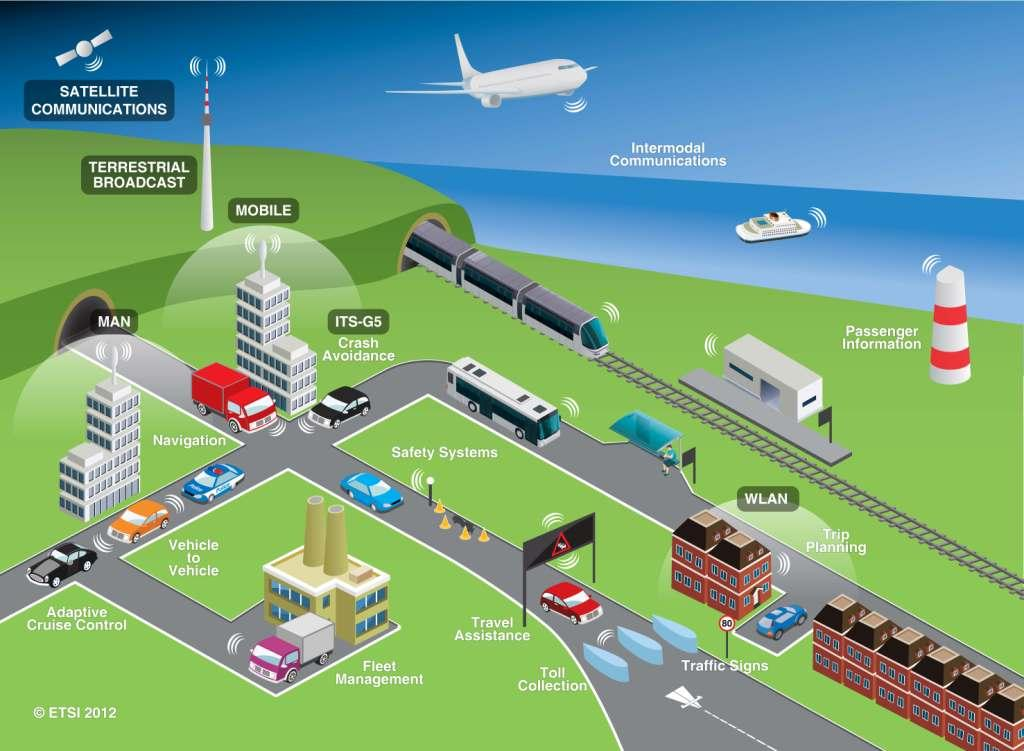
\includegraphics[width=0.95\textwidth]{content/images/00_einleitung/ETSI_ITS_09_2012.jpg}
	\caption{Übersicht über ITS \cite{ITS_vorstellung}}
	\label{fig:itsVorstellung}
\end{figure}

Die \autoref{fig:itsVorstellung} gibt einen Überblick über die Möglichkeiten von \ac{ITS} dabei ist leicht zu erkennen, dass \ac{ITS} über die reine \ac{C2C} Kommunikation hinaus geht. Das System bietet die Grundlage für verschiedene Anwendungsfälle. Sie können die verschiedensten Ziele verfolgen. So sind beispielsweise neben der Erhöhung der Sicherheit oder der Verkehrseffizienz auch Anwendungsfälle möglich, die dem Komfort der Verkehrsteilnehmer dienen. All diesen Anwendungen wird eine Plattform geboten, die die Zuverlässigkeit des Systems und die Sicherheit der Teilnehmer sicherstellt. So muss sich der Entwickler einer solchen Anwendung keine Gedanken um den Datenschutz machen, da dieser bereits durch \ac{ITS} sichergestellt wird.

Die folgende Ausarbeitung soll dem Leser das \ac{ETSI} \ac{ITS} System näher bringen und ihm einen Überblick über den Aufbau, die Funktion und die Leistungsfähigkeit vermitteln. Bei der Entstehung der Ausarbeitung sind die Forschungsgruppen und Konsortien nicht berücksichtigt worden, obwohl ein Großteil der Arbeit dort erledigt wurde und wird. Die Ausarbeitung bezieht sich lediglich auf die Standards, die vom \ac{ETSI} veröffentlich wurden. Einige der Konzepte muten abstrakt an. Sie werden erst bei der Implementierung durch die \ac{OEM} oder Forschungsgruppen konkret.

\section{Begriff Car to Car}
Der Begriff \ac{C2C} beschreibt die reine Kommunikation zwischen \ac{ITS} fähigen Fahrzeugen. Dabei wird die Luftschnittstelle und die eigens hierfür entwickelte \ac{ITS} Architektur genutzt. Da diese Architektur als Gesamtes betrachtet werden muss, wird in der Ausarbeitung das gesamte \ac{ETSI} \ac{ITS} System beschrieben.  



\section{Beteiligte Konsortien}
\todo{EVtl. noch Konsortien aufzählen}


	\chapter{Funktionsweise \label{chap_funktionsweise}}

\section{IRS}

\section{IVS}

\section{ICS}

	\chapter{Architektur  \label{chap_archtitektur}}
Die Netzwerkarchitektur von \ac{ITS-S} umfasst sowohl interne als auch externe Netzwerke. Laut Standard \cite{etsi302636-3}, bzw. Standard \cite{etsi102636-3} sind dabei folgende externe Netzwerke erfasst:

\begin{itemize}
 	\item ITS ad hoc network.
	\item Access network (ITS access network, public access network, private access network).
	\item Core network (e.g. the Internet).
\end{itemize}

Auf der Grafik \ref{fig:architektur_ueberblickNetzwerke} sind die verschiedenen Netzwerke visualisiert. Diese Art der Darstellung entspricht der höchsten Abstraktionsebene. Die verschiedenen Netzwerke sind in der Grafik als Wolken dargestellt. Neben den Netzwerken sind auch die Verbindungen visualisiert.


Zusätzlich zu den hier beschriebenen Netzwerken kann eine \ac{ITS-S} ein eigenes Netzwerk, das die Teilkomponenten der \ac{ITS-S} verbindet, betreiben. Die verschiedenen Netzwerke werden benötigt, damit alle Dienste mit ihren verschiedenen Anforderungen bedient werden können.

\begin{figure}[h]
	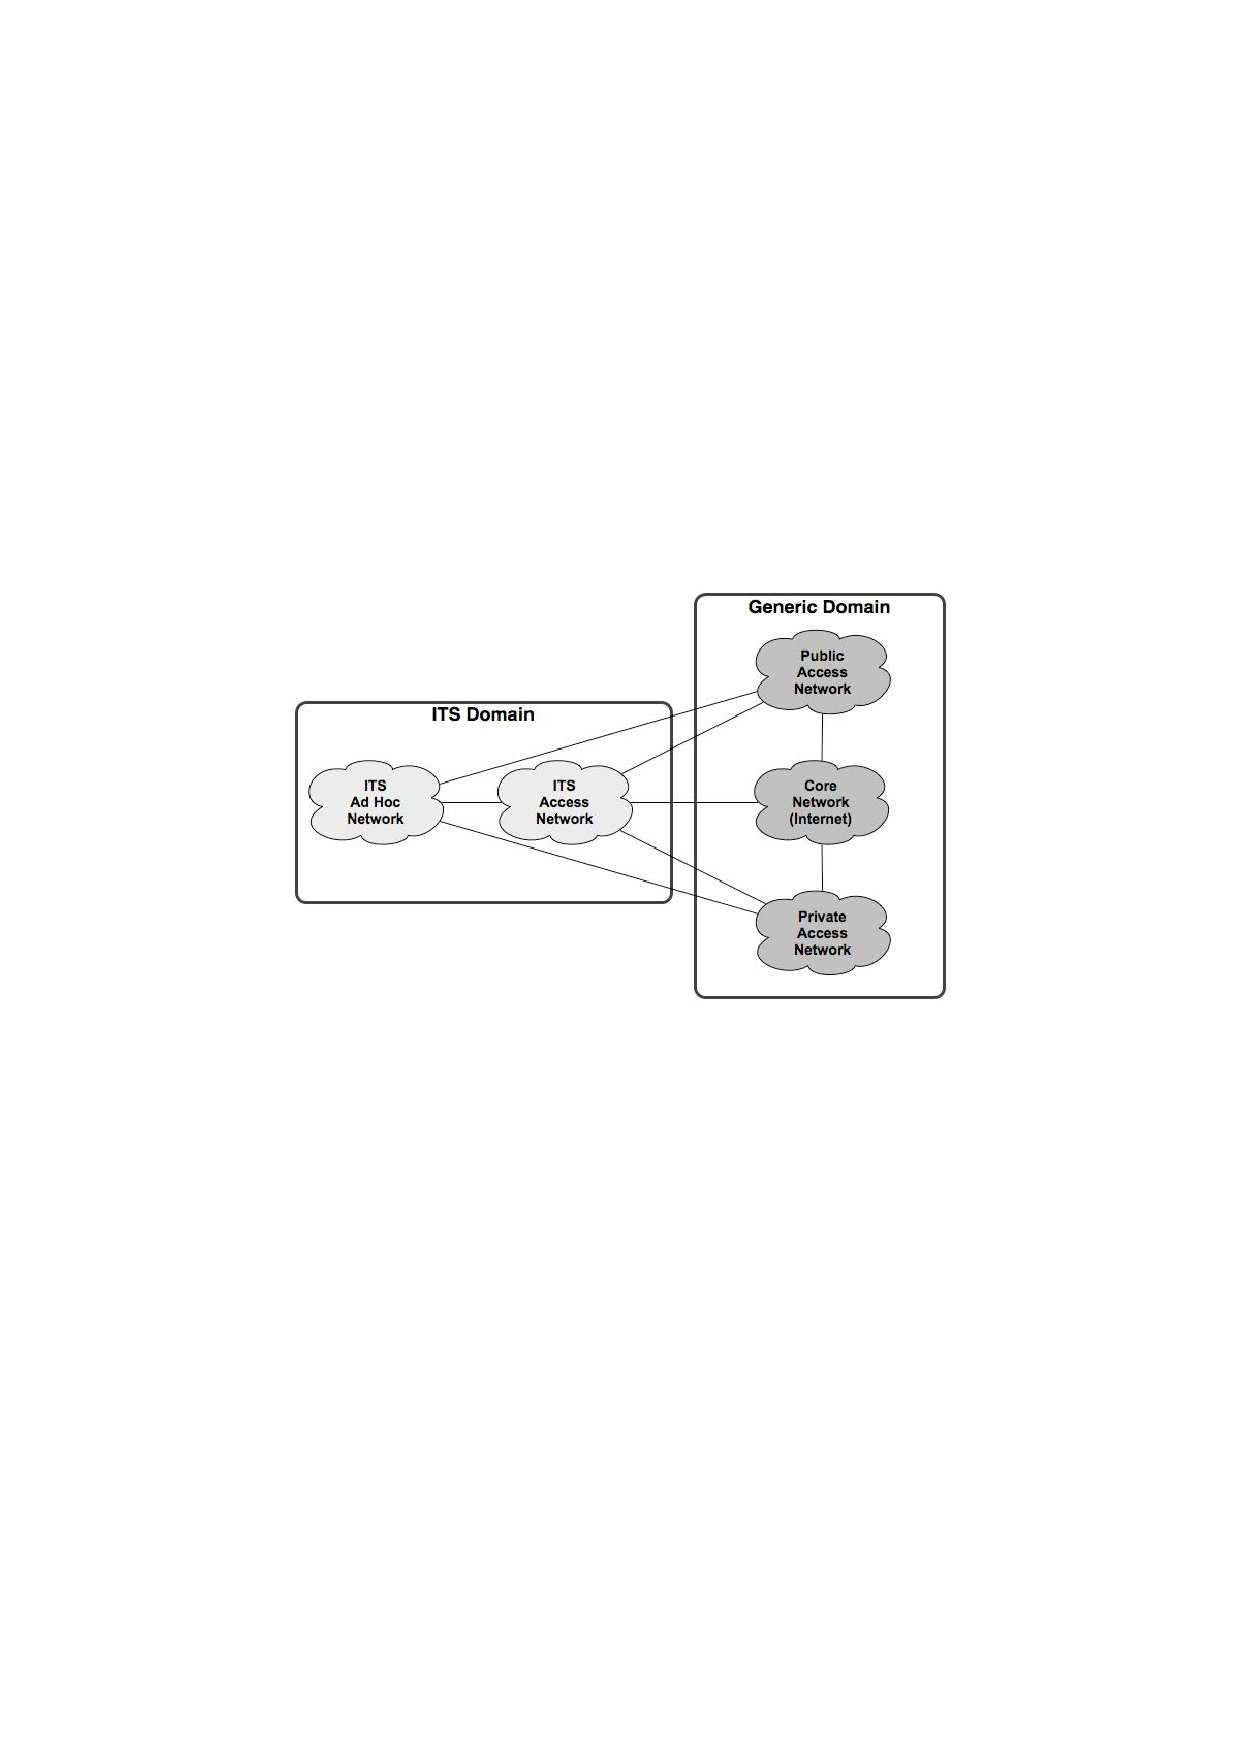
\includegraphics[width=0.99\textwidth]{content/images/02_architektur/uebersichtExterneNetzwerke.pdf}
	\caption{Überblick über die externen Netzwerke \cite{etsi302636-3}}
	\label{fig:architektur_ueberblickNetzwerke}
\end{figure}

\section{Übersicht über die verschiedenen Netzwerke \label{architektur_ueberblickNetzwerke}}
Dieser Abschnitt soll lediglich eine Übersicht über die verwendeten Netzwerke geben. Eine weitere Erklärung der Netzwerke findet an dieser Stelle nicht statt und ist nicht Gegenstand dieser Ausarbeitung. Die Netzwerke dürfen auch nicht isoliert betrachtet werden. Im Abschnitt \ref{funktionsweise_funktionaleKomponenten} wurden funktionale Komponenten mit Routingfunktionalitäten vorgestellt. Diese können die Netze und somit ihre Vorteile, bzw. ihre Dienste, miteinander verbinden.

Selbstverständlich benötigen die \ac{ITS-S} Zugang zu einem der im Folgenden aufgeführten Netze. Der Zugang zum Core Network \ref{achitektur_coreNetwork} erfolgt über eins der anderen Netze. 

\subsection{ITS Ad Hoc Network\label{achitektur_adHocNetwork}}
Das \ac{ITS} Ad Hoc Netzwerk ist das Netzwerk für die Kommunikation zwischen \ac{IRS}, \ac{IVS} und \ac{PSS}. Die Kommunikation findet über die Luftschnittstelle statt. Sie ist in ihrer Reichweite begrenzt, dafür ist sie mobil einsetzbar. Die Drahtlose Kommunikation wird im Normalfall über den Standard ITS-G5 ermöglicht.


\subsection{ITS Access Network \label{architektur_itsAccessNetwork}}
\tocheck{Nicht die blasseste Ahnung ob das mit den Access Networks stimmt}
ITS Access Network werden zur Vernetzung von \ac{ITS} Komponenten verwendet. Diese Netzwerke bieten den Zugang für die entsprechenden \ac{ITS} Services. Sie werden als eigene Netzwerke realisiert. \ac{ITS-S} werden durch Access Networks verbunden. Das bedeutet, dass \ac{IRS} untereinander über Access Networks verbunden sein können, es können aber auch Stations, die normalerweise Ad Hoc miteinander kommunizieren dieses Netz nutzen. 

\subsection{Public Access Network}
Ein Public Access Network ermöglicht den Zugang in öffentlich zugängliche Mehrzwecknetzwerke. Dieses Netzwerk kann beispielsweise dazu genutzt werden, um \ac{ITS-S} mit dem Core Netzwerk zu verbinden. 

\subsection{Private Access Network}
Ein Private Access Network reguliert den Zugang durch die Teilnehmer. Die angebotenen Datendienste stehen nur einer bestimmten Gruppe von Nutzern zur Verfügung. Mit Private Access Networks besteht die Möglichkeit, eine gesicherte Verbindung in ein anderes Netzwerk aufzubauen. So kann beispielsweise ein \ac{IVS} auf das Intranet einer Firma zugreifen. 

\subsection{Core Network \label{achitektur_coreNetwork}}
Das Core Network ist ein Verbindungsnetz. Es hat keine \ac{ITS} Funktionalitäten und wird im Standard auch nicht weiter spezifiziert. Es wird in Verbindung mit den Public Access Network dazu genutzt, traditionelle Dienste, wie Internet oder Email, anzubieten.
 
\begin{figure}
	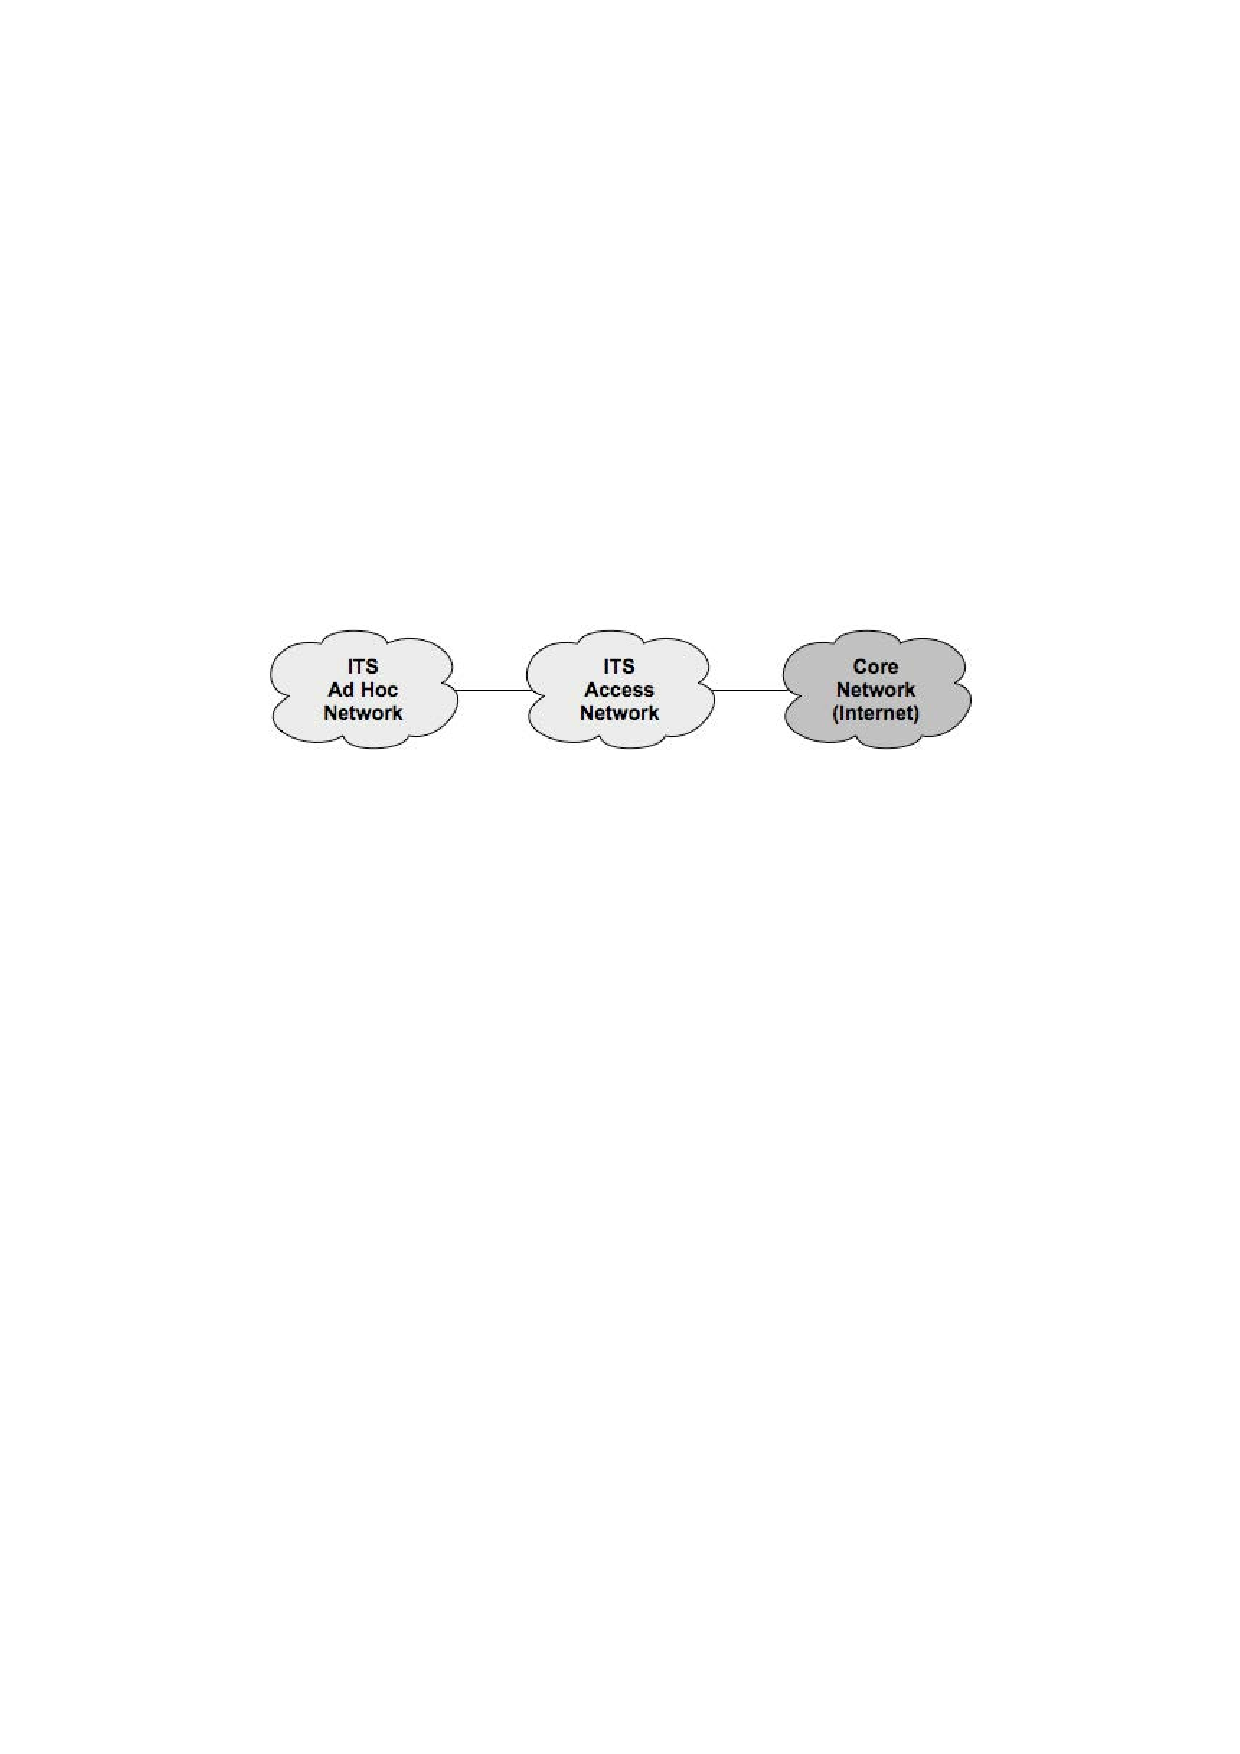
\includegraphics[width=0.75\textwidth]{content/images/02_architektur/netzwerkSzenario.pdf}
	%\vspace{2cm}
	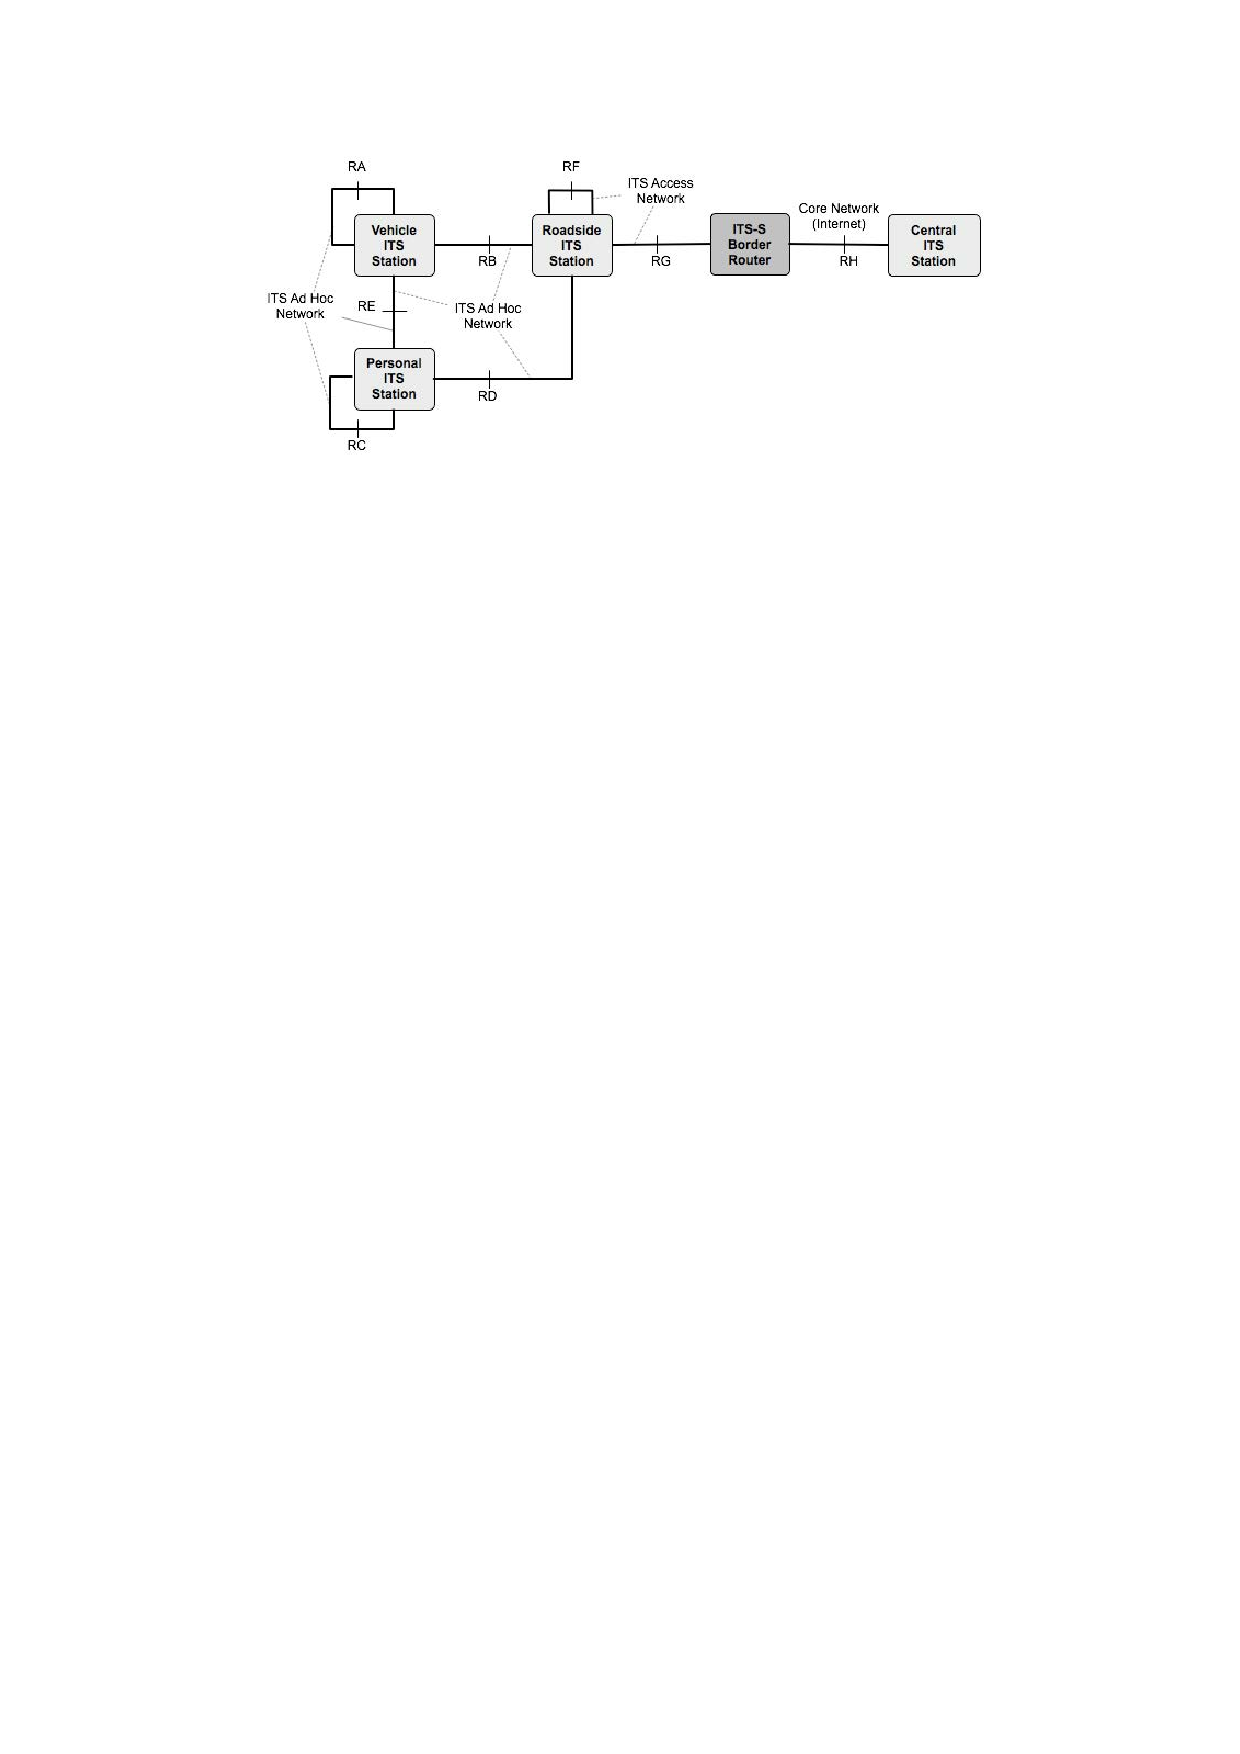
\includegraphics[width=0.75\textwidth]{content/images/02_architektur/verbindungenNetzwerkSzenario.pdf}
	\caption{Netzwerkszenario mit dazugehöriger Implementierung \cite{etsi302636-3}}
	\label{fig:architektur_netzwerkSzenario}
\end{figure}

Die Grafik \ref{fig:architektur_netzwerkSzenario} stammt aus dem Standard \cite{etsi302636-3}. Dort ist im oberen Teil der Grafik ein Szenario beschrieben, welche Netzwerke miteinander verbunden sein können.  Zu erkennen ist, dass die Netzwerke ITS Ad Hoc Netzwerk \ref{achitektur_adHocNetwork}, ITS Access Network \ref{architektur_itsAccessNetwork} und das Core Network  \ref{achitektur_coreNetwork} miteinander verbunden sein sollen.

Der untere Teil der Grafik zeigt eine Implementierungsmöglichkeit dieses Szenarios. Die hellen Rechtecke beschreiben die Komponenten, die in dieser Implementierung im System integriert sind, das dunkle Rechteck beschreibt die funktionale Komponente, die in diesem System beteiligt ist. Die Linien sind mit dem Typ des Netzwerks, welches sie repräsentieren beschriftet und zusätzlich mit dem Network Reference Point, den sie benutzen, beschriftet.
\todo{Sollen wir hier noch was zum Thema Network Reference Point schreiben? Ich glaube aber, dass die noch in den Layern kommen}


Auflistung und kurze Beschreibung der genutzten Network Reference Points:
\begin{itemize}
	\item \textbf{RA: } Reference Point zwischen \ac{IVS} über das ITS Ad Hoc Network
	\item \textbf{RB: } Reference Point zwischen \ac{IVS} und \ac{IRS} über das ITS Ad Hoc Network
	\item \textbf{RC: } Reference Point zwischen \ac{PSS} über das ITS Ad Hoc Network
	\item \textbf{RD: } Reference Point zwischen \ac{PSS} und \ac{IRS} über das ITS Ad Hoc Network
	\item \textbf{RE: } Reference Point zwischen \ac{IVS} und \ac{PSS} über das ITS Ad Hoc Network
	\item \textbf{RF: } Reference Point zwischen \ac{IRS} über das ITS Access Network
	\item \textbf{RG: } Reference Point zwischen \ac{IRS} und einem ITS-S Border Router \footnote{Der Border Router muss nicht explizit aufgeführt werden, da er als funktionale Komponente Teil einer Komponente ist. \label{ftn:borderRouter}} über das ITS Access Network 
	\item \textbf{RH: } Reference Point zwischen \ac{ICS} und ITS-S Border Router \footref{ftn:borderRouter} über das Core Network		
\end{itemize}

Erkennbar ist in dieser Implementierung, dass sich für mobile Stations Ad Hoc Netzwerke verwendet wurden. Diese haben den Vorteil, dass sie bereits in der Spezifikation mit der Luftschnittstelle ITS-G5 ausgestattet sind, was eine Mobilität erst ermöglicht. Was auch erkennbar ist, ist, dass die reinen ITS Netzwerke durch einen Border Router vom Core Network getrennt sind. Auch wenn hier nicht explizit aufgeführt, die \ac{ICS} benötigt in diesem Fall auch einen Border Router.

 
\section{ITS Station Reference Architecture}
\todo{komplette Section ITS Station Reference Architecture überarbeiten}
Eine Referenzarchitektur beschreibt ein allgemeines Modell einer Architektur. Das bedeutet, dass basierend auf dieser Architektur verschiedene Implementierungen existieren können. 

Die \ac{ITS-S} Reference Architecture unterscheidet sich grundlegend von bekannten Architekturen. Da sie während der Entwicklung an das \ac{OSI} Modell angelehnt war, ergeben sich einige Parallelen:
\begin{itemize}
	\item Trennung der einzelnen Layer
	\item Definition von Service Primitiven zwischen den Layern
	\item Die Standards beziehen die Layer auf die \ac{OSI} Layer. 
\end{itemize}

Der direkte Vergleich mit dem \ac{OSI} Modell und die Zuordnung der Layer wird in \autoref{fig:architektur_vergleichItsOsi} deutlich.

\begin{figure}[h]
	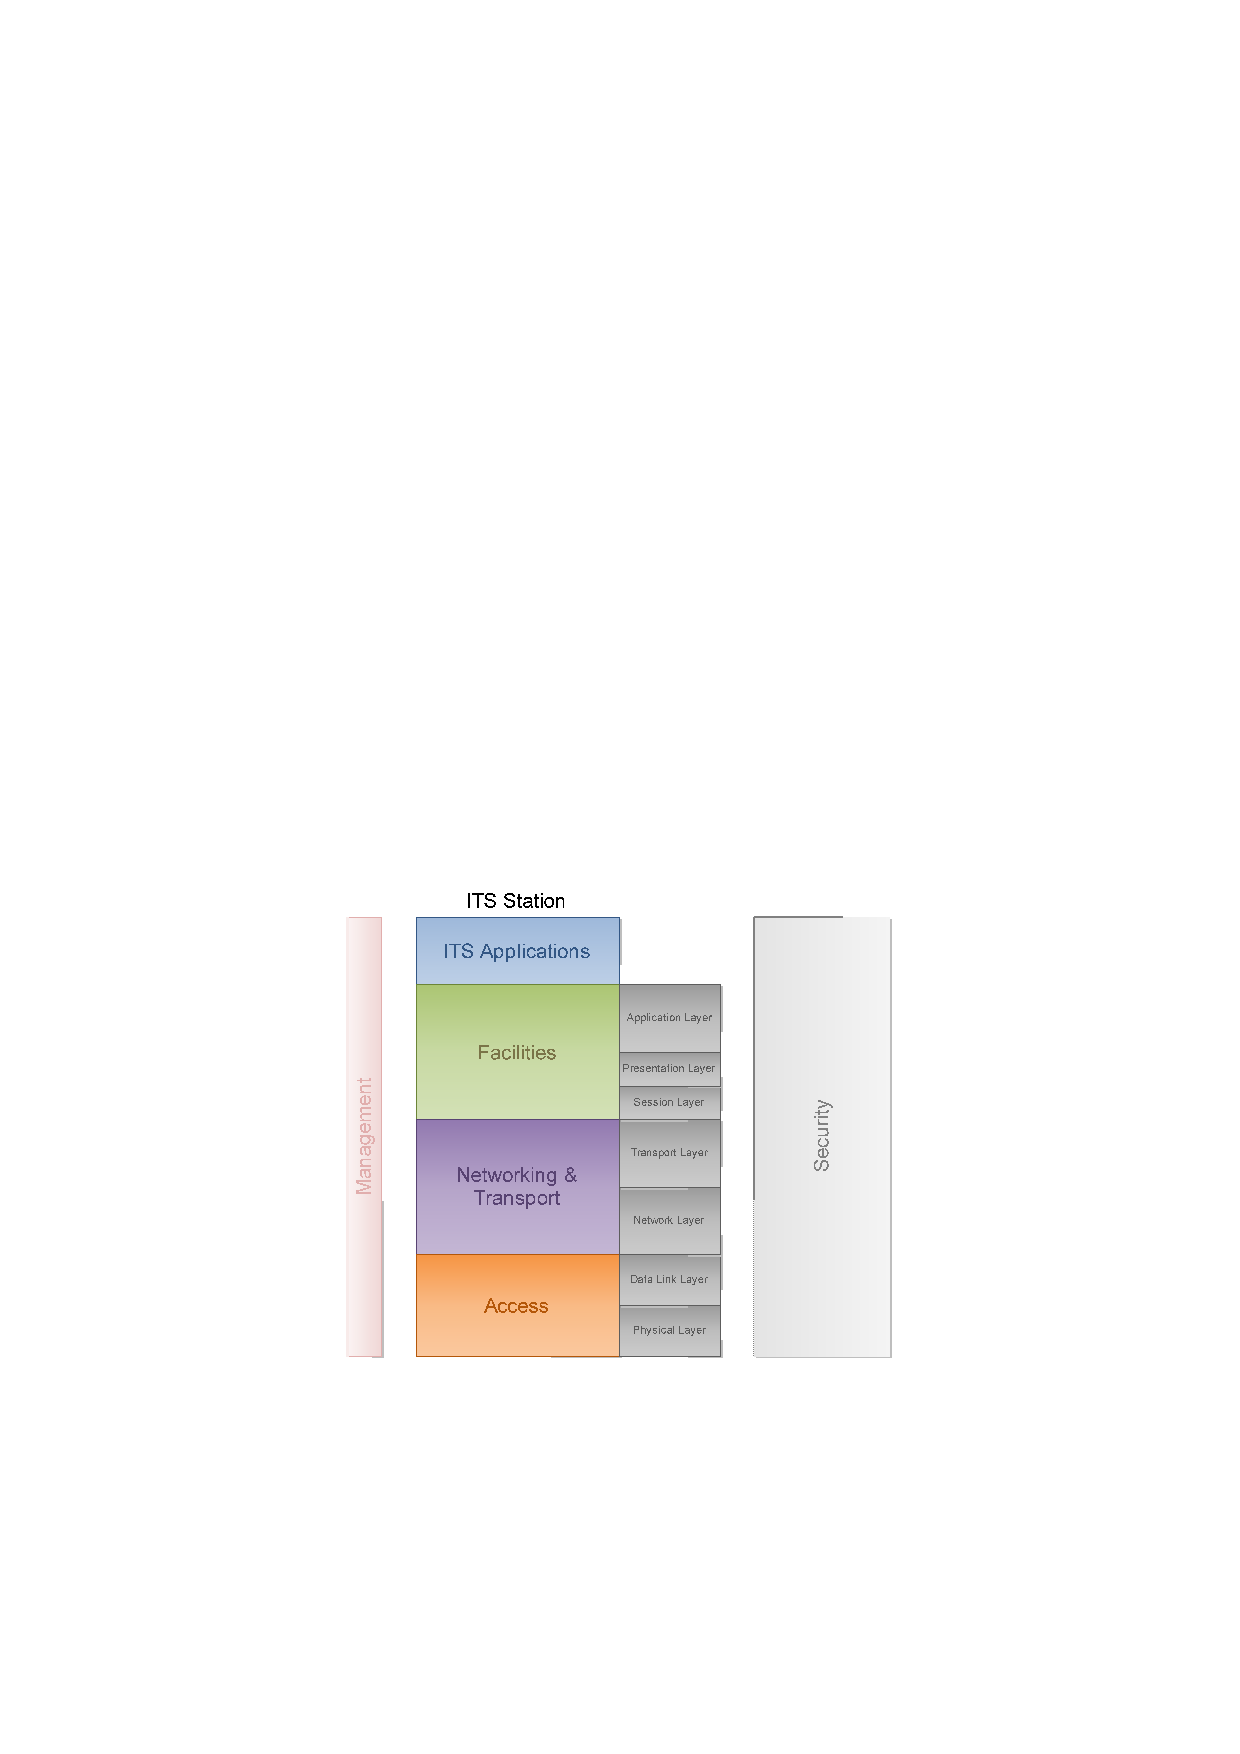
\includegraphics[width=0.99\textwidth]{content/images/02_architektur/vergleichITS-OSI.pdf}
	\caption{Der Vergleich zwischen ITS und OSI \cite{ts102940}}
	\label{fig:architektur_vergleichItsOsi}
\end{figure}

Obwohl das \ac{ITS-S} Reference Protocol bei der Entwicklung an das \ac{OSI} Modell angelehnt wurde gibt es jedoch einen gravierenden Unterschied: In der \ac{ITS-S} Reference Architecture sind Cross Layer vorgesehen. Das \ac{OSI} Referenzmodell ist wasserfallartig aufgebaut. Das bedeutet, dass die einzelnen Layer übereinander angeordnet sind. Jeder Layer hat jeweils nur zu dem direkt über- und unterliegenden Layer eine Schnittstelle. Cross Layer sind Layer, die in mehrere dieser Schichten Schnittstellen haben. Sie erweitern die vorhanden Layer in horizontaler Richtung. Im Fall der \ac{ITS-S} Reference Architecture sind das die Layer \glqq Management\grqq~ und \glqq Security\grqq. Sie haben Schnittstellen, bzw. Primitiven in alle anderen Layer. 

\begin{figure}
	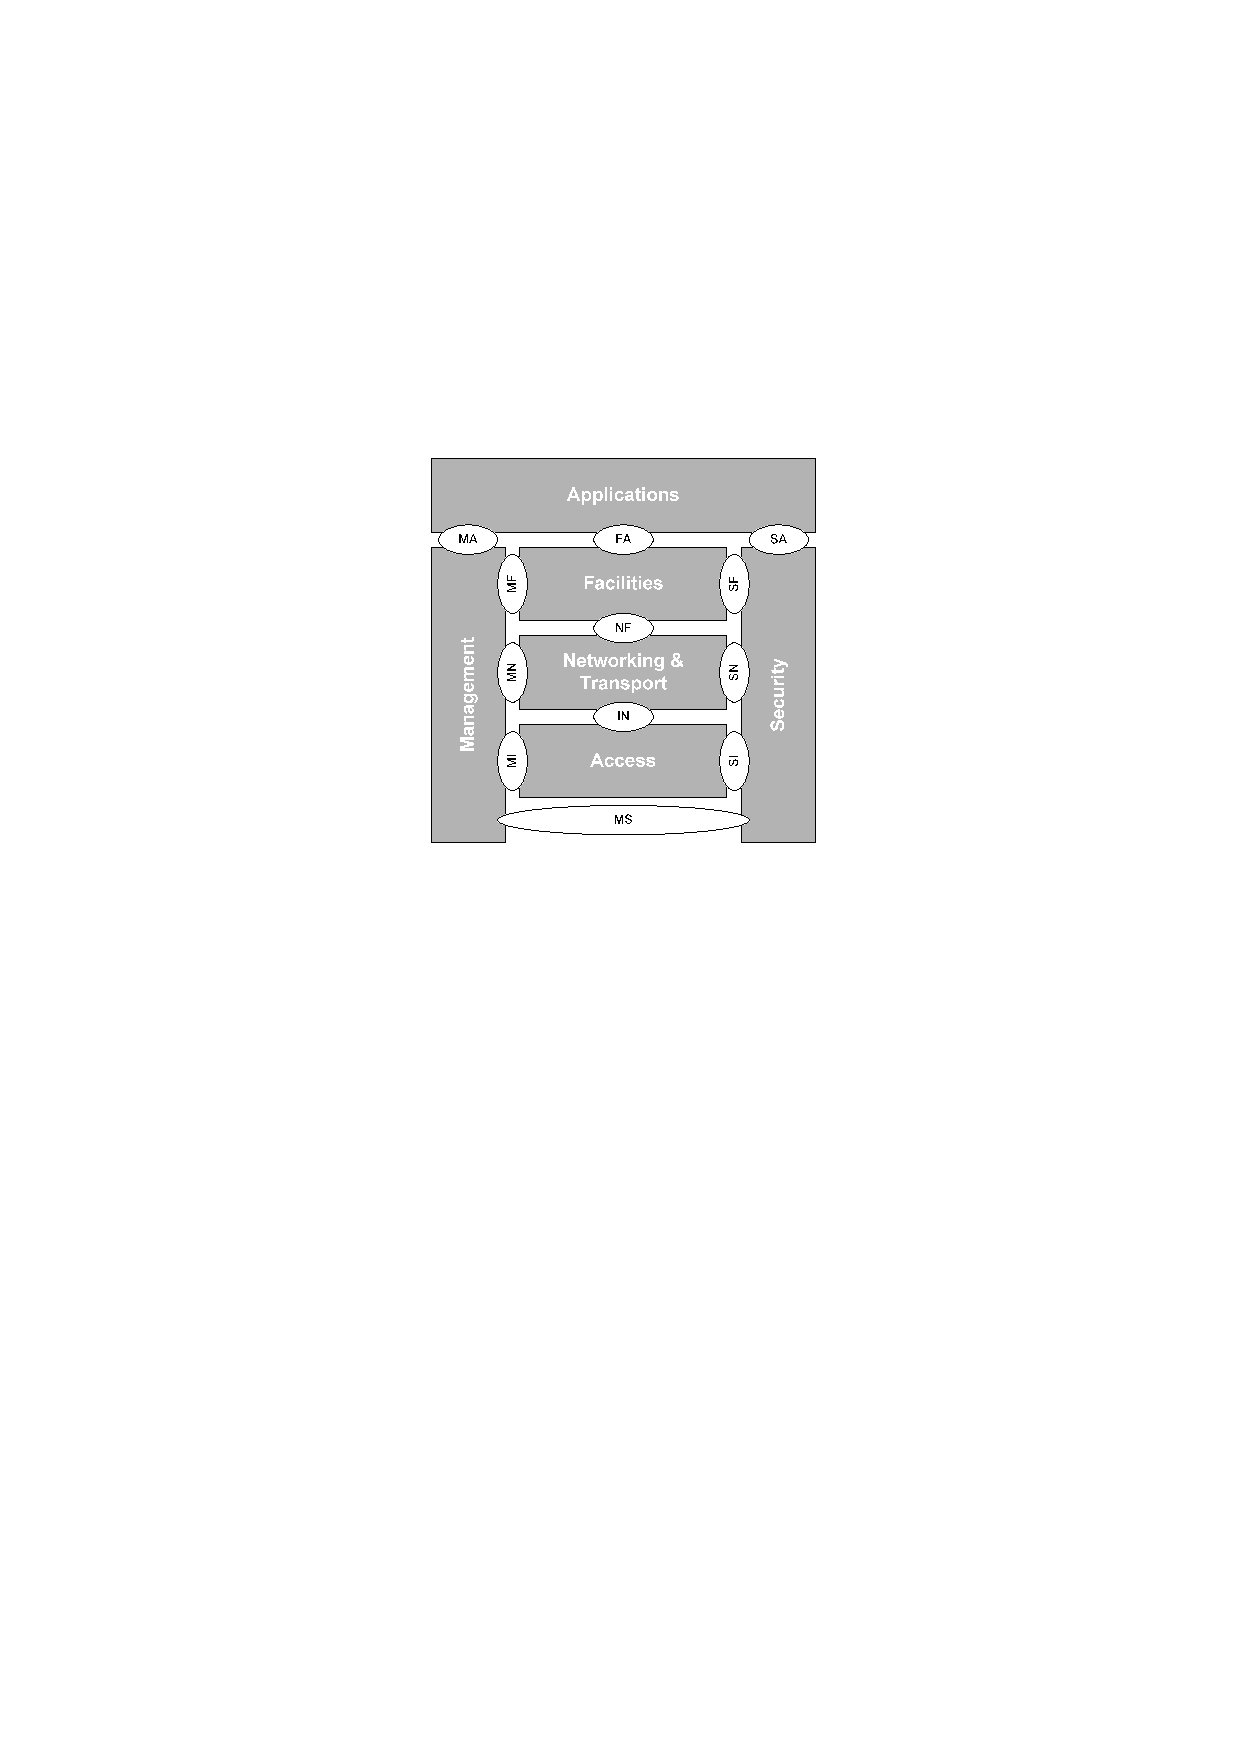
\includegraphics[width=0.75\textwidth]{content/images/02_architektur/stationReferenceArchitecture.pdf}
	\caption{Darstellung der ITS Station Reference Architecture \cite{ts102940}}
	\label{fig:funktionsweise_referenceArchitecture}
\end{figure}

\section{Horizontal Layer}
Dieser Abschnitt beschreibt die Layer, die klassisch übereinander angeordnet sind. Die Layer und ihre Funktionen entsprechen den Layern des \ac{OSI} Modells. Sie sind aber anders aufgeteilt.

\subsection{Access}
\todo{Noch etwas über die Channel herausfinden und schreiben}
Der Access Layer von ITS entspricht den \ac{OSI} Layern 1 und 2. Er besteht aus zwei Subaltern und hat drei Interfaces, bzw. \ac{SAP}. Die Sublayer sind der \glqq Data Link Layer (DLL)\grqq~und der \glqq Physical Layer (PHY)\grqq. Der DLL kann weiter in den \glqq Medium Access Control (MAC)\grqq~und den \glqq Logical Link Control (LLC)\grqq~Layer unterteilt werden. Zusätzlich zu den Subalayern hat der Access Layer ein Layer Management. Dieses verwaltet die Sublayer. Es arbeitet nur nur im Access Layer und darf nicht mit dem  Management Layer \ref{architektur_managementLayer} verwechselt werden.

Die \ac{SAP} sind:
\begin{itemize}
	\item \textbf{SAP-IN: } Als \ac{SAP} zu dem nächst höheren Layer  Networking \& Transporting \ref{architektur_networkingTransporting}
	\item \textbf{SAP-SI: } Als \ac{SAP} zu dem Cross Layer Security Layer \ref{architektur_securityLayer}
	\item \textbf{SAP-MI: } Als \ac{SAP} zu dem Cross Layer Management Layer \ref{architektur_managementLayer}
\end{itemize}
\todo{ISO 21217 finden - Scheinbar infos über die Layer}

\todo{mal in ETSI TS 102 723-10 reinsehen, ob da was interessantes zu den SAP drin steht}

Der Access Layer ist nicht auf ein bestimmtes Übertragungsprotokoll festgelegt. Beispiele für ein Übertragungsprotokoll sind ITS-G5, WiFi, BlueTooth, Ethernet\dots In einer reinen \ac{C2C} Kommunikation bietet sich aber vor allem ITS-G5 an, für eine allgemeine \ac{ITS} Verbindung haben die anderen Übertragungsprotokolle aber auch ihre Berechtigung. Diese Übertragungsprotokolle müssen aber den \ac{ITS} Protokollstack transparent übertragen. 

Der folgende Abschnitt beschreibt den Access Layer und legt G5 zugrunde.
 
\begin{figure}
	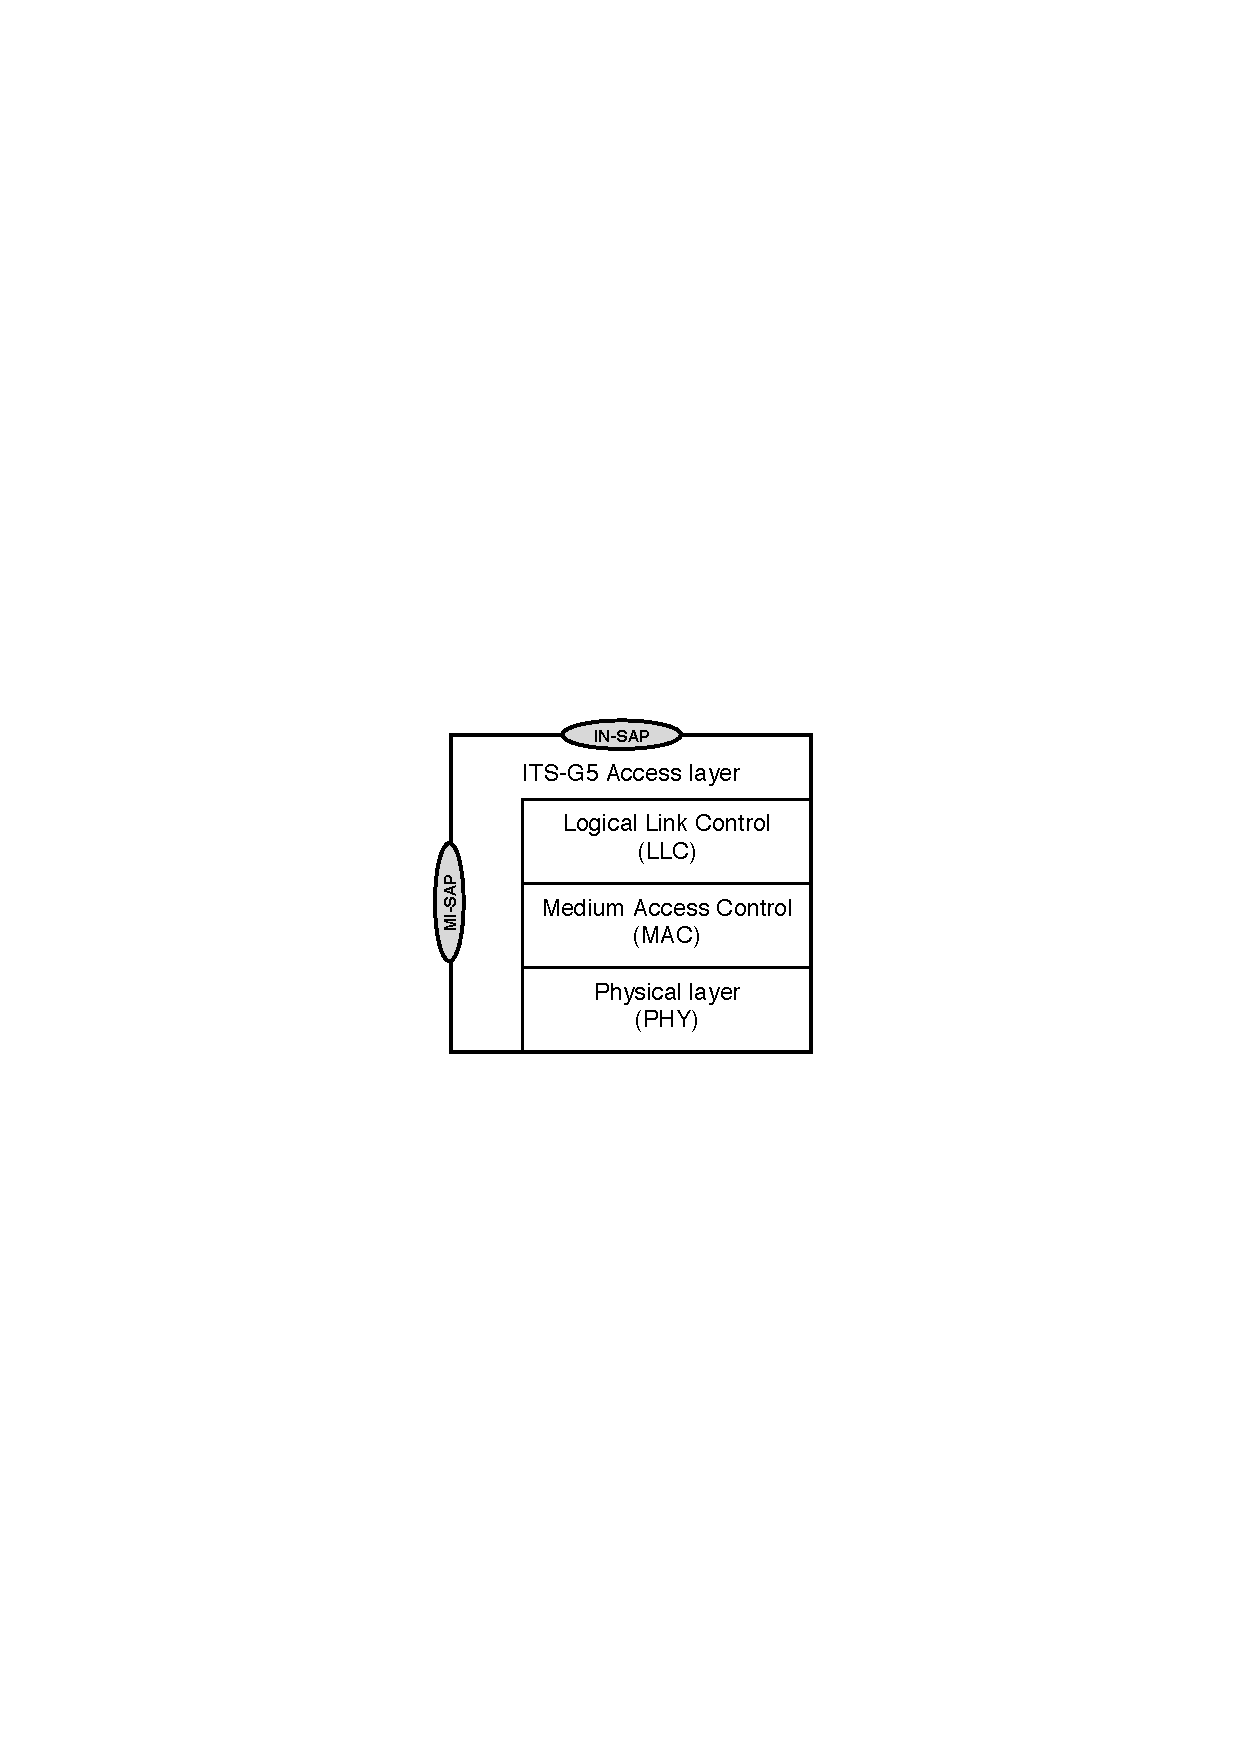
\includegraphics[width=0.75\textwidth]{content/images/02_architektur/accessLayer.pdf}
	%\missingfigure{Access Layer Bild noch aus dem Standard 302 665 herauskopieren }
	\caption{Darstellung des ITS G5 Access Layers \cite{en302665}}
	\label{fig:architektur_accessLayer}
\end{figure}

Die Grafik \ref{fig:architektur_accessLayer} entspricht des untersten Layer der Grafik \ref{fig:funktionsweise_referenceArchitecture}. In der Grafik ist zu erkennen, dass der Access Layer drei Interfaces besitzt. Er hat Interfaces zu den Cross Layern und dem Network \& Transport Layer.


Im Access Layer finden eine Periodisierung und eine Aufteilung des Datenverkehrs in Logic Channels statt. Diese Aufgaben werden mit verschiedenen Ansätzen gelöst. Deswegen sind sie keinem Sublayer genau zuzuordnen, sondern müssen in der Beschreibung der Sublayer gesondert betrachtet werden.


Eine Funktion des Access Layers ist das im Abschnitt \ref{architektur_dcc} beschriebene \ac{DCC}. Hier finden die Mechanismen Transmit Power Control (TPC), \ac{DCC} sensitivity control (DSC), Transit rate control (TRC), transmit datarate control (TDC) und DCC access control (TAC) statt. TPC regelt die Auslastung der Kanäle. Dazu werden Grenzen definiert, die TPC überwacht und einhält. TRC überwacht die Zeiten von Datenpaketen. Dazu gehören beispielsweise die Latenz eines Pakets aber auch die Intervalle zwischen Paketen. TDC überwacht die reine Datenrate eines Channels. Dabei wird nicht nur die maximale Datenrate überwacht, es wird auch beispielsweise die minimale Datenrate überwacht. DSC überwacht, ob der Sender bereit zum Senden ist. Dazu wird anhand von definierten Grenzwerten gemessen, ob der Sender am Senden ist oder nicht. TAC regelt den Kanalzugriff. \todo{Kanalzugriff erklären, wenn ich weiß, was Kanäle sind. Quelle für TAC: \cite{etsi102687}}

\subsubsection{Physical Layer (PHY)}
Der Physical Sublayer verbindet physikalisch zu dem Kommunikationsmedium.

\subsubsection{Data Link Layer (DLL)}
Der Data Link Sublayer kann wiederum in den Medium Access Control (MAC) Sublayer und den Logical Link Control (LLC) Sublayer aufgeteilt werden. Der MAC Sublayer regelt den Zugriff auf das Kommunikationmeduim.


\ac{ITS} bietet die Funktionalität von logischen Kanälen. 




\subsection{Networking \& Transporting \label{architektur_networkingTransporting}}
Der Networking \& Transporting Layer enthält mehrere verschiedene Netzwerk und Transport Protokolle und entspricht den \ac{OSI} Layern 3 und 4. Die Aufgabe ist das Routing und der Ende zu Ende Transport von Daten. Er wird im Kapitel \ref{chap:networklayer} genauer beschrieben. 


\subsection{Facilities}
Der Facilities Layer entspricht den \ac{OSI} Layern 5, 6 und 7. Er bietet eine Sammlung von Funktionen, die die \ac{ITS} Anwendungen unterstützen. Der Layer bietet Datenstrukturen um verschiedene Date zu speichern, zu sammeln und zu verwalten. Er wird im Kapitel \ref{chap:facilitylayer} genauer erklärt.

\subsection{Applications}
Im Applications Layer werden die Use Cases realisiert. Ihnen steht der \ac{ITS} Protokoll Stack zu Verfügung. Eine genauere Beschreibung des Application Layers findet im Kapitel \ref{chap:applicationlayer} statt.

\section{Cross/Vertical Layer}
Die Cross Layer weichen stark vom \ac{OSI} Modell ab. Sie erweitern die traditionellen Layer, die jeweils nur ein Interface zum nächst höheren, bzw. tieferen Layer haben um Layer, die Interfaces zu allen anderen Layern haben. Durch die Interfaces zu allen Layern ergeben sich neue Möglichkeiten. So kann beispielsweise im Application Layer die genutzte Bandbreite an die im Physical Layer zur Verfügung stehende Bandbreite angepasst werden. Dadurch werden Überlastungen, die sich auf die Latenz auswirken oder zu fehlerhaften Übertragungen führen bereits im im Vorfeld vermieden.

\subsection{Management Layer \label{architektur_managementLayer}}
Der Management Layer übernimmt Alle Aufgaben, die mit der Verwaltung einer \ac{ITS-S} und deren Protokollstack zusammenzufassen sind. Vereinfacht gesagt verwaltet er im Protokollstack die Cross Layer Funktionalität. 


\begin{figure}
	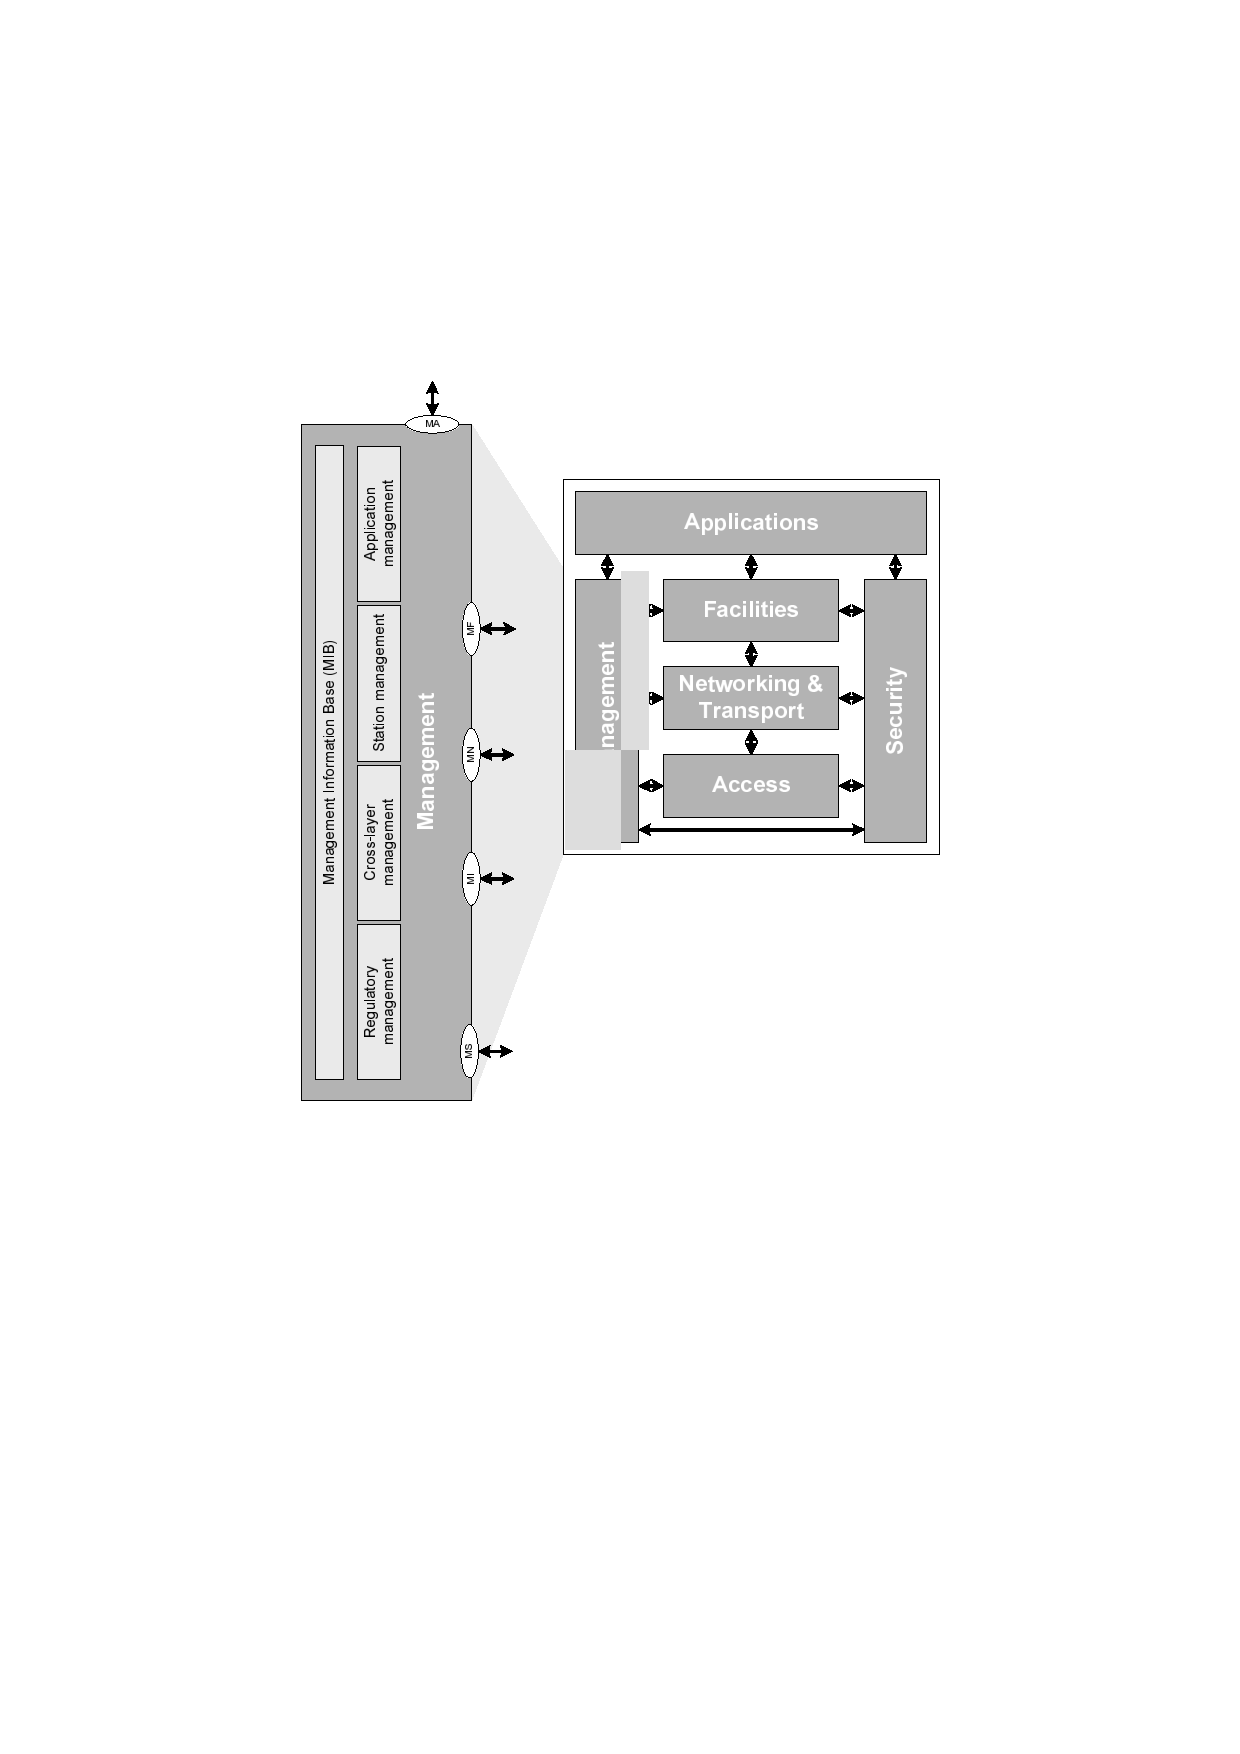
\includegraphics[width=0.75\textwidth]{content/images/02_architektur/managementLayer.pdf}
	\caption{Der Management Layer im Überblick \cite{etsi2010302}}
	\label{fig:architektur_managementLayer}
\end{figure}
\todo{Einzelne Untereinheiten der Grafik erklären, schreiben wo die beschriebenen Dienste angesiedelt sind}
In der  \autoref{fig:architektur_managementLayer} ist der Management Layer mit seinen Interfaces und Untereinheiten dargestellt. Er hat zu jedem anderen Layer ein Interface. Die fünf Untereinheiten ergeben sich aus den definierten Funktionalitäten des Management Layers. Die folgende Auflistung der Funktionalitäten ist dem Standard \cite{etsi2010302} entnommen:

\begin{itemize}
	\item Cross-interface Management
	\item Kommunikation zwischen Einheiten gem. ETSI TS 102 723-1
	\item Netzwerkmanagement
	\item Kommunikationsservice Management
	\item \ac{ITS} Anwendungs Management
	\item Station Management
	\item Management der allgemeinen Congestion Control
	\item Management des Service Advertisement
	\item Management des Systemschutzes 
	\item Eine alleine Informationsbasis
	\item Die Möglichkeit die verschiedenen Layer zu verbinden
\end{itemize}

\subsubsection{ITS Service Advertisement}
\ac{ITS} Service Adverticement ist der Mechanismus, mit dem eine \ac{ITS-S} \ac{ITS} Services erkennen kann. Bei diesem Mechanismus macht eine \ac{ITS-S}, in dem Fall der Service Provider, aktiv ihre Services anderen \ac{ITS-S}, in dem Fall Service User, bekannt. Eine Möglichkeit, die Services bekannt zu machen ist das FAST Service Advertisement. Es ist im Standard ISO/IEC 24102 definiert und eignet sich für die Luftschnittstelle mit lediglich einem Hop. Beim FAST Service Advertisement wird ein Advertisement Manager benötigt. Dieser empfängt die Service Adverticements von den anderen Service Providern und sendet die Service Adverticements der eigenen \ac{ITS-S} in regelmäßigen Abständen aus.

Für das Aussenden von Service Advertisements gibt es \ac{SAM}. \autoref{architektur_darstellungSAMHeader} zeigt den Aufbau einer \ac{SAM}. Sie besteht aus einem Header und einem Body. Der Header enthält die Elemente:

\begin{itemize}
	\item samID: Identifiziert die \ac{SAM}
	\item Version: Die Versionsnummer der \ac{SAM}
	\item stationID: Die ID des sendenden Service Providers
\end{itemize}

Der Body enthält die folgenden Elemente:
\begin{itemize}
	\item serviceList: Eine Liste mit den angebotenen Services. Sie sind nach dem Standard ISO 17419 eindeutig kodiert
	\item channelList:  Eine Information, welche Channels für die Service Operation Phase genutzt werden
	\item ipServList: Informationen über Services, die angeboten wurden und der Service Operation Phase IPv6 benötigen.
\end{itemize} 


\begin{figure}[h]
	\begin{bytefield}{40}
		\wordbox{1}{Service Advertisement Message SAM} \\
		\bitbox{16}{Header} & \bitbox{24}{Body} \\
		\bitbox{4}{samID} & \bitbox{4}{Version} & \bitbox{8}{stationID} & \bitbox{8}{serviceList} & \bitbox{8}{channelList} & \bitbox{8}{ipServList}
		\end{bytefield}
	\caption{Darstellung eines SAM Pakets}
	\label{architektur_darstellungSAMHeader}
\end{figure}

Der Service User beantwortet die \ac{SAM} mit einer \ac{CTX}. Die \ac{CTX} ist ähnlich aufgebaut wie die \ac{SAM}. In der \autoref{architektur_darstellungCTXHeader} ist eine \ac{CTX} dargestellt.

\begin{figure}[h]
	\begin{bytefield}{32}
		\wordbox{1}{Context Message CTX} \\
		\bitbox{16}{Header} & \bitbox{16}{Body} \\
		\bitbox{4}{ctxID} & \bitbox{4}{Version} & \bitbox{8}{clientID} & \bitbox{8}{servContext\-List} & \bitbox{8}{ipContext\-List}
		\end{bytefield}
	\caption{Darstellung eines CTX Pakets}
	\label{architektur_darstellungCTXHeader}
\end{figure}

Der Header der \ac{CTX} entspricht dem einer \ac{SAM}. Hier wird aber anstatt der \ac{ID} des Providers die \ac{ID} des Clients mitgesendet. Im Body unterscheiden sich die Nachrichten. 

Die Body Inhalte einer \ac{CTX}:
\begin{itemize}
	\item servContextList: Informationen über den Service Kontext, der beim Service User verfügbar ist. Kann als Antwort auf einen angebotenen Service in der serviceList der \ac{SAM} vorliegen.
	\item ipContextList: Informationen über Service Kontexte, die beim Service User verfügbar sind und IPv6 benötigen. Kann als Antwort auf einen Service, der in der ipServList der \ac{SAM} angeboten wurde vorliegen.
\end{itemize}  

Das Bekanntmachen von Services kann auf zwei Arten erfolgen. Die Möglichkeiten unterscheiden sich darin, dass bei der ersten Möglichkeit die \ac{SAM} vom Service User mit einer \ac{CTX} beantwortet wird. Bei der zweiten Möglichkeit wird die \ac{SAM} nicht beantwortet. Grundsätzlich laufen die Möglichkeiten aber gleich ab.  

Die Kommunikation zwischen User und Provider kann man in zwei Phasen aufteilen. Die Service Initialization Phase und die Service Operation Phase.

Der Zweck der Service Invitation Phase ist es die Session aufzubauen. Dabei wird der Service User mit einer \ac{SAM} eingeladen. Während der Service Invitation Phase wird zwischen den beschriebenen Möglichkeiten unterschieden. Ob eine \ac{SAM} von einer \ac{CTX} bestätigt wird, hängt davon ab, ob es sich beim Service User um eine \ac{ITS} application class oder eine \ac{ITS} application handelt. Der Unterschied zwischen \ac{ITS} Application Class und \ac{ITS} Application ist, dass von einem Application Objekt mehrere Kontexte existieren können. Jeder Kontext kann auf eine \ac{ITS} Application referenziert werden. Bei der Übertragung wird der Unterschied durch  den \ac{ASN.1} Typ \glqq DSRCapplicationEntityID\grqq~als Markierung deutlich gemacht. 

Bei der Einladung von Application Classes wird die \ac{SAM} durch eine \ac{CTX} bestätigt. Bei Applications wird keine \ac{CTX} versendet. Die Service Invitation Phase wird als erfolgreich angesehen, sobald das erste \glqq REQUW\grqq~oder \glqq REQN\grqq~versendet wird. 

Nach der erfolgreichen Service Invitation Phase folgt die Service Operation Phase. \todo{rausfinden, was in dieser Phase statt findet}
\begin{figure} 
  \centering 
   \subfigure[Ohne Bestätigung durch CTX] {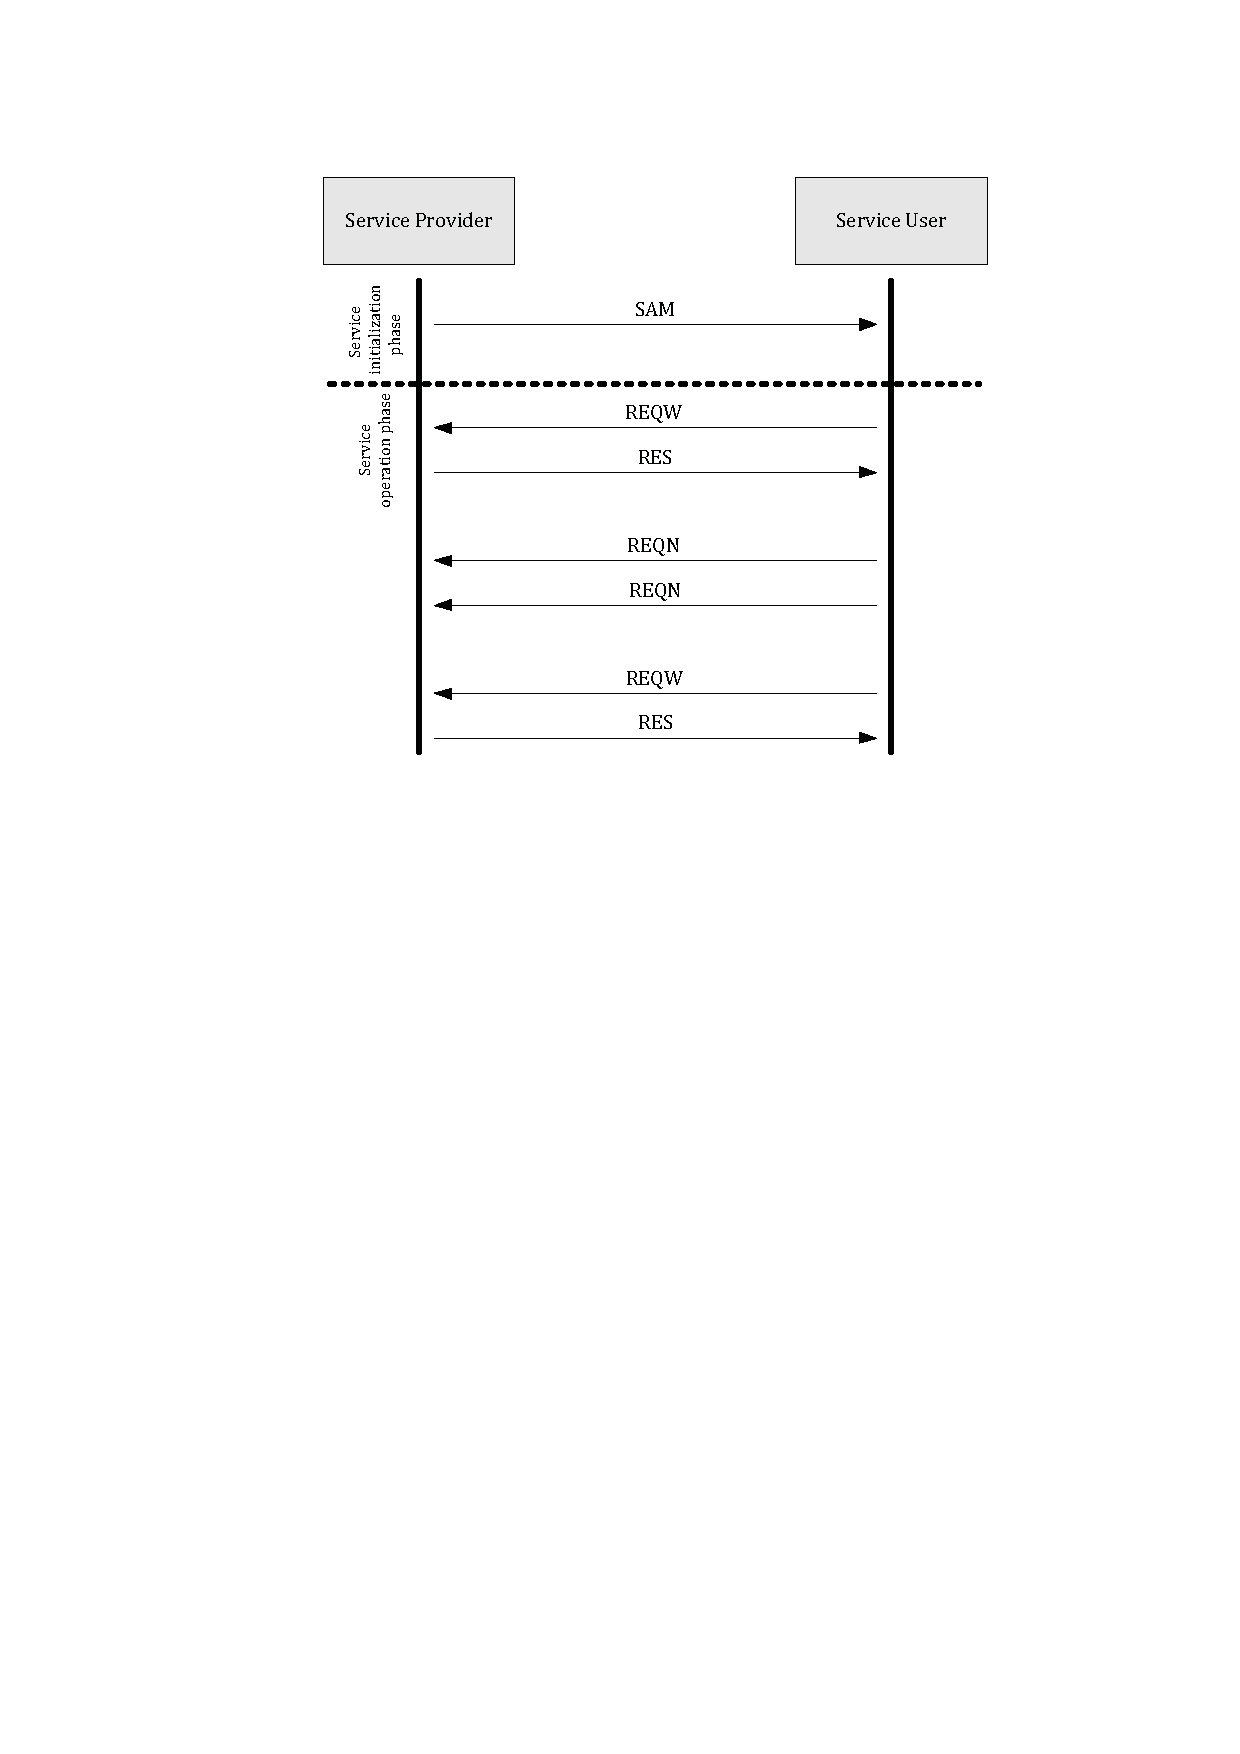
\includegraphics[width=0.45\textwidth]{content/images/02_architektur/serviceAdvertisementInit.pdf}}\qquad 
   \subfigure[Mit Bestätigung durch CTX]{ 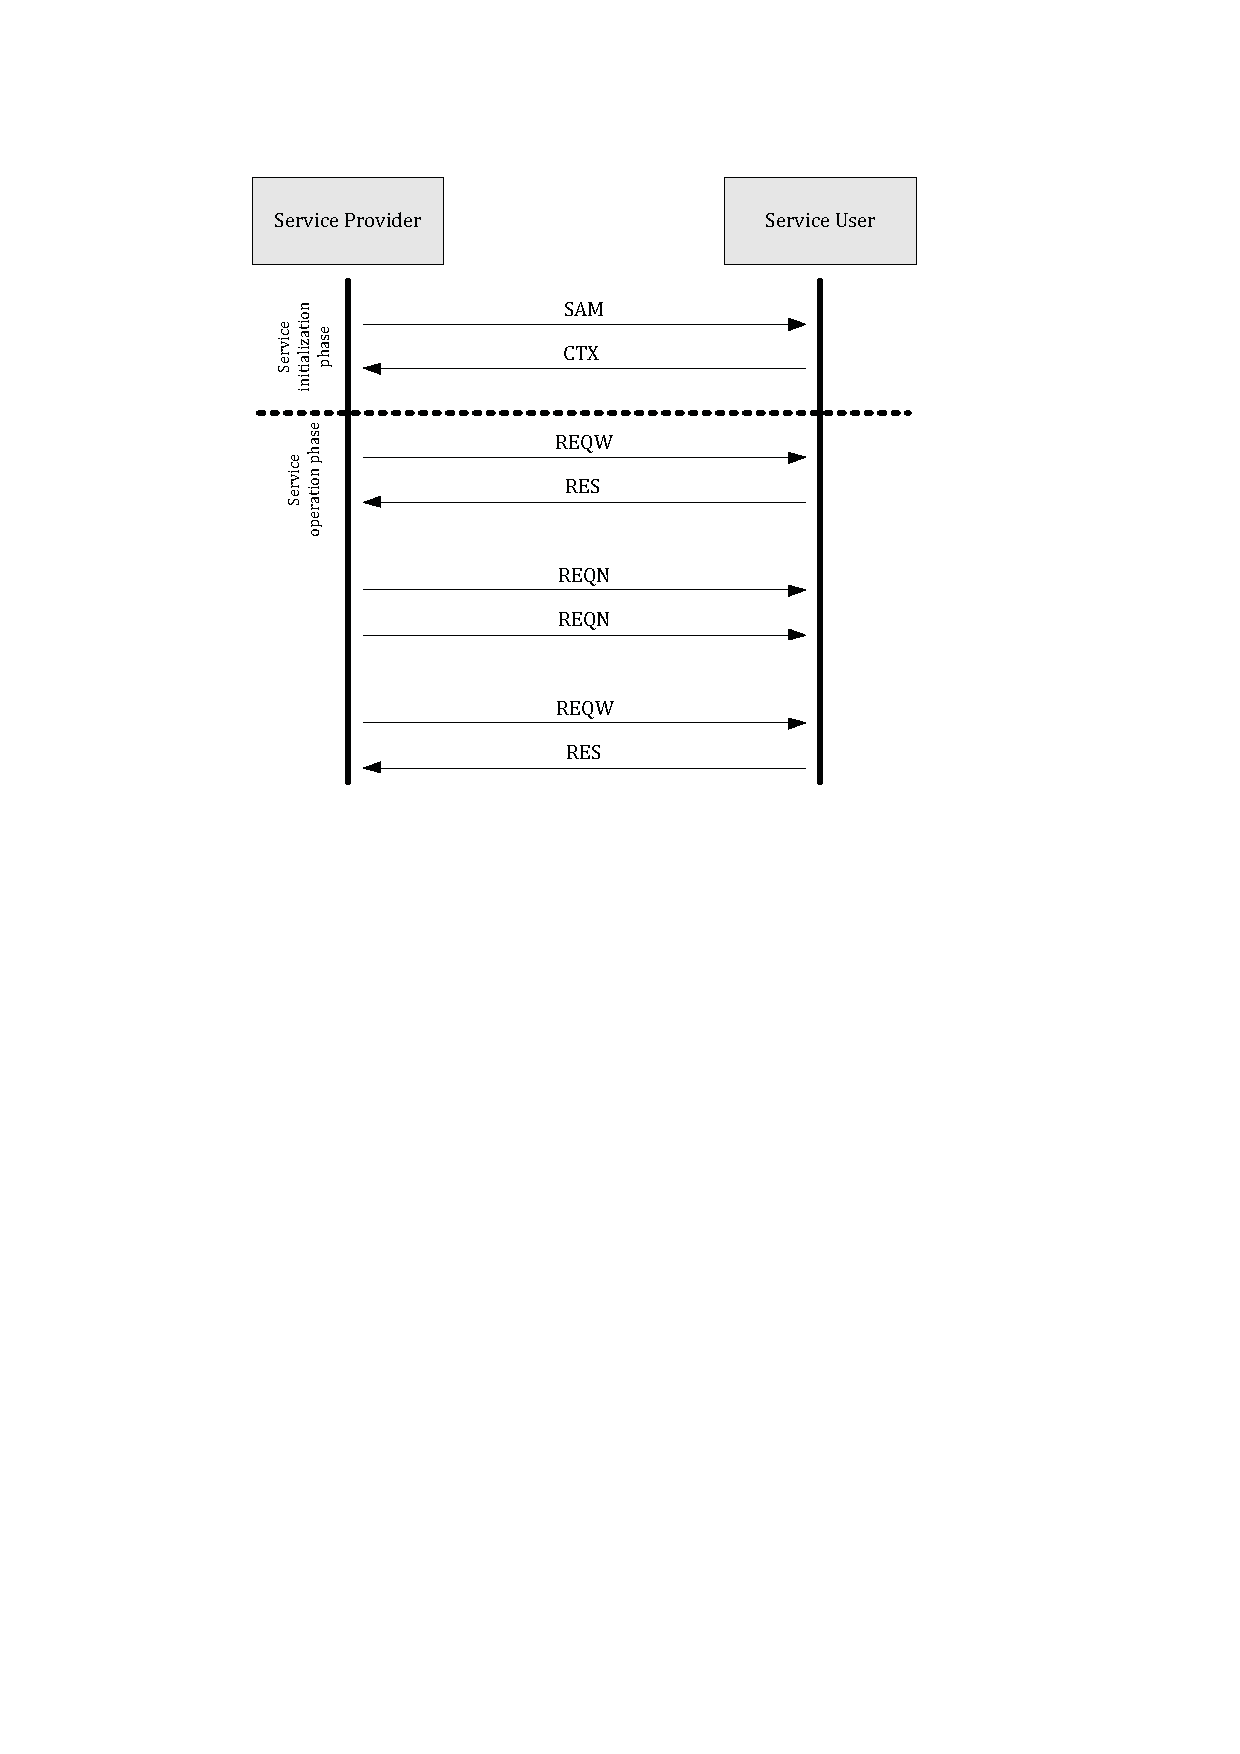
\includegraphics[width=0.45\textwidth]{content/images/02_architektur/serviceAdvertisementInitCTX.pdf}}
  \caption{Ablauf der Phasen des Fast Service Advertisement Protocol \cite{iso24102-5}} 
  \label{fig:architektur_ablaufPhasen}
\end{figure}
\todo{Prüfen, warum die Pfeile bei den Verbindungen genau umgekehrt sind}

In \autoref{fig:architektur_ablaufPhasen} wird der Ablauf der Phasen darstellt. Die einzelnen Schritte der Kommunikation bedeuten ausgeschrieben:
\begin{itemize}
	\item Request with no response expected (REQN)
	\item Request with response expected (REQW)
	\item Response to a request (RES)
\end{itemize}

Beschrieben in \cite{etsi102723-2}

\todo{Management Layer genauer beschreiben}

\todo{DCC genauer erklären und Text anpassen}

\subsubsection{Decentralizied Congestion Control\label{architektur_dcc}}
Congestion lässt sich aus dem Englischen mit Stau übersetzen. \ac{DCC} ist ein Mechanismus, der verhindern soll, dass Staus auftreten. Besonders bei \ac{ITS} Anwendungen kommt es auf zuverlässige und Übertragungswege an. Es werden hohe Anforderungen an die Verfügbarkeit und die Latenzen der Übertragungen gestellt. An Luftschnittstellen sind diese Anforderungen ohne eine Komponente wie \ac{DCC} kaum zu erfüllen. eine Der Standard \cite{etsi102687} definiert folgende Anforderungen an \ac{DCC}:
\begin{itemize}
	\item Eine faire Verteilung von Ressourcen und ein fairer Kanalzugriff zwischen allen \ac{ITS-S}en in der gleichen Kommunikationszone
	\item Die Auslastung der Kanäle muss unter vordefinierten Werten bleiben. Dies muss durch eine periodische Messung sicher gestellt werden
	\item Reservierung von Kommunikationsressourcen für das Verbreiten von hoch priorisieren ereignisgesteuerten Nachrichten
	\item Schnelle Übernahme einer wechselnden Umgebung (busy / free radio channel)
	\item Die Änderungen in den Kontrollschleifen müssen in den definierten Grenzen bleiben
	\item Es muss den spezifischen Systemanforderungen, beispielsweise Zuverlässigkeit, entsprechen
\end{itemize}

Aus diesen Anforderungen lässt sich herauslesen, dass das Vermeiden von Staus durch mehrere Mechanismen realisiert wird. Eine wichtige Eigenschaft von \ac{DCC} ist, dass es im Management Layer angesiedelt ist. Diese Tatsache ermöglicht es \ac{DCC} seine Aufgaben parallel in mehreren Layern zu realisieren. Die \ref{fig:architektur_dccArchitektur} zeigt die Architektur von \ac{DCC}. Die Abbildung zeigt den \ac{ITS} Protokoll Stack in den die \ac{DCC} Komponenten und Interfaces eingezeichnet sind. Der Vorteil dass die Layer vernetzt sind ist, dass der Stau wirklich vermieden werden kann und nicht nur die Auswirkungen des Staus behandelt werden müssen. Ein Beispiel dafür ist, dass \ac{DCC} das Trafficaufkommen bereits im Network Layer an das Medium anpassen und einzelne Dienste priorisieren kann. IEEE 802.11 beispielsweise muss bei einer Überlast, bzw. einem Pufferüberlauf, Frames verwerfen. Dieses Verwerfen muss durch Protokolle höherer Layer abgefangen werden und führt aufgrund von Retransmissions zu höheren Latenzen und einer ingesamt höheren Netzwerkauslastung. 
\todo{Stimmt das mit dem Verwerfen eigentlich?}

\begin{figure}
	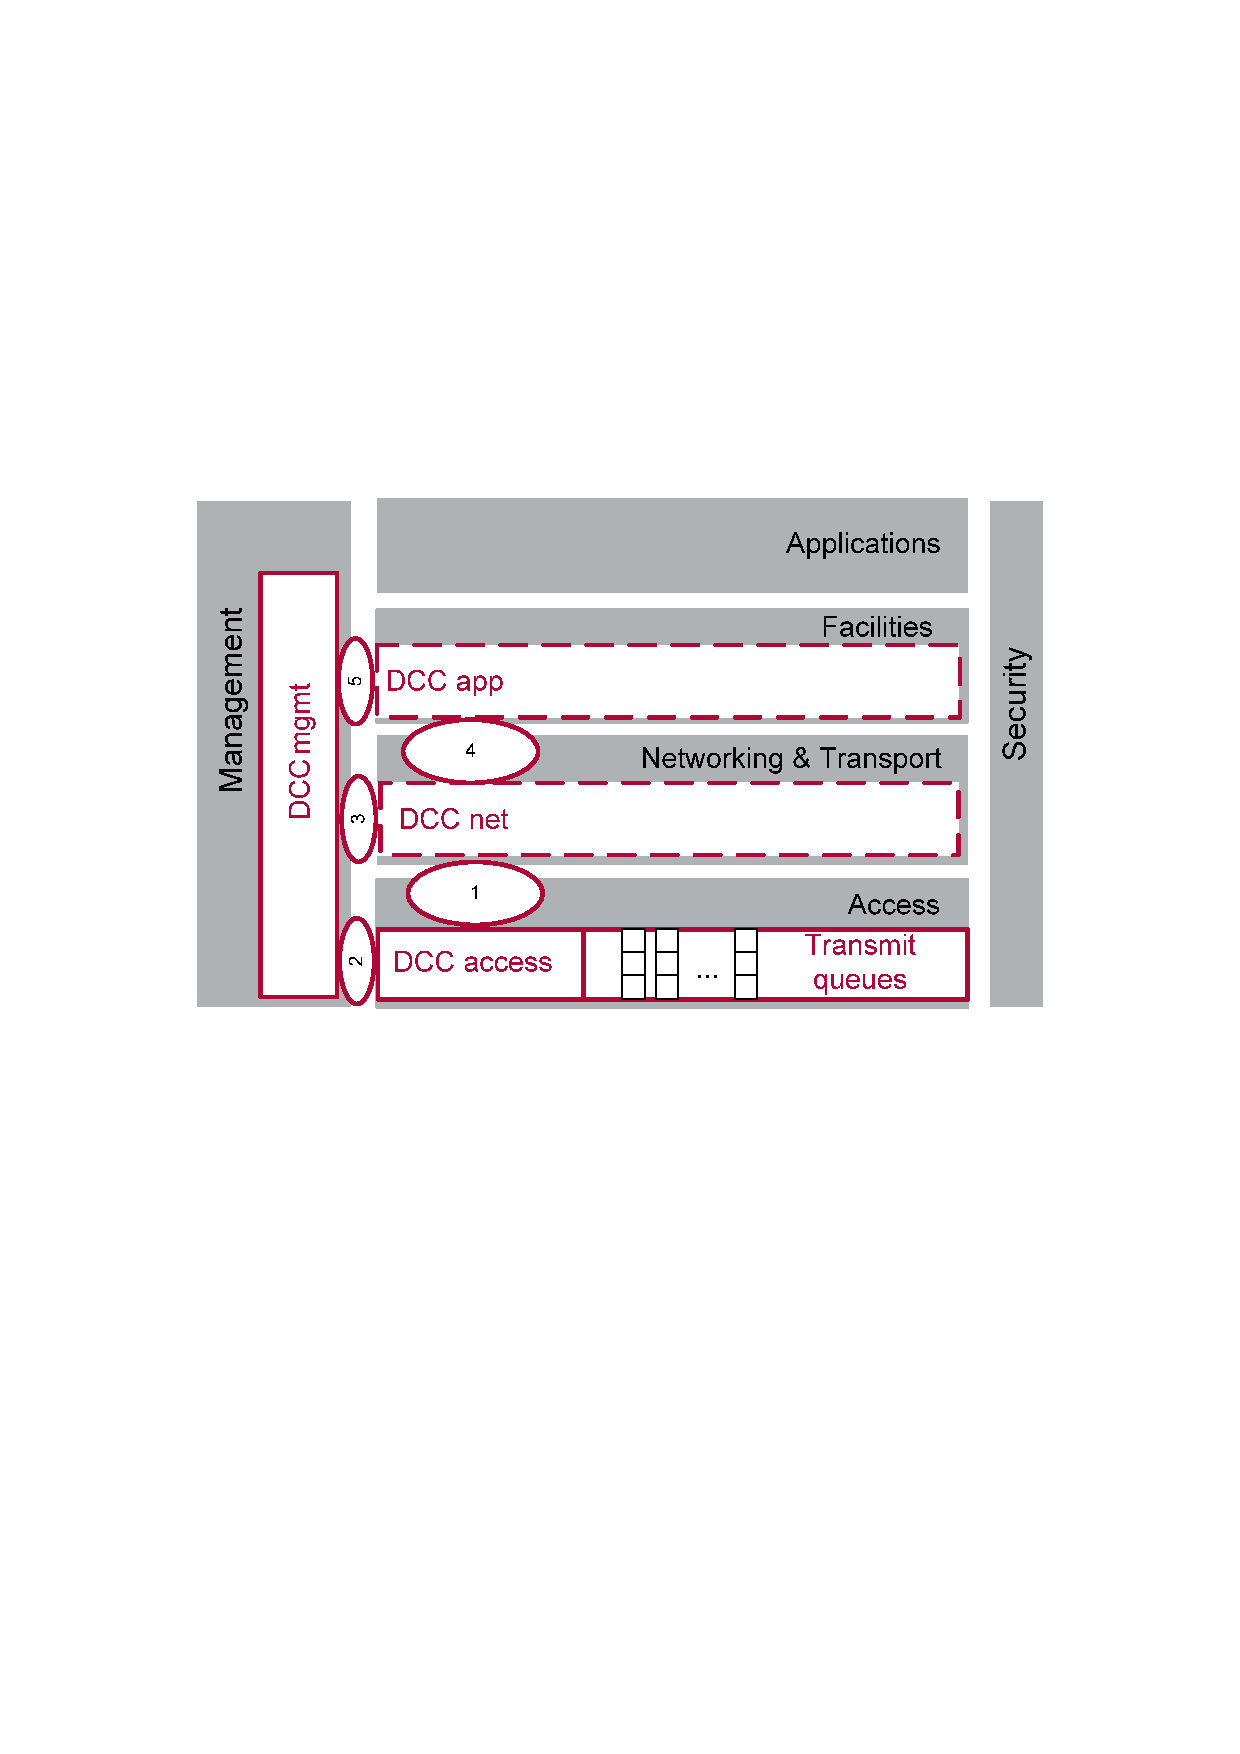
\includegraphics[width=0.75\textwidth]{content/images/02_architektur/dccArchitektur.pdf}
	\caption{Die Architektur von DCC \cite{etsi102687}}
	\label{fig:architektur_dccArchitektur}
\end{figure}

Für die Kommunikation mit mehreren Layern sind in der  \ac{DCC} Architektur vier Komponenten definiert. Die Komponenten sind mit den \ac{DCC} Interfaces verbunden, die selber auf den Interfaces der Layer zugeordnet werden. Die Komponenten werden in den Layern erklärt, in denen sie liegen. 

Die DCCmgmt Komponente ist im Management Layer angeordnet. Sie übernimmt dort die Cross Funktionalität und steuert die anderen Komponenten. Dazu hat sie Unterkomponenten.

Eine Unterkomponente der DCCmgmt Komponente ist die DCC\_CROSS\_Facilities. 



\subsubsection{CI/ITS-S application mapping}
\todo{Noch etwas über Application mapping schreiben}

\subsection{Security Layer \label{architektur_securityLayer}}
Der Security Layer ist ein Cross Layer der \ac{ITS} Architektur. Er sorgt für die Sicherheit im \ac{ITS} System. Er hat Interfaces in alle anderen Layer. 	\todo{Noch schreiben was der Security Layer genau macht} 
Der Standard \cite{en302665} beschreibt für den den Security Layer folgende Funktionalitäten:
\begin{itemize}
	\item Firewall und Angriff Management
	\item Authentifizierung, Autorisierung und Profilverwaltung
	\item Identitäts-, Krypto Schlüssel und Zertifikatsmanagement
	\item Eine allgemeine Sicherheit Informationsbasis (SIB)
	\item Hardware Security Module (HSM)
	\item Bereitstellung von Interfaces zu den anderen Layern, indem ihen Security Services angeboten werden
\end{itemize} 

\begin{figure}
	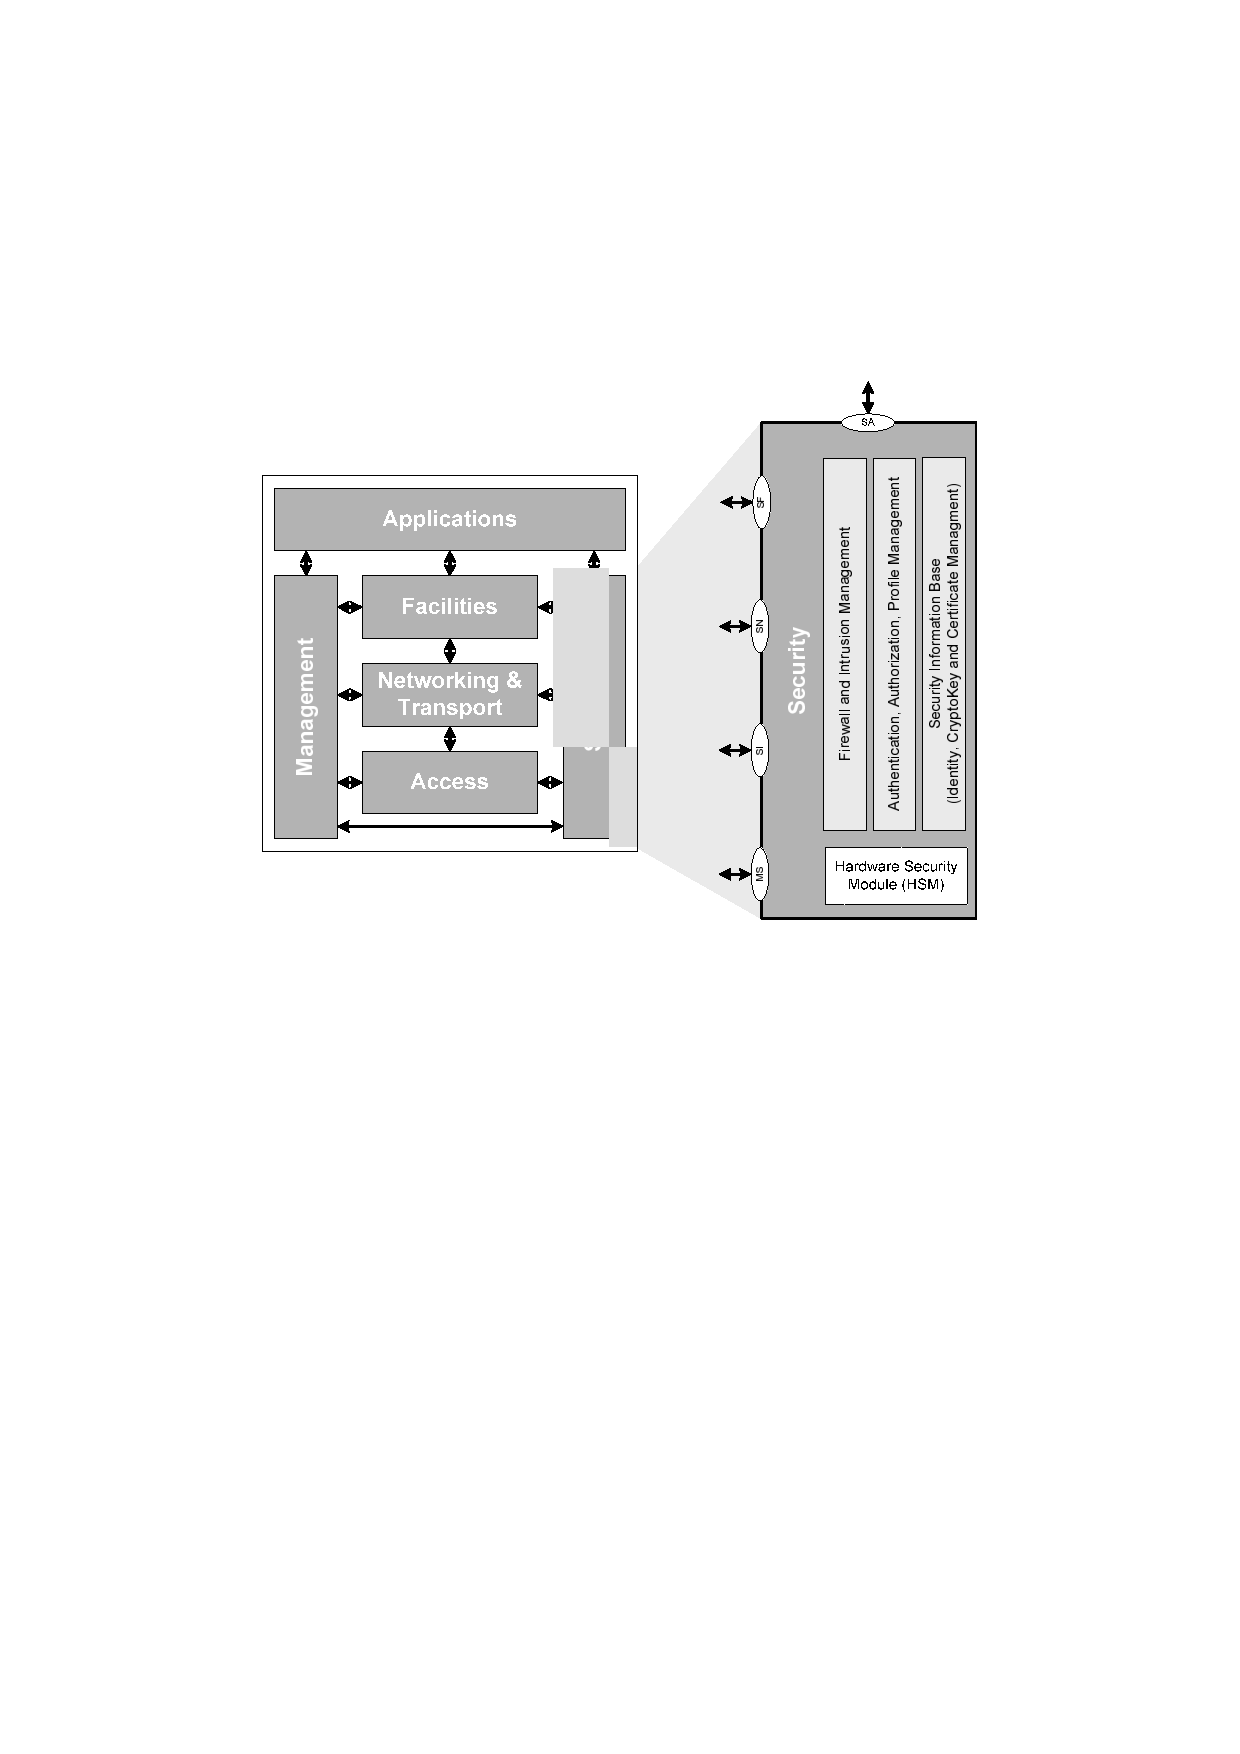
\includegraphics[width=0.75\textwidth]{content/images/02_architektur/securityLayer.pdf}
	\caption{Darstellung des Security Layers \cite{en302665}}
	\label{fig:architektur_securityLayer}
\end{figure}

\section{Data Security\label{architektur_dataSecurity}}
Der Begriff Security umfasst in \ac{ITS} verschiedene Bereiche der Sicherheit. Im \ac{ITS} Netz muss sichergestellt werden, dass die Nachrichten für die berechtigten Teilnehmer lesbar sind, für den unberechtigten Teilnehmer aber nicht. Dabei ist zu beachten, dass über \ac{ITS} sensible Daten verbreitet werden. Es muss neben dem Schutz gegen unbefugtes Lesen auch ein Mechanismus implementiert sein, der verhindert, dass falsche Informationen übertragen werden. Da die \ac{ITS} Architektur verschiedene Netzwerktypen \autoref{architektur_ueberblickNetzwerke} beinhaltet muss die Architektur auch ein Data Security Konzept beinhalten. Der Standard \cite{ts102940} spezifiziert dieses Konzept.  

\subsection{Angebotene Services}
 \begin{longtable}{| p{0.24\linewidth} | p{0.24\linewidth} | p{0.24\linewidth} |p{0.24\linewidth}|}
 \hline
 \textbf{Maßnahme} & & \textbf{Security Services} &  \\
 \cline{2-4}
 &\textbf{ First Level} & \textbf{Lower Level} & \textbf{Data Accessed}\\
 \hline
Include pseudonym in all V2V messages & Pseudonym Validation & & \\
 \hline
 Require an ITS-S to be authorized by an ITS authority before its messages are accepted by the ITS system & Obtain Enrolment Credentials & & Security Parameters (Authentication Keys)\\
 \hline
 Limit message traffic to V2I/I2V where possible & Obtain Enrolment Credentials & & Security Parameters (Authentication Keys) \\ 
 \cline{3-4}
 & & Authorization & Policy Database, Security Parameters (Authorization Ticket) \\
 \cline{3-4}
& & Establish Security Association & Security Parameters (Pseudonym, Encryption Keys) \\
 \cline{2-4}
 & Send Secured Message & Encrypt Outgoing Message & Security Parameters (Pseudonym, Encryption Key) \\
  \cline{3-4}
 &  & Authenticate Outgoing Message & Security Parameters (Pseudonym, Authentication Key) \\
 \cline{2-4}
 & Receive Secured Message & Decrypt Incoming Message & Security Parameters (Encryption Key) \\
  \cline{3-4}
 & & Validate Authentication on Incoming Message & Security Parameters (Pseudonym, Authentication Key) \\
 \cline{2-4}
 & Update Security Association & Remove Security Association & Security Parameters (Pseudonym, Encryption Key) \\
 \cline{3-4}
 & & Establish Security Association & Security Parameters (Pseudonym, Encryption Key) \\
 \cline{2-4}
 & Remove Enrolment Credentials & Authorization & Policy Database, Security Parameters (Authorization Ticket) \\
 \cline{3-4}
 & & Remove Security Association & Security Parameters (Pseudonym, Encryption Key) \\
 \hline
 Implement plausibility validation on incoming information & Validate Data Plausibility & Validate Dynamic Parameters & LDM \\
 \cline{3-4}
 & & Validate Timestamp & \\
 \cline{3-4}
 & & Validate Sequence Number &  \\
 \hline
 Include a non cryptographic checksum of the message in each message sent  & Insert Check Value & Calculate Check Value & \\
 \cline{2-4}
 & Validate Check Value & Calculate Check Value &  \\
 \hline
 Use broadcast time (Universal Coordinated Time - UTC - or GPS) to timestamp all messages & & Timestamp Message & \\
 \cline{3-4}
 & & Validate Timestamp & \\
 \hline
 Include a sequence number in each new message & & Insert Sequence Number & \\
  \cline{3-4}
 & & Validate Sequence Number & \\
 \hline
 Include an authoritative identity in each message and authenticate it & Validate pseudonym & & Security Parameters (Authentication Keys) \\
 \hline
Encrypt the transmission of personal and private data &  Send Encrypted Data & Encrypt Outgoing Message & Security Parameters (Encryption Keys) \\
\cline{2-4}
& Process Received Encrypted Data & Decrypt Incoming Message & Security Parameters (Encryption Keys) \\
\hline
Add an audit log to ITS stations to store the type and content of each message sent to and from an ITS-S &  Update Audit Log & Record Incoming ITS Messages& Audit Logs\\ \cline{3-4}
& & Record Outgoing ITS Messages & Audit Logs \\
\hline
Digitally sign each message using a Kerberos/PKI-like token & Sign Outgoing Message & Generate Signature & Security Parameters (Certificate, Keys) \\ 
\cline{3-4}
& &  Authorization & Policy database, Security Parameters (Authorization Ticket) \\
\cline{2-4}
& Verify Incoming Signed Message & Verify Signature & Security Parameters (Certificate, Keys) \\
\cline{3-4}
& & Authorization  & Policy database, Security Parameters (Certificate Status Information) \\
\hline
Use a pseudonym that cannot be linked to the true identity of either the user or the user's vehicle & Obtain Enrolment Credentials & Identification (authoritative identity provider) & Security Parameters (Pseudonym, Encryption Key) \\
\cline{2-4}
& remove Enrolment Credentials & Identification (authoritative identity provider) & Security Parameters (Pseudonym, Encryption Key)\\
\hline
Allow remote activation and deactivation of ITS-S & ITS-S Remote Management Report Misbehaving ITS-S & Authorization & Policy Database \\
\cline{3-4}
 & & Deactivate ITS Transmission & Security Parameters (Authorization Ticket) \\
 \cline{3-4}
& &  Activate ITS Transmission & Security Parameters (Authorization Ticket) \\
\cline{3-4}
& & Report Misbehaviour & Security Parameters (Authorization Ticket) \\
\hline 
\caption{Tabelle mit den Sicherheitsmaßnahmen \cite{ts102731}}
\label{tab:architektur_tabelleSicherheitsmassnahmen}
 
 \end{longtable}
\autoref{tab:architektur_tabelleSicherheitsmassnahmen} stammt aus dem Standard \cite{ts102731}. Dort werden die Maßnahmen zusammengefasst, die benötigt werden um sie zu erreichen. \glqq First Level\grqq~sind die Security Services, die direkt von den Anwendungen oder anderen Komponenten aufgerufen werden.  \glqq Lower Level\grqq~Services sind die, die von anderen Security Services aufgerufen werden.

\subsection{ITS Authoritative Hierarchy \label{architektur_itsAuthoriativeHierarchy}}
Die ITS Authoritative Hierarchy beschreibt, wer eine Rolle bei der Verwaltung der Sicherheit übernehmen kann. 

Die Hersteller von \ac{ITS-S} unterstützen die regionalen Autorisierungsstellen indem sie die Identitäten der \ac{ITS-S} verwalten. Dazu sollen sie ihnen während der Fertigung eine weltweite einzigartige Identität geben. Diese Identität soll  in Form eines Oktett Strings sein. Sie soll während der gesamten Lebensdauer gültig sein.\todo{Was will man da mit einem Oktett? Das sind 256 ITS Stations....  Original in ts 102 731: During the manufacturing process an ITS-S shall receive a globally unique canonical identity in the form of an octet string. It shall persist for the operational lifetime of the ITS-S.}
Neben der \ac{ID} müssen die \ac{ITS-S} die Fähigkeit besitzen, die Verbindung mit mindestens einer Zertifikatsstelle und mindestens einer Autorisierungsstelle zu überprüfen.  Außerdem muss sie in der Lage sein, weitere Zertifikats- und Autorisierungsstelle hinzuzufügen.

Die Zertifikatsstelle, ist eine Einheit, die die Verwaltung der Zulassungszertifikate verantwortlich ist. Die Zertifikatsstelle werden verwendet um in Nachrichten zwischen \ac{ITS-S} und einer Security Management Einheit die \ac{ITS-S} als zugangsberechtigt auszuweisen. Das beinhaltet auch die Prüfung der Identität. Die Informationen zu der \ac{ITS-S} entnimmt die Zertifikatsstelle dem Zulassungszertifikat. Sie erstellt ein neues Zertifikat, und sendet es an die \ac{ITS-S}. Dieses Zertifikat bestätigt die Identität der \ac{ITS-S} und die der Zertifikatsstelle. Es findet lediglich die Bestätigung einer gültigen Identität statt,  auf die Identität selber können mit diesem Zertifikat keine Rückschlüsse gezogen werden. Wird eine \ac{ITS-S} als kompromittiert erkannt, informiert die Zertifikatsstelle die anderen Zertifikatsstellen. Dazu wird die eideutige \ac{ID} der \ac{ITS-S} den anderen Zertifikatsstellen mitgeteilt. Die \ac{ITS-S} bekommt so lange keine neuen Zertifikate, solange sie als kompromittiert bekannt ist.  

Die Autorisierungsstelle regelt den Zugang zu allgemeinen und speziellen Diensten. Um die Dienste der Autorisierungsstelle nutzen zu können muss die die Identität der \ac{ITS-S} durch ein Zertifikat einer Zulassungsstelle nachgewiesen werden. Die \ac{ITS-S} fragt bei der Autorisierungsstelle wegen der spezifischen Berechtigungen an. Die Anfragen werden \todo{An Authorization Authority weiterschreiben} Erkennt die Autorisierungsstelle, dass eine \ac{ITS-S} kompromittiert ist, so informiert sie die Zertifikatsstelle, von der die \ac{ITS-S} ihr Zertifikat hat. Ihr werden keine weiteren Tickets mehr mitgeteilt. Zusätzlich wird werden alle anderen \ac{ITS-S} informiert, dass die Zertifikate ungültig sind.  


\subsection{Trust and Privacy Management}

Ein Aspekt der Data Security ist das Trust and Privacy Management. Der Standard \cite{ts102941} definiert für  den Begriff Privacy vier Schlüsselattribute:
\begin{itemize}
	\item Anonymity
	\item Pseudonymity
	\item Unlinkability
	\item Unobservability
\end{itemize}

Der Begriff anonymity bedeutet übersetzt Anonymität und erklärt sich von alleine. Der Begriff bedeutet, dass jemand anonymes keine Identität zugeordnet werden kann. Ein Bespiel hierfür ist eine völlig zufällige Nummer, die anstelle der Identität angegeben wird. Ihr kann keine Identität zugeordnet werden. Da einigen Services der \ac{ITS} Architektur eine Authentifizierung zu Grunde liegt ist eine vollständige Anonymisierung nicht möglich. Aus diesem Grund gibt es die drei anderen Schlüsselwörter. 

Pseudonymity bedeutet übersetzt Pseudonymisierung.  Pseudonymisierung wird oft mit Anonymisierung verwechselt, bedeutet aber etwas Anderes. Hinter etwas pseudonymisiertem steht eine Identität, die durch das  pseudonymisierte ersetzt wurde. Ein Beispiel hierfür ist die Matrikelnummer eines Studenten. Einem Angreifer, ohne die Möglichkeit, die Matrikelnummer dem Namen eines Studenten zuzuordnen, ist der Student gegenüber anonym. Besteht die Möglichkeit jedoch kann der Matrikelnummer sehr wohl eine Identität zugeordnet werden. Der Nachteil von Pseudonymen ist, dass sie wertlos sind, sobald ein Teil des Systems kompromittiert wurde. In \ac{ITS} wird die  Psyeudonymität erreicht, indem nur temporäre Kennungen von \ac{ITS-S} verwendet werden.

Ein weiterer Nachteil von Pseudonymen ist, dass mit der erfassten Datenmenge die Chance steigt, von ihnen auf eine Identität zu schließen. Wird die Nutzung eines Pseudonyms verfolgt können die Aktivitäten miteinander Verlinkt werden. Dadurch kann aus dem Pseudonym eine neue Identität werden, von der Rückschlüsse auf die Identität hinter dem Pseudonym getroffen werden können. Es kann aber auch die Identität aus dem Verhalten ermittelt werden. Um bei dem Beispiel mit dem Studenten zu bleiben, kann über ihn, bzw. seine Matrikelnummer, ein Bewegungsprofil erstellt werden, das  einzigartig ist. Wird die Matrikelnummer für das Einschreiben in Kurse genutzt kann nach genug Einschreibungen das Studienfach und das Studiensemester ermittelt werden. Diese Sammlung nennt man Verkettung von Daten. Das Schlüsselwort unlinkability fordert, dass eine \ac{ITS-S} nicht verkettbar ist. In \ac{ITS} wird die Verkettbarkeit verhindert, indem die Verwendung von nicht, oder kaum, veränderter Informationen. Damit kann Verbindungen von \ac{ITS-S} nicht anderen Verbindungen zugeordnet werden.

Unobservability bedeutet, dass der Nutzer eine Ressource nutzen kann, ohne dass andere Nutzer, oder Dritte, feststellen können, dass dieser Dienst genutzt wird.

Durch die Beachtung dieser Schlüsselwörter bei der weiteren Spezifikation und der Implementierung von \ac{ITS} wird der Datenschutz bereits im Vorfeld beachtet. 

Neben dem Datenschutz muss im \ac{ITS} System aber auch eine Zugangskontrolle realisiert werden. Die Zugangskontrolle teilt sich in zwei Bereiche auf: Die Berechtigung, das \ac{ITS} System als Ganzes zu nutzen und die Berechtigung, einzelne Services und Anwendungen zu nutzen. Die Prüfung der Identitäten wird über Zertifikate und Public-Key Verfahren realisiert. Zur Verteilung der Berechtigungen werden im Standard \cite{ts102731} definiert.

\subsection{ITS Security Serivces}
Bei den in \ac{ITS} versendeten Nachrichten müssen aus Sicht der Sicherheit drei verschiedene Typen betrachtet werden. 

Der erste Typ ist die \glqq Individual public message\grqq~Dieser Typ wird per Broadcast an andere \ac{ITS-S} versendet. Da es sich um eine Broadcast Nachricht handelt, ist eine Verschlüsselung nicht nötig. Um zu verhindern, dass mit dieser Nachricht Fehlinformationen übertragen werden muss sie lediglich signiert werden. Der Standard \cite{ts102731} nennt für diesen Typ von Nachricht die Schlagwörter: authorization, authentication und integrity. Damit wird ausgedrückt, dass die sendende \ac{ITS-S} im System legitimiert sein muss, die Nachricht wird als Schutz gegen Verfälschungen und fehlerhafte Nachrichten von Angreifern aber signiert.

Der zweite Typ ist die \glqq    Individual private message\grqq~. Sie wird an eine bestimmte \ac{ITS-S} verschickt. Da hier kein Broadcast vorliegt, macht es auch Sinn diese Nachricht zu verschlüsseln. Der Standard nennt zu diesem Nachrichtentyp die Schlüsselwörter require authorization, authentication, integrity, privacy und confidentiality. Diese Schlüsselwörter erweitern die Schlüsselwörter der \glqq Individual public message\grqq~um den Faktor, dass der Inhalt von Dritten nicht mitgelesen darf. Aus diesem Grund findet zusätzlich eine Verschlüsselung der Nachricht statt.

Als drittes sind die \glqq Security Associations\grqq zu nennen. Sie werden zwischen zwei oder mehreren \ac{ITS-S} aufgebaut und beinhalten einen Satz von Krypto Algorithmen, Schlüsseln und andere private und öffentliche Parameter. Sie werden genutzt um eine Ende zu Ende Verbindung aufzubauen.  Der Standard nennt die Schlüsselwörter confidentiality, authentication und integrity.  Diese entsprechen prinzipiell den Schlüsselwörtern der \glqq    Individual private message\grqq. Diese Verbindungen können auf andere autorisierte Teilnehmer dupliziert werden. Jeder Teilnehmer kann mehrere sichere Verbindungen haben. Wenn de sichere Verbindung aufgebaut wird, sollen die Zertifikate und die Kryptowerkzeuge die mit den sicheren Verbindungen verknüpft sind genutzt werden. Die sichere Verbindung soll ab und zu neu verhandelt werden. 

Die beschriebenen Nachrichtentypen benötigen Zertifikate. In \ac{ITS} sind zwei verschiedne Sorten von Zertifikaten definiert. Es gibt ein \glqq  authorization ticket\grqq. Es ist als ein Datenobjekt beschrieben, dass bestätigt, dass der gültige Inhaber berechtigt ist, verschiedene Aktionen auszuführen. Es wird von der ITS Autorisierungsstelle\ref{architektur_itsAuthoriativeHierarchy} ausgestellt. Die zweite Sorte Zertifikat ist das \glqq enrolment credential\grqq. Es wird als ein Datenobjekt das im Nachrichtenaustausch zwischen \ac{ITS-S} und Security Einheiten genutzt und beweist, dass der gültige Inhaber berechtigt ist, authorization tickets anzufragen. Es wird von der Zertifikatsstelle ausgestellt. Die folgenden Abschnitte erläutern wie die Verarbeitung der Zertifikate statt findet.

\subsubsection{Enrolment Credentials}
Enrolment Credentials können ausgestellt, erneuert und gelöscht werden. An diesen Tätigkeiten sind eine \ac{ITS-S} und die \ac{ITS} Infrastruktur beteiligt. Die \ac{ITS} Infrastruktur besteht in dem Fall aus einer Zertifikatsstelle und einer Autorisierungsstelle. Die \autoref{fig:architektur_enrolementFunktionalModel} beschreibt das funktionale Modell der Enrolement Credentials. Dessen Elemente werden im Standard \cite{ts102731} folgendermaßen beschrieben:

\begin{figure}[h]
	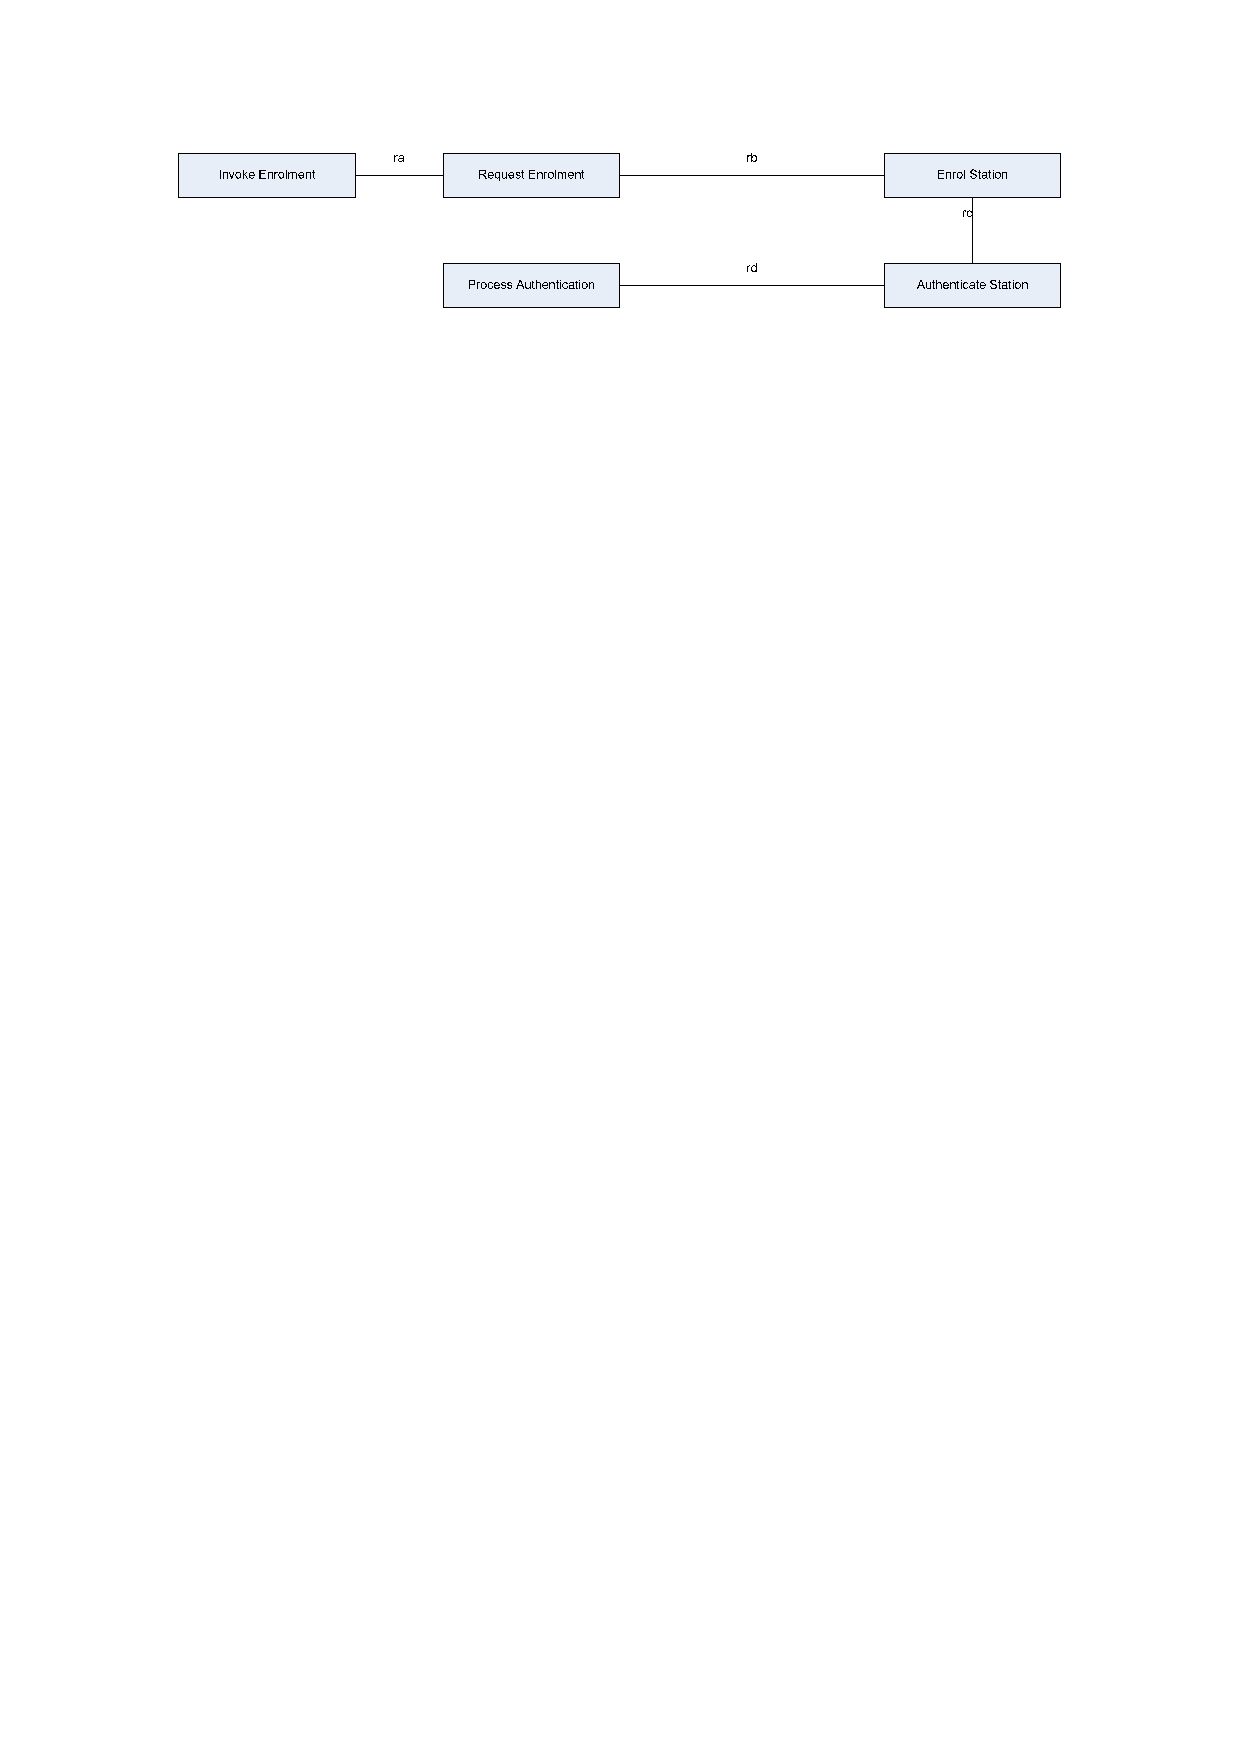
\includegraphics[width=0.75\textwidth]{content/images/02_architektur/enrolementFunktionaleKomponenten.pdf}
	\caption{Das funktionale Modell der Enrolement Credentials \cite{ts102731}}
	\label{fig:architektur_enrolementFunktionalModel}
\end{figure}

Invoke Enrolment: Dieses funktionale Element entdeckt das Bedürfnis einer \ac{ITS-S}, dass sie sich an der \ac{ITS} Infrastruktur anmelden muss und initiiert die Anmeldungsprozedur.

Enrolment Request: Dieses funktionale Element liefert die Anmeldungsanfrage für einer \ac{ITS-S} an die \ac{ITS} Infrastruktur. Anschließend empfängt es die entsprechende Antwort und speichert die geheimen Kommunikationsparameter in der \ac{ITS-S}.


Enrolement Station: Dieses funktionale Element empfängt eine Anmeldungsanfrage einer \ac{ITS-S}. Nach dieser Anfrage beginnt es den Benutzer zu authentisieren. Wenn diese Authentisieren erfolgreich war sendet es eine positive Antwort mit den Parametern, die für eine laufende sichere Kommunikation nötig sind, an die \ac{ITS-S}. Die Enrolement Station entspricht der Zertifikatsstelle. In diesem Fall ist sie als funktionales Element beschrieben. Das bedeutet, dass es in diesem Modell nur dieses eine Element gibt. 

Authenticate Station: Dieses funktionale Element validiert die Identitätsinformationen, die von dem funktionalen Element Enrol Station empfangen werden. Hierbei handelt es sich um die bereits beschriebene Autorisierungsstelle. Sie ist aber als funktionales Element beschrieben.

Process Authentication:


Das Anfordern eines enrolement credentials geschieht in zwei Schritten. Der erste Schritt ist, dass eine \ac{ITS-S} merkt, dass sie sich an der \ac{ITS} Infrastruktur anmelden muss. Dieser Schritt löst die Anmeldungsanfrage an die \ac{ITS} Infrastruktur aus.
\todo{Ausformulieren}

\todo{Evtl. noch Abschnitt über die Interfaces zu den anderen Layern 302 665 Informative Quellen}




\subsection{Access Control}

\section{Verwendete Protokolle}





	\chapter{Network Layer\label{chap:networklayer}}
Der Networklayer in der \acl{C2C}, übernimmt die Aufgabe Nachrichten durch das Netz zu Routen. Er bietet also seine Transportdienste dem Applicationlayer an. Darüber hinaus ist er für die Koordination des Netzwerkes zuständig.
Das bedeutete im genauen das er dafür Sorge trägt, dass die Nachrichten auch wirklich ankommen. Dafür beachtet er die Anforderungen der verschiedenen Anwendungen, wie z.b. das senden von Zeitkritischen Nachrichten einer Safety Application. Um bei einem Netzwerk wie es in der \acl{C2C} zu finden ist die Kommunikation zu steuern stellen sich einige Anforderungen und Herausforderungen. Vor allem bei der Adressierung der richtigen Knoten.

\subsection{Herausforderung}
Da sich die Topologie des C2C-Netzes ständig ändert, da die Knoten sich nicht nur mit unterschiedlichen Geschwindigkeiten bewegen sondern auch die Anzahl an Kommunikationspartnern sich dauernd ändert, kommt es in dem Netz zu häufigen Paketverlusten und einem allgemeinen Overhead an Informationen. Ausserdem muss gewährleistet werden das die einzelnen Fahrzeuge jederzeit wissen wie sie andere Fahrzeuge erreichen können. Zudem kommt noch hinzu das bei der hohen Informationsdichte und Komplexität des Netzwerkes noch unterschiedlich wichtige Nachrichten gesendet werden.

\subsection{Komponenten}
Im folgenden werden die einzelnen Komponenten des Networklayers genauer erläutert. Dazu wird darauf eingegangen aus welchen Komponenten der Layer besteht und wie die einzelnen Komponenten arbeiten und welche Aufgaben sie erfüllen.
\begin{figure}
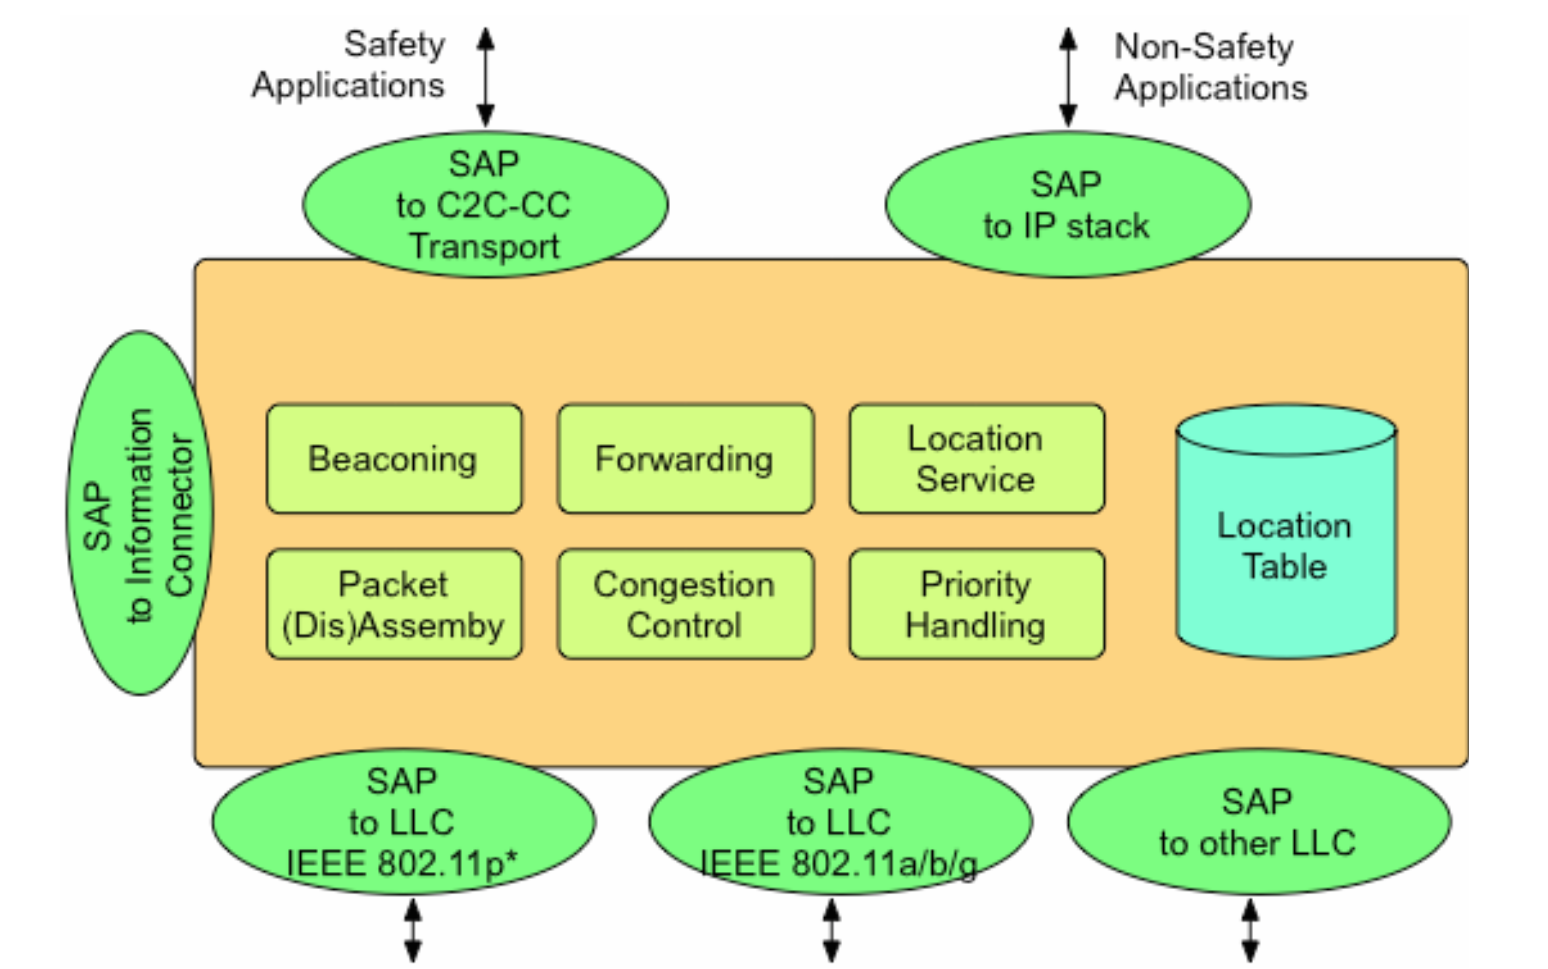
\includegraphics[width=0.99\textwidth]{content/images/03_networklayer/networklayer.png}
\caption{Die Komponenten des Networklayers\cite{C2C-manifesto}}
\label{fig:nwl}
\end{figure}
 \todo{Dateiendung von jpg zu png geändert}
Wie auf \autoref{fig:nwl} zu sehen befindet sich der Networklayer zwischen dem Aplicationlayer und dem Logical Link Control oder MAC-Layer. Das Protokoll das auf dem MAC-Layer läuft ist das, in der WLAN-Technik häufig genutzte CSMA/CA, das als bekannt vorausgesetzt wird. Es wird verwendet da sich mehrere Kommunikationseinheiten das selbe Medium teilen und es daher zu Kollisionen kommen kann. 

\subsubsection{Location Table}
\todo{neighbor tabelle hier mit einbeziehen etsi 7.1 da steht was da alles drin ist}
Jedes Fahrzeug verfügt über einen Location Table. In dieser Tabelle werden Informationen über die naheliegenden Knoten, also andere Fahrzeuge die C2C unterstützen, gespeichert. Diese Tabelle ist für das Forwarding notwendig da hier unter anderem die Adressen und Positionen der zu erreichenden Fahrzeuge gespeichert sind. 
Im Folgenden werden einige der Informationen aufgeführt die in einer solchen Tabelle enthalten sind. Jedoch können noch weitere Informationen dort gespeichert werden. Das genaue Format der Datensätze ist nicht spezifiziert und kann somit von diesem Dokument abweichen. Die Daten die in dem Location Table gespeichert sind sind nur zeitweise korrekt, daher sind sie mit einem Timestamp versehen und werden nach einer gewissen zeit verworfen. Die Informationen des Positionsvektors sollten mindestens über die unten aufgeführten Informationen verfügen. 
\begin{enumerate}
      \item C2C Netzwerkadresse
      \item MAC Adresse
      \item IPv6 Adresse
      \item Positionsvektor
      \begin{enumerate}
      	\item Geschwindigkeit
	\item Heading
	\item Geo. Position
	\item Zeitstempel des Vektors
	\item Genauigkeit des Vektors
      \end{enumerate}
      \item Version des Protokolls
      \item Typ des Fahrzeuges
      \item Zeitstempel des zuletzt erhaltenen Paketes
      \item Datenrate des ITS
      \item Direkter Nachbar Flag
\end{enumerate}

\subsubsection{Beaconing}
Um die Informationen in der Location Table zu füllen sendet jedes Fahrzeug im periodischen Abstand eine sogenannten Beacon-Nachricht an seine Umgebung. In dieser Nachricht sind die oben aufgeführten Informationen enthalten. Dadurch wird die Location Table von dem empfangenden Fahrzeug aktualisiert.

\subsubsection{Forwarding}
Der Networklayer untersützt verschiedene Arten von Forwarding Algorithmen diese werden im späteren Kapitel \autoref{sec:georouting} genauer erläutert.

\subsubsection{Location Service}
Da es durchaus vorkommen kann das der Location Table leer ist aber dennoch eine Nachricht gesendet werden muss, d.h. es wird nach einer Weiterleitungsmöglichkeit gesucht, existiert der Location Service. Über diese kann explizit nach Informationen eines Knoten gefragt werden der die Nachricht weiterleiten kann. Im vergleich zu den Beacon-Nachrichten ist der Location Service eher ein On-Demand Dienst der für Routenaufbau zuständig ist.
\begin{figure}
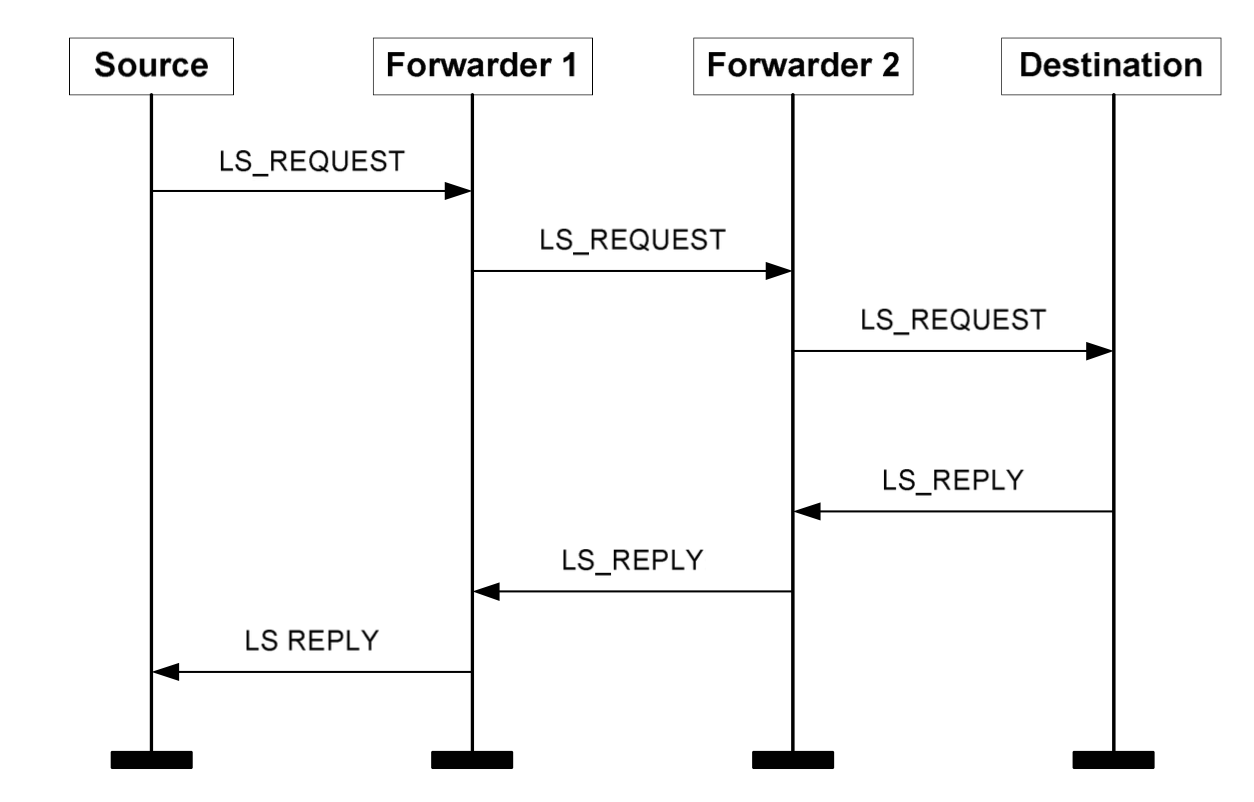
\includegraphics[width=0.99\textwidth]{content/images/03_networklayer/location-service-diagramm.jpg}
\caption{Ablauf einer Anfrage des Location Service}
\label{fig:locser}
\end{figure}
In \autoref{fig:locser} ist erkennbar wie über den Location Service Informationen des Ziels über zwei Forwarding Knoten abgerufen wird. 

\subsubsection{Priority Handling}
Anhand der Paketpriorität wird entschieden wie mit dem Paket verfahren wird. Damit wichtige Pakete zuerst gesendet werden können und andere dennoch empfangen werden gibt es eine Paketqueue in die die unwichtigeren Nachrichten eingereiht werden. 

\subsubsection{Packet Assemby}
Da sich beim versenden von Paketen die eigenen Positionsangaben sowie die Hops oder Time-to-Live ändern, muss der Networklayer dafür sorgen das die Pakete beim weitersenden modifiziert oder aktualisiert werden. Hierfür werden die Informationen aus der Location Table verwendet bevor das Paket weiter gesendet wird.

\subsubsection{Congestion Control}
Da die Paketdichte in einem C2C-Netz sehr hoch werden kann und es zu Überläufen oder Paketstaus kommen kann, muss in extremen Situationen das Netz reguliert werden. Hierauf wird in \autoref{sec:congestioncontrol} genauer eingegangen.

\section{Congestion Control\label{sec:congestioncontrol}}
\todo{Hier nochmal nachhacken ob es tatsächlich keine lösung gibt}
\todo{Ja, die gibts, nennt sich \ac{DCC} und wird im Management Layer erklärt}
Noch ungeklärt sind die Transport- und Überlastungskontrolle. Offen sind Fragen bzgl. fehlerfreiem Transport (single protocol/multiple protocols), Prioritäten von Datenpacketen, Datenaggregation und Payloadgröße. Ausfallsicherheit (connection-free/conncetion-less), Forwarding (end-to-end Prinzip), Transportarten (unicast/broadcast), Fairness, Komplexität, Multiplexing sowie Verzögerungen und Ortsgültigkeit sind auch zu klären.Es bleibt abzuwarten, wie mit den Problemen umgegangen wird. Auf Grund der vielen Anforderungen muss höchste Sorgfalt in die Entwicklung gelegt werden. Eine Herausforderung ist z.B. die Frage der Ortsgültigkeit. Unter Ortsgültigkeit ist zu verstehen, wie lange eine Nachricht in einer bestimmten Region bei der sich schnell ändernden Netzwerktopologie gültig bleibt, oder als veraltet verworfen wird.

\section{Geo Routing\label{sec:georouting}}
Um in der \acl{C2C} die richtigen Routen zu finden und die Ziele zu adressieren benötigt jeder Teilnehmer in dem Netzwerk eine einmalige Adresse. Diese ist als \acl{GNW} Adresse spezifiziert. 

\subsection{Adressierung} 
Die \acl{GNW} Adresse besteht aus acht Bytes die verschiedene Informationen repräsentieren. Die ersten zwei Bytes zeigen ob die Adresse manuell oder Automatisch konfiguriert wurde, um was es sich für ein Fahrzeug handelt und den ITS-S Country Code. Die restlichen sechs Bytes repräsentieren die MAC Adresse.\cite{etsi302636-4-1}
\begin{figure}
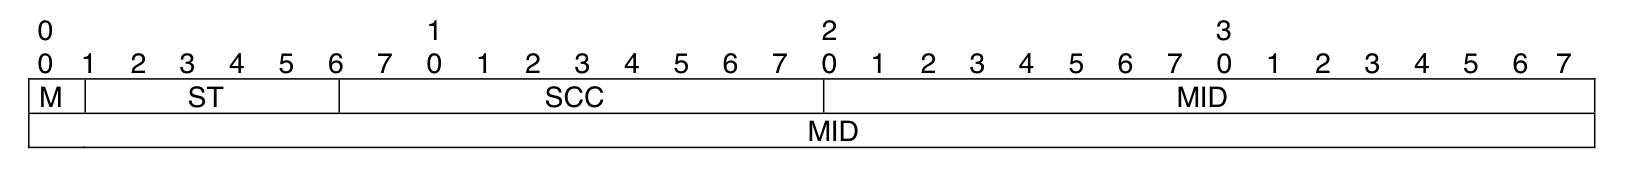
\includegraphics[width=0.99\textwidth]{content/images/03_networklayer/gnwadress.jpg}
\caption{Format der \acl{GNW} Adresse}
\label{fig:formatgnwa}
\end{figure}
Die auf der \autoref{fig:formatgnwa} zu sehenden Felder sind in der nachfolgenden \autoref{tab:formatgnwa}noch einmal genauer erläutert.

\begin{table}[h]
\begin{tabular}{lll}
Feld & Feldname & Bedeutung \\
    1 & M       & wird auf 1 gesetzt wenn die Adresse manuell vergeben worden ist, andernfalls auf 0          \\
    2 & ST    & Identifiziert um was es sich für eine ITS handelt       \\
    3 & SCC   &   ITS-S Country Code        \\
    4 & MID    &    erster Teil der MAC-Adresse       \\
    5 & MID     &   zweiter Teil der MAC-Adresse        \\
\end{tabular}
\caption{Felder und Bedeutung der \acs{GNW} Adresse\cite{etsi302636-4-1}}
\label{tab:formatgnwa}
\end{table}

Für das zweite Feld ST sind folgende Werte in \autoref{tab:typenspezi} spezifiziert.

\begin{table}[h]
\begin{tabular}{lll}
Nummer & Bedeutung  \\
    0 & Unknown \\
    1 & Pedestrian \\
    2 & Cyclist \\
    3 & Moped \\
    4 & Motorcycle \\
    5 & Passenger Car \\
    6 & Bus \\
    7 & Light Truck \\
    8 & Heavy Truck \\
    9 & Trailer \\
    10 & Special Vehicle \\
    11 & Tram \\
    15 & Road Side Unit \\
\end{tabular}
\caption{Werte für Feld zwei der \acs{GNW} Adresse\cite{etsi302636-4-1}}
\label{tab:typenspezi}
\end{table}


 \begin{itemize}
      	\item Geschwindigkeit
	\item Heading
	\item Geo. Position
	\item Zeitstempel des Vektors
	\item Genauigkeit des Vektors
\end{itemize}

\subsubsection{Konfiguration der Adressen}
\todo{siehe etsi Kapitel 9.2.1 duplicate address detection ist auch interessant}
Um eine \acl{GNW} Adresse zu konfigurieren gibt es drei Vorgehensweisen. 

\begin{enumerate}
      	\item Auto-address configuration
	\item Managed address configuration
	\item Anonymous address configuration
\end{enumerate}
Für die beiden ersten Verfahren ist das Duplicate address detection verfahren vorgesehen um zu verhindern das Adressen mehrfach vorkommen.
Bei dem ersten Verfahren wird die Adresse automatisch von dem Fahrzeug generiert und sollte im nachhinein nur noch bei Duplicate address detection geändert werden. 
Managed address configuration stellt eine Anfrage an die ITS Networkung \& Transport Layer Management entity um seine Adresse zu konfigurieren. Hier darf die Adresse erneut von dem Fahrzeug angefordert werden oder die ITS Networkung \& Transport Layer Management entity sendet diesem eine neue. Das anonyme Verfahren erlaubt es dem Fahrzeug eine anonyme Adresse zu konfigurieren die von einer Sicherheitseinheit kontrolliert wird.\todo{wofür ist das anonyme verfahren? steht leider nix im etsi und soll man evtl noch was über die ITS Networkung \& Transport Layer Management entity schreiben?}

\subsubsection{Duplicate address detection}
Um zu gewährleisten das die \acl{GNW} Adresse tatsächlich einzigartig ist, kommt die Duplicate address detection zum Einsatz. Sobald ein Empfänger eine Nachricht erhält. Vergleicht er seine eigene \acl{GNW} Adresse mit der des Paketes und danach die beiden MAC Adressen. Bei Übereinstimmung fordert er eine neue MAC-Adresse an. Und teilt dem System mit das eine Doppelte Adresse vorgefunden wurde. \cite{etsi302636-4-1}

\subsection{Geo Unicast}
Um einen einzelnen Knoten zu Adressieren wird der Geo Unicast spezifiziert. Die Autos die zwischen Sender und der Empfangseinheit liegen dienen als Zwischenstationen. Über den Geo Unicast werden Nachrichten entweder über einen Hop an das Ziel gesendet oder über Zwischenstationen mit mehreren Hops. Die Nachricht kann bei den Zwischenstationen verändert werden. Das heisst zwei oder mehr Nachrichten werden zu einer zusammengefasst bevor sie weitergesendet werden. Dieser Vorgang ist auch umgekehrt durchführbar, sodass eine Nachricht aufgeteilt werden kann. Der Inhalt der Nachricht kann ebenfalls verändert oder Informationen hinzugefügt werden. 

\begin{figure}
	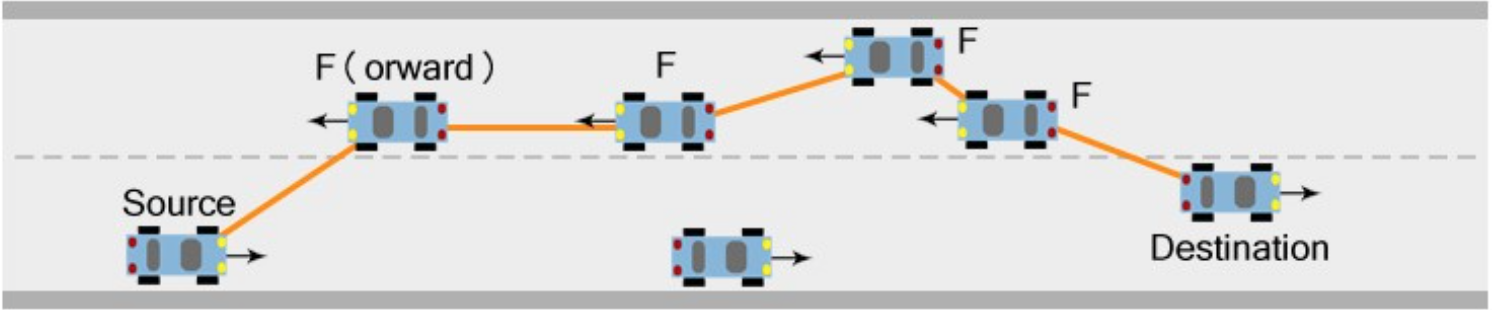
\includegraphics[width=0.99\textwidth]{content/images/03_networklayer/GeoUnicast.png}
	\caption{Geo Unicast \cite{etsi102636-1}}
	\label{fig:geounicast}
\end{figure}

\subsection{Topologically-scoped broadcast}
Der Topologically-scoped broadcast sendet einen Nachricht mit einem bestimmten Hop Count an alle um den Knoten erreichbaren Einheiten. Diese Nachricht wird dann von den Knoten empfangen, bei denen der Hop Count endet.

\begin{figure}
	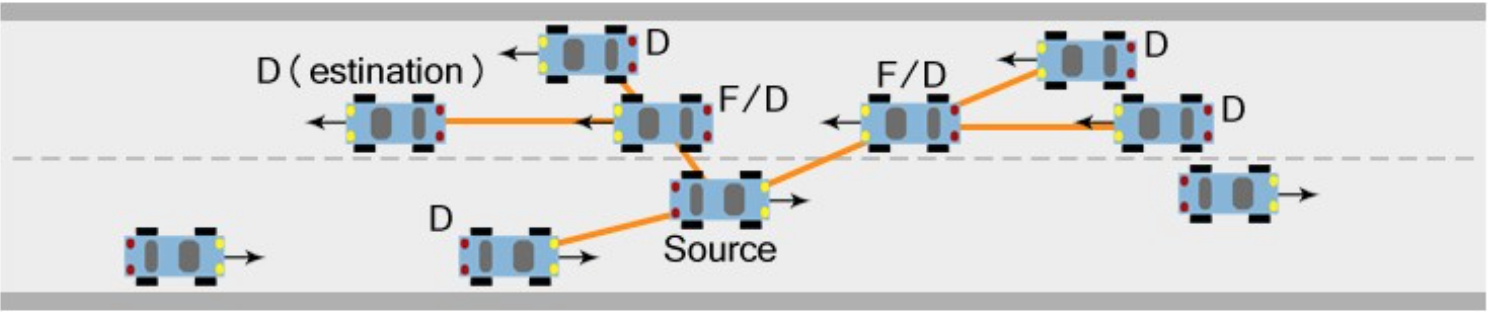
\includegraphics[width=0.99\textwidth]{content/images/03_networklayer/TSC.png}
	\caption{Topologically-scoped broadcast mit Hop Count 2 \cite{etsi102636-1}}
	\label{fig:tsc}
\end{figure}


\subsection{Geographically-scoped broadcast}
Über den Geographically-scoped broadcast ist es einem Knoten möglich, um sich herum oder in einer bestimmten Entfernung zu sich selbst eine definierte Region zu erreichen. Dabei spielt die Anzahl der Hops keine Rolle und alle in dem Bereich liegenden Fahrzeuge sollen sich angesprochen fühlen.

\begin{figure}
	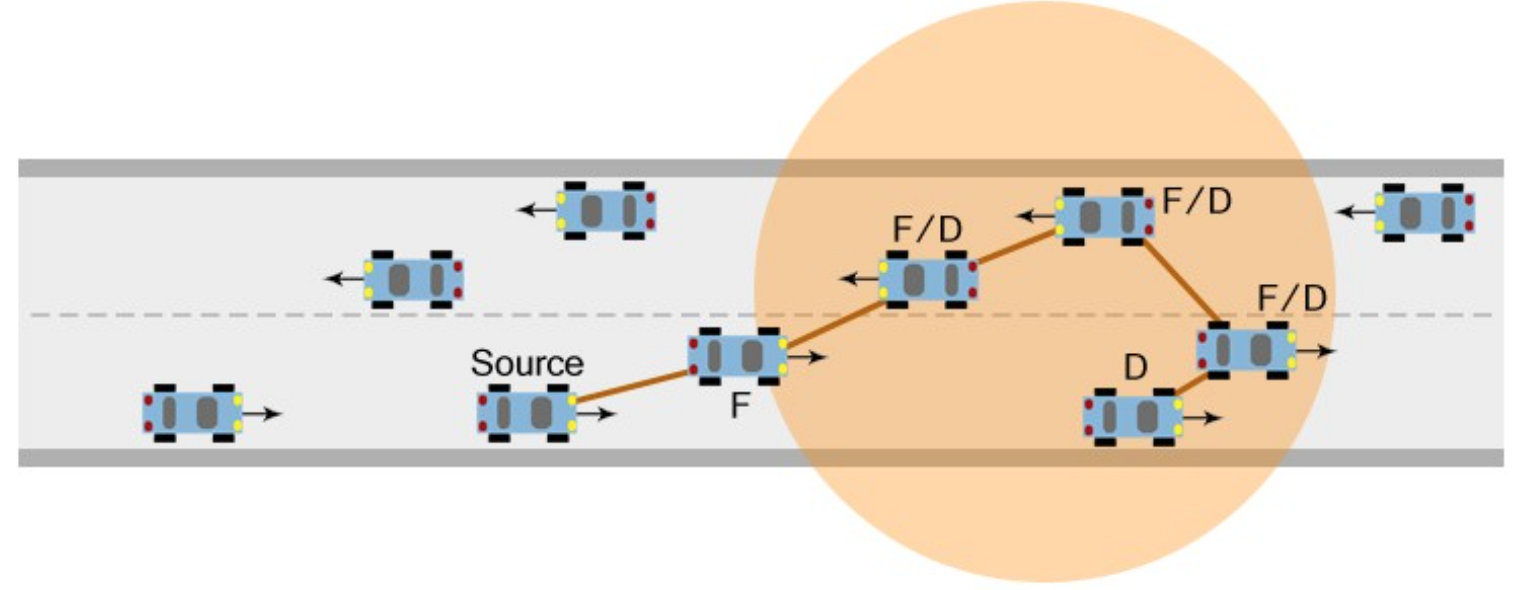
\includegraphics[width=0.99\textwidth]{content/images/03_networklayer/GSB.png}
	\caption{geographically-scoped broadcast \cite{etsi102636-1}}
	\label{fig:gsb}
\end{figure}

\subsection{Geographical Scoped Anycast}
Der Geographical Scoped Anycast ist ähnlich zu dem Geographically-scoped broadcast nur das hier die Nachricht nicht weitergeleitet wird sondern das Routing stoppt sobald ein Ziel innerhalb der Region die Nachricht empfangen hat.

\begin{figure}
	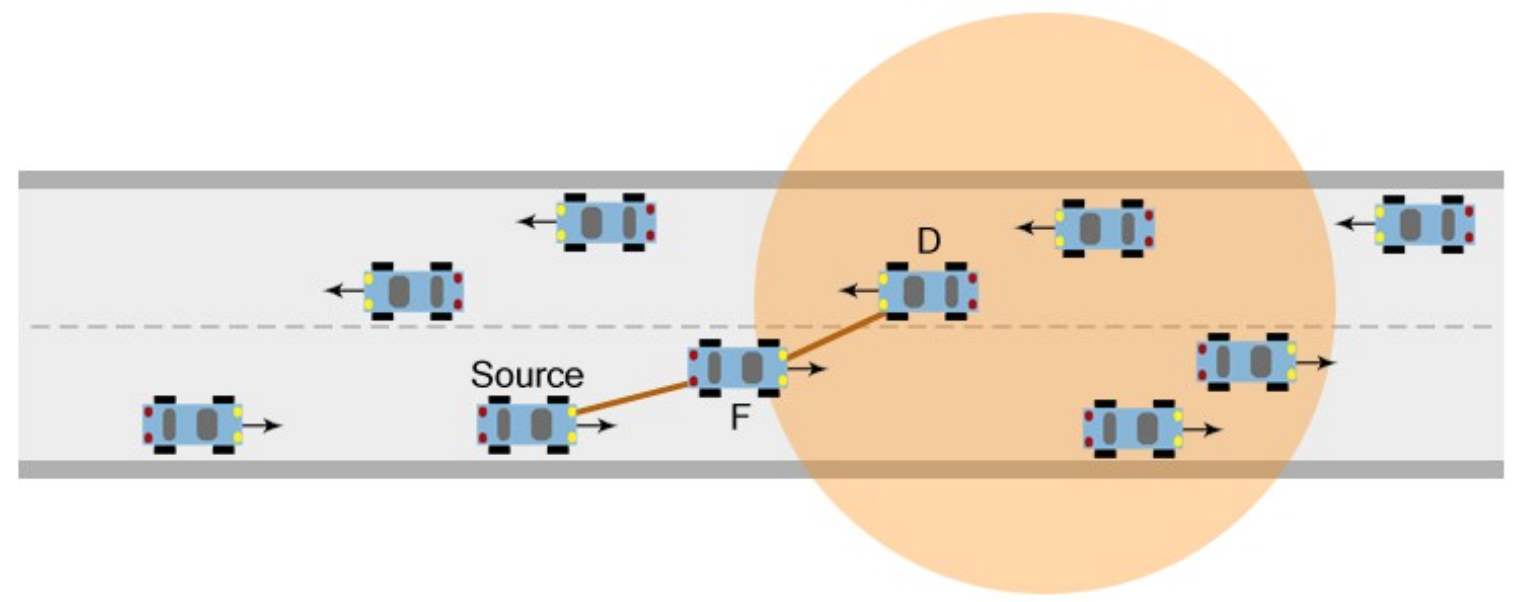
\includegraphics[width=0.99\textwidth]{content/images/03_networklayer/GSA.png}
	\caption{geographically-scoped anycast \cite{etsi102636-1}}
	\label{fig:gsa}
\end{figure}


	\chapter{Facility Layer \label{chap:facilitylayer}}
\section{Komponenten}
\begin{figure}[htbp]
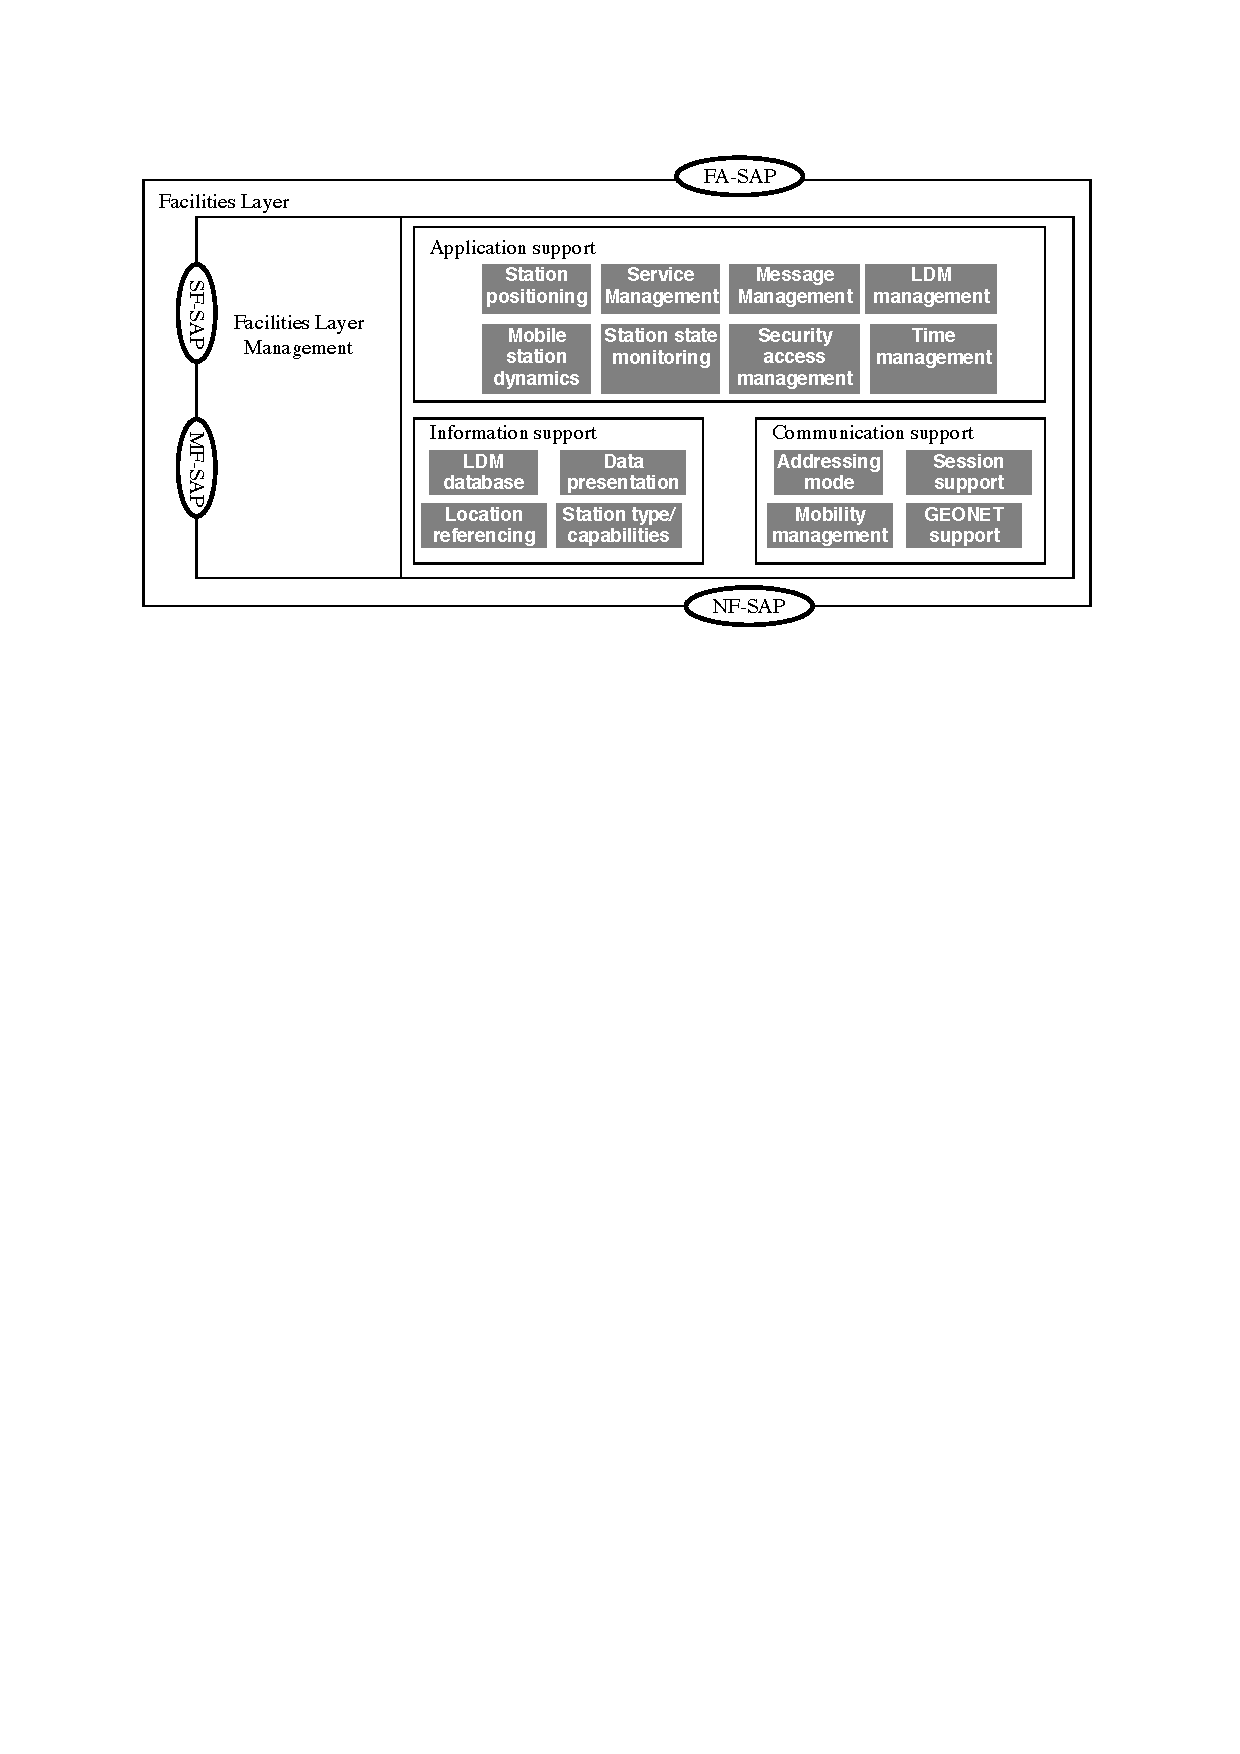
\includegraphics[width=0.99\textwidth]{content/images/04_facilitylayer/facility_layer_model.pdf}
\caption{Die Komponenten der \acl{C2C}}
\label{fig:komponentenfacility}
\end{figure}
Der Facility Layer liegt unterhalb des Applicationlayer und teilt sich in drei Hauptkomponenten auf. Er bietet verschiedene allgemeine Services an die von den Anwendungen des Application Layer verwendet werden können.

\subsection{Application Support}
Der Application Support stellt die Grundfunktionalität für die Anwendungen zur verfügung. Darunter fällt das station lifecycle management, das automatische erkennen von Services sowie das downloaden und initialisieren von neuen Services und noch weitere. Die einzelne Komponenten des Application Support, die auf der \autoref{fig:komponentenfacility} zu sehen sind, werden im folgenden genauer erläutert. 

\subsubsection{Station positioning}
Dieser teil des Application Support verarbeitet die Informationen die aus den verschiedenen Datensammler gewonnen werden wie aus GNSS oder aus Fahrzeugsensoren um die Position des Station zu gewinnen. 
Da diese Angaben sehr genau sein müssen werden die Daten in 3D Position gemessen (latitude, longitude, altitude). Dies können, durch beispielsweise GPS, in Echtzeit zur verfügung stehen. Da es jdeoch Sicherheitsbedingte Anwendungen gibt bei denen bereits über 0.5m Abweichung eine fatale Auswirkung haben kann, werden die Standortinformationen noch einmal über weitere Einheiten verbessert. Dazu gehören z.b. Odometer oder Gyroskop.
Damit diese Support facility ihren Aufgaben Nachkommen kann, ist im \cite{etsi102638} folgende Vorraussetzungen definiert.

\begin{itemize}
\item Benötigt Verbindung zwischen ITS station und einem GNSS system. Bei kurzfristigen Ausfall der Verbindung übernehmen interne mechanische Fahrzeugsensoren wie das Gyroskop oder das Odometer.
\item Benötigt dauerhafte Verbindung zu den Fahrzeugsensoren (direkte Verbindung oder über einen Bus).
\item Benötigt genug Rechenleistung um 3D Positions Angaben sicher zu Verwalten und zu Berechnen.
\end{itemize}

\subsubsection{Mobile station dynamic monitoring}
Das Mobile station dynamic monitoring ist nur für die \acs{VS} verfügbar. Diese Einheit des Facility Layer verwaltet eine große Anzahl an Fahrzeugspezifischen Daten die von den Applicationen und anderen Komponenten des Facility Layers verwendet werden. Sie ist dafür verantwortlich diese Daten immer auf dem neueste  Stand zu halten. 

\begin{itemize}
\item Benötigt zugriff auf Fahrzeug Funktionen wie das Bremssystem, Reifendruck, Stabilitätskontrolle, Geschwindigkeitsregelung etc.
\item Benötigt 
\item Benötigt genug Rechenleistung um 3D Positions Angaben sicher zu Verwalten und zu Berechnen.
\end{itemize}Diese Einheit benötigt die folgenden Vorraussetzungen.



This support facility requires access to vehicle functions according to selected options (e.g. braking system,
steering system, tyre pressure monitoring system, stability control system, speed control, etc.).
• This support facility requires capabilities to filter the selected parameters being needed by applications and
other facilities (e.g. master cylinder pressure, steering wheel angle, steering wheel angle rate of change,
programmed speed control value, stability control status, yaw rate, vehicle speed, acceleration control, etc.).
• This support facility requires capabilities to update parameters values being used for CAM. 


\subsubsection{Station state monitoring \label{facilitylayer_StationStateMonitoring}}
tr 102 638
\subsubsection{Services management \label{facilitylayer_ServicesManagement} }
tr 102 638
\subsubsection{LDM management \label{facilitylayer_LDMManagement}}
tr 102 638
\subsubsection{Messages management \label{facilitylayer_MessagesManagement}}
tr 102 638
\subsubsection{Security access management \label{facilitylayer_AccessManagement}}
tr 102 638
\subsubsection{Time management \label{facilitylayer_TimeManagement}}
tr 102 638
\subsubsection{Time management}
tr 102 638
\subsubsection{Time management}
tr 102 638
\subsection{Information Support}
The information support covers the presentation layer of the OSI reference model and holds the role of
data management. In any ITS system, there will be an abundance of data sources, both mobile and static
ones. These data will mostly be location referenced, time specific and attached with life time value and
with accuracy and reliability parameters. Therefore, fusing data and keeping the information up to date is
one of the challenges of information support. Main entity that supports this is Local Dynamic
Map (LDM) that is able to take data both from different sources and from received ITS messages to build
a data model of the local environment. Furthermore, the information support takes on many functions of
the OSI Presentation Layer. 
\subsubsection{LDM database}
\subsubsection{Data presentation}
\subsubsection{Location referecing}
\subsubsection{Station type/capabilities}

\subsection{Communication Support}
The communication support, which includes the session layer of the OSI Reference model. It will
cooperate with the transport and network layer to achieve the various communication modes required by
the applications. 

\section{CAM\label{sec:cam}}
\ac{ITS} bietet die Möglichkeit, dass \ac{ITS-S} untereinander Statusinformationen austauschen. Für den Austausch von Statusinformationen werden \ac{CAM} versandt. Diese beinhalten Informationen über die Anwesenheit allgemein, über die Position und den grundsätzlichen Status. Gemäß Standard \cite{ts102637-2} soll jede \ac{ITS-S} den Umgang mit diesen Nachrichten beherrschen. Das beinhaltet das Senden, das Empfangen und das Generieren dieser Nachrichten. So kennt jede \ac{ITS-S} ihre aktuellen Nachbarn inklusive ihrer Positionen, Bezwungen und den grundlegenden Sensorinformationen. Die \ac{CAM} werden über den Standard \ac{ITS-G5} übertragen. \ac{CAM} werden mit einer Kadenz zwischen 1 und 10 Hz übertragen, das bedeutet, dass mindestens jede Sekunde eine \ac{CAM} generiert und versendet wird, maximal werden aber 10 \ac{CAM} pro Sekunde generiert und versendet. Der Versand erfolgt über ein Single Hop Broadcast. \ac{CAM} spielen besonders für \ac{IVS} eine Rolle.

Die Verwaltung der \ac{CAM} findet im \ac{CAM} Management statt. Es hat Interfaces zu den anderen Facilities:
\begin{itemize}
	\item Station State Monitoring, \autoref{facilitylayer_StationStateMonitoring} (Bietet den aktuellen Staus der \ac{ITS-S} an)
	\item Mobile Station Dynamic Monitoring (Bietet Echtzeitkinematik der \ac{ITS-S} an)
	\item Time Management, \autoref{facilitylayer_TimeManagement} (Bietet eine global gültige Zeitreferenz für das markieren von Nachrichten an)
	\item Local Dynamic Map Management, \autoref{facilitylayer_LDMManagement}
\end{itemize}

Die anderen Facilities sind in der \autoref{fig:komponentenfacility} eingezeichnet. 

Das Nennen des vollständigen Inhalts einer \ac{CAM} würde den Rahmen dieser Ausarbeitung sprengen. Im Folgenden werden dennoch einige interessante Datenelemente aufgezählt. Sie entstammen dem Standard \cite{ts102637-2}. Dort können auch die Restlichen nachlesen werden.

\begin{itemize}
	\item \textbf{stationCharacteristics: } Dieses Datenelement besteht laut der \ac{ASN.1} Beschreibung aus mindestens drei weiteren Datenelemten:
	\begin{itemize}
		\item mobileItsStation: Kann die \ac{ITS-S} ihre Station ändern?
		\item privateItsStation: Die \ac{ITS-S} wird von keiner Behörde betrieben.
		\item physicalRelevantItsStation: Kann eine andere \ac{ITS-S} diese \ac{ITS-S} rammen?
	\end{itemize}
	\item \textbf{AmbientAirTemperature: } Die Außentemperatur, die die \ac{ITS-S} misst.
	\item \textbf{CrashStatus: } Dieses Datenelement enthält Informationen über einen Unfall, der eine Weiterfahrt verhindert. Beispiele dafür sind das Auslösen der Airbags oder ein Überschlag.
	\item \textbf{CurvatureChange: } Dieses Datenelement beschriebt die Änderung der Kurvenrichtung. Ein positiver Wert bedeutet, dass das \ac{IVS} nach rechts abbiegt.
	\item  \textbf{DangerousGoods: } Dieses Datenelement beschreibt, ob und welches Gefahrgut  das \ac{IVS} transportiert.
	\item \textbf{StationWidth: } Dieses Element beschreibt die zulässige Gesamtbreite der \ac{ITS-S}. Die Breite ist mit einer Feinheit von 0,01m aufgelöst.
\end{itemize}


\section{DEN\label{sec:den}}
\ac{DEN} ist definiert um die \ac{RHW} Anwendungsfälle zu unterstützen.	Die \ac{RHW} Anwendung ist auf \ac{IVS} und \ac{ITS} verteilt. Sie ist eine aktive Straßensicherheit Anwendung. Sie verteilt Informationen über die Straßenverkehrsverhältnisse. Um die \ac{DEN} Informationen zu verteilen gibt es \ac{DENM}. Diese enthalten die relevanten Informationen und informieren die andren \ac{ITS-S}. Sie werden beim Eintreffen eines \ac{RHW} relevanten Ereignisses an alle \ac{ITS-S} verteilt, die durch dieses Ereignis betroffen sind. Während das Ereignis anhält, werden die \ac{DENM} verteilt. Das Verteilen endet nach einer festgelegten Zeit oder durch eine weitere \ac{DENM}, die eine andere beendet. In einer \ac{ITS-S}, die eine \ac{DENM} empfängt, wird geprüft, ob die Information für den Benutzer relevant ist. Abhängig der Relevanz wird sie angezeigt oder nicht. Ein Beispiel für eine \ac{DENM}, die nach einer festen Zeit ungültig wird, ist eine Notbremsung eines \ac{IVS}. Durch die Bremsung entsteht eine temporäre Gefahr. 


\section{SPaT\label{sec:spat}}
\ac{SPaT} ist eine Nachricht, die den Zustand einer Straßenkreuzung beschreibt. Die Beschreibung enthält Staus Informationen der \ac{VBA} und Informationen über die Kreuzung selber. \ac{SPaT} ist noch nicht von der \ac{ETSI}, bzw. \ac{ISO} standardisiert. Aus diesem Grund stammen die folgenden Informationen hauptsächlich aus den U.S. amerikanischen Quellen \cite{usSpat} und \cite{usCaliforniaSpat}. 

Für \ac{SPaT} gibt es zwei grundsätzliche Betriebsarten. Die erste Betriebsart ist eine feste \ac{VBA} Schaltung. Diese wird den \ac{IVS} über \ac{SPaT} Nachrichten mitgeteilt. Anhand dieser Informationen kann das \ac{IVS} selber die Ampelzeiten berechnen und benötigt keine  weiteren \ac{SPaT} Nachrichten. Die zweite Betriebsart ist, dass die Ampelzeiten aufgrund externer Ereignisse beeinflusst werden können. Externe Ereignisse sind beispielsweise Fußgänger, verkehrsabhängige Schaltungen oder periodisierte \ac{IVS}, wie z.B. Rettungswagen. Bei der zweiten Betriebsart muss beachtet werden, dass zu schnelle Änderungen vermieden werden müssen. Die \ac{IVS} benötigen eine bestimmte Zeit zur Reaktion, so benötigt beispielsweise ein Auto die Reaktionszeit des Fahrers und einen Bremsweg. Wird die Fahrspur dieses Autos gesperrt und andere Fahrspuren dafür freigegeben, wenn das Auto sich schon fast vor der Haltelinie befindet, so ist eine Bremsung vor der Kreuzung nicht mehr möglich. Daraus resultiert ein Sicherheitsrisiko, da die andere Fahrspur nicht für die anderen Fahrzeuge garantiert frei ist. \todo{Rausfinden, ob die \ac{IRS} die Position des \ac{IVS} verwertet und daraus die Zeiten generiert. S.29 US Department.. -> Ich glaube die verwendet die Daten}

Auf dieser Grundlage können weitere Dienste angeboten werden. So können Abbiegeassistent Systeme oder Vorzugsschaltungen realisiert werden. 

 Abbiegeassistent Systeme unterstützen \ac{IVS} beim Abbiegen in Kreuzungen. Anhand der Positions- und Geschwindigkeitsdaten der \ac{IVS} kann die \ac{IRS} berechnen, ob ein Abbiegen nach rechts oder nach links sicher ist. Neben der Positionsdaten können auch Erfassungssysteme genutzt werden, die in die Infrastruktur integriert sind. Beispiele hierfür können \ac{Radar} oder \ac{Lidar} Systeme genutzt werden. Der Nachteil von rein \ac{ITS} basierten Systemen ist, dass nicht \ac{ITS} kompatible Fahrzeuge nicht erkannt werden. Das bedeutet, dass die \ac{IRS} eine freie Kreuzung erkennt und meldet, obwohl nicht \ac{ITS} basierende Fahrzeuge über die Kreuzung fahren. 
 
Die Bevorzugung von Fahrzeugen bietet sich für die Empfehlung \cite{usSpat} für Notfallfahrzeuge, für Fahrzeuge des Nahverkehrs und für den Frachtverkehr an. Durch die Bevorzugung können diese \ac{IVS} eine grüne Welle erreichen. Das bedeutet, dass entweder Grünphasen verlängert werden oder Rotphasen unterbrochen werden. Sofern nicht bereits durch andere Nachrichten, wie \ac{CAM} geschehen, fordert das \ac{IVS} bei der \ac{IRS} eine Bevorrangung an, wenn anhand der \ac{SPaT} erkennt, dass die Kreuzung nicht frei ist. Die \ac{IVS} beantwortet diese Anfrage im positiven Fall mit einer weiteren \ac{SPaT} Nachricht, die eine freie Kreuzung signalisiert.   

Inhalt einer \ac{SPaT}:
\begin{longtable}{|c|c|}
 \hline
\textbf{Datenelemente} & \textbf{Typ/Größe}\\
 \hline
 \hline
Object ID & Unsigned 8 Bit Integer\\
 \hline
 Object Size& Unsigned 8 Bit Integer\\
 \hline
 Apptoach ID & Unsigned 8 Bit Integer\\
 \hline
 Signal Phase Indication &  32 Bit Bitmask \\
 \hline
 Countdown Timer Confidence & 32 Bit Bitmask \\
 \hline
 Time to Signal Phase Change (Countdown Time) & Unsigned 16 Bit Integer \\
 \hline
 Yellow Duration & Unsigned 8 Bit Integer\\
 \hline
 \caption{Inhalt einer SPaT Nachricht \cite{usSpat}}
 \label{tab:facilitylayer_inhaltSpatNachricht}
 \end{longtable}
 
\todo{Werte der Tabelle beschreiben oder den Mist löschen}
\begin{figure}[htbp]
	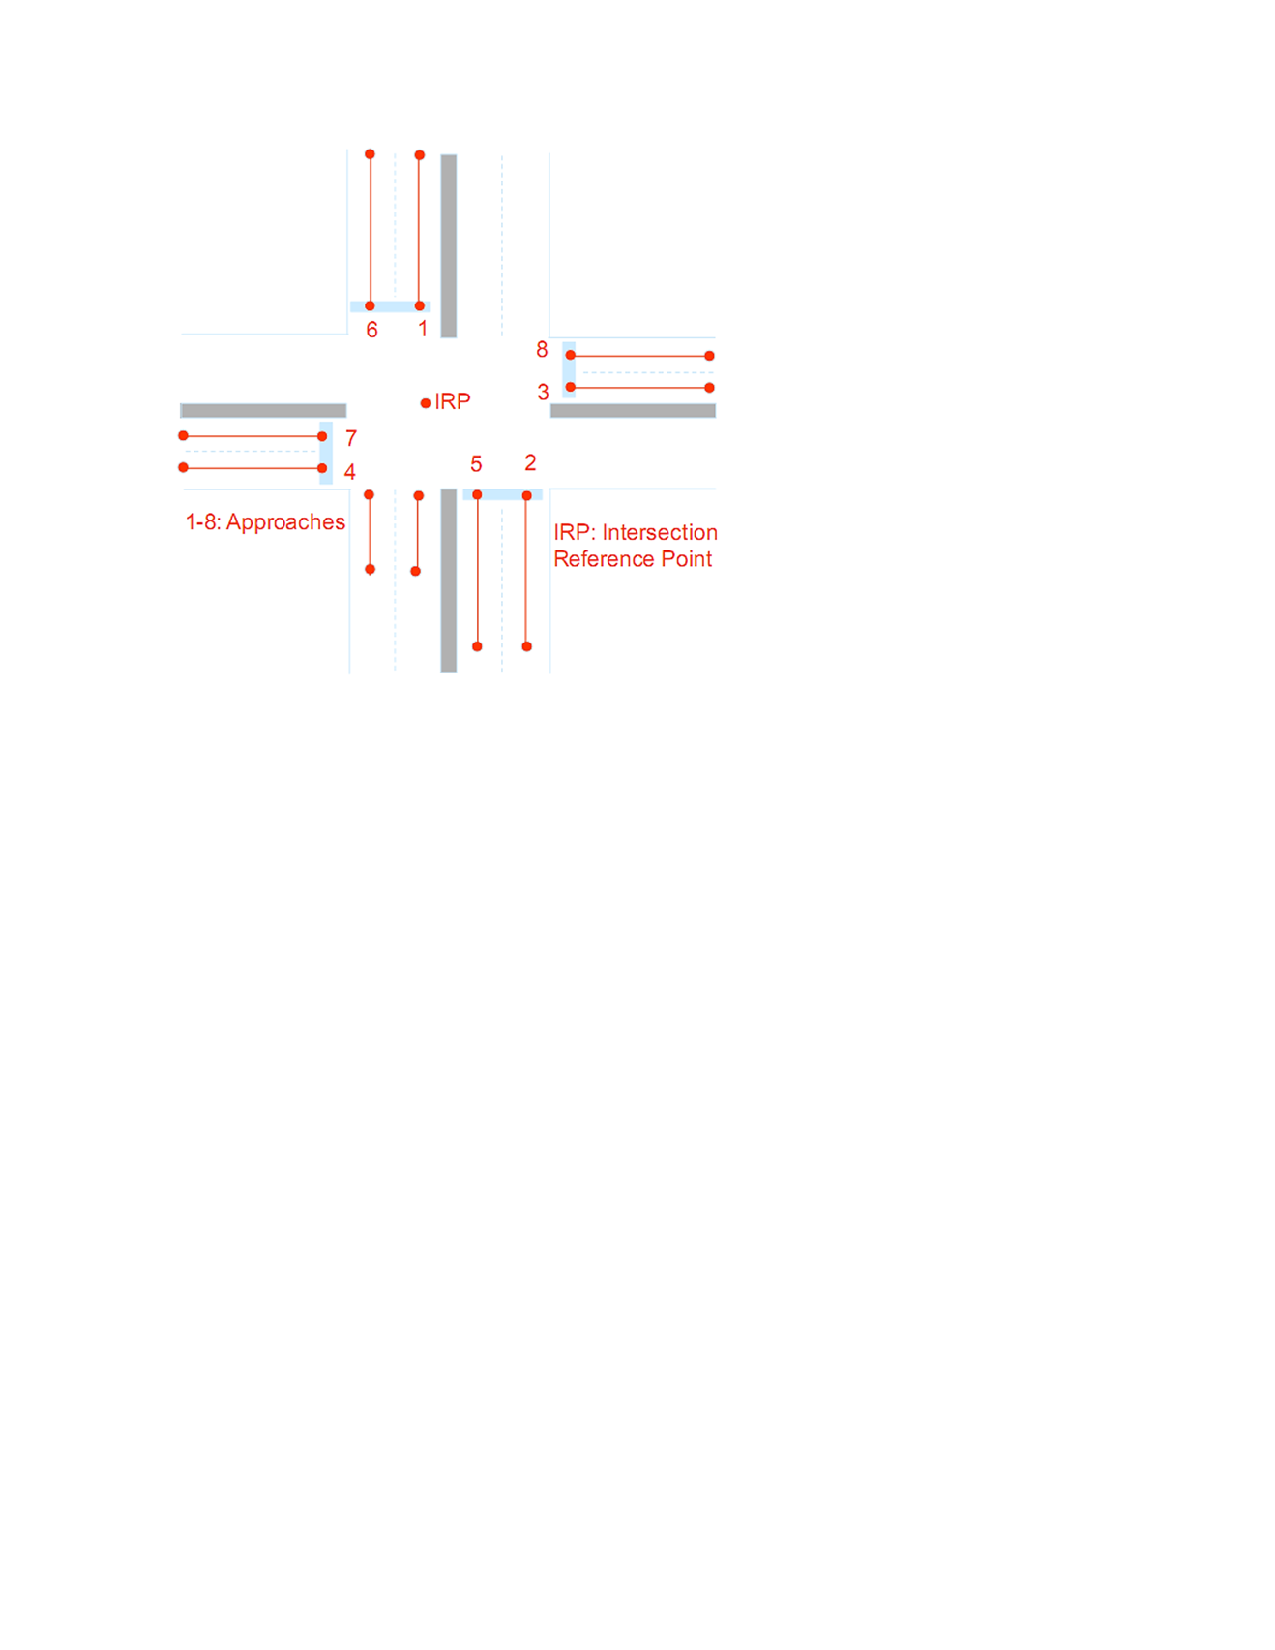
\includegraphics[width=0.60\textwidth]{content/images/04_facilitylayer/spatKreuzung-Anfahrtsstreifen.pdf}
	\caption{Kreuzung mit Darstellung der Approach ID \cite{usSpat}}
	\label{fig:darstellungKreuzung}
\end{figure}




\section{TOPO\label{sec:topo}}

	\chapter{Application Layer\label{chap:applicationlayer}}


	\chapter{Application layer und Use Cases\label{chap:usecases}}
\section{Application Layer \label{sec:applicationLayer}}
\begin{figure}[htbp]
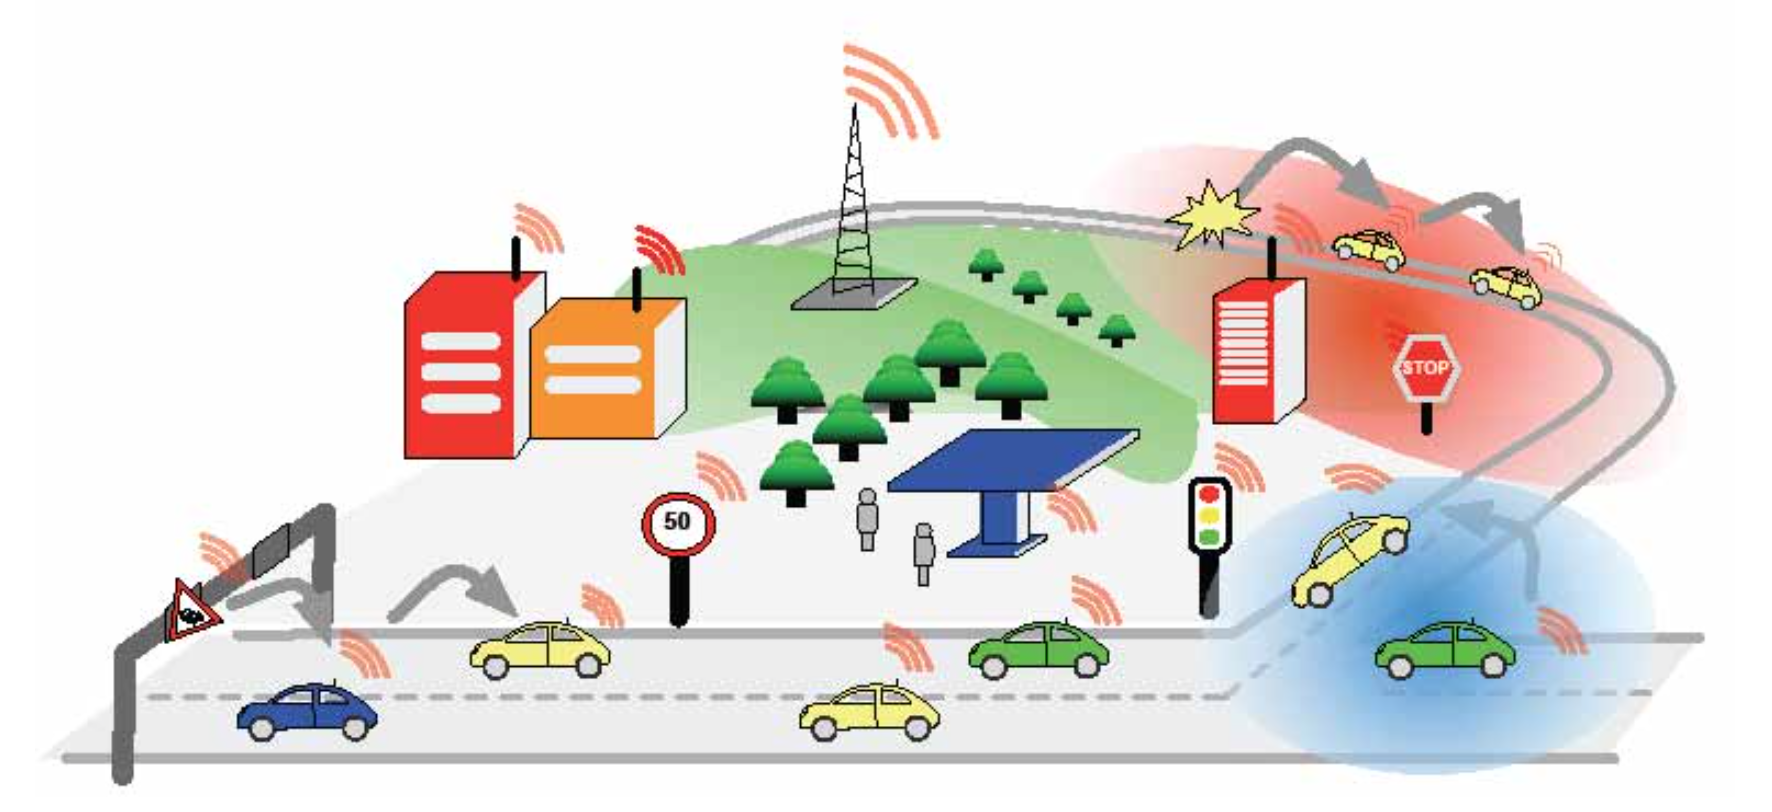
\includegraphics[width=0.99\textwidth]{content/images/06_use_cases/komponenten.png}
\caption{Die Komponenten der \acl{C2C}\cite{etsi102638}}
\label{fig:komponentenderc2x}
\end{figure}
Die \acl{C2C} bietet eine große Vielfalt an verschiedenen Einsatzmöglichkeiten. Da es sich bei dem gesamten Projekt nicht nur darum handelt das Fahrzeuge untereinander kommunizieren, sondern wie auf \autoref{fig:komponentenderc2x} zu sehen, auch andere Verkehrskomponenten. Um das Zusammenspiel der Komponenten besser zu verstehen und zu sehen wie groß das Potential der \acl{C2C} ist, werden im folgenden mehrere Szenarien aufgezählt und erklärt. Der Applicaationlayer unterscheidet dabei drei Kategorien von Anwendungsfällen. Dazu gehören die Sicherheitsbedingten, die Verkehrseffizienz und die Kategorie Infotainment und andere.

\section{Use cases}
\subsection{Sicherheitsbedingt}
Sicherheitsbedingte Szenarien sind Fälle bei denen ein Möglicher Unfall verhindert werden kann. Im Folgenden werden drei Szenarien erklärt bei denen das Unfallrisiko minimiert werden kann.

\subsubsection{Cooperative Forward Collision Warning}
Einer der häufigsten Ursachen für Verkehrsunfälle sind plötzliche Bremsmanöver von Vorrausfahrenden Fahrzeugen und die Unaufmerksamkeit eines Fahrers. Aus diesen Ursachen besteht ein erhöhtes Risiko für Auffahrunfälle. Cooperative Forward Collision Warning versucht genau dieses Risiko zu vermindern. Um dies zu vollbringen überwacht jedes Fahrzeug die eigenen Informationen, wie die Geschwindigkeit, Richtung und Position und vergleicht diese mit den Daten der anderen Fahrzeugen. Bei Auffälligkeiten und Abweichungen warnt das System dem Fahrer frühzeitig vor einer möglichen Kollision. Diese Warnung kann durch auditive, visuelle oder haptische Alarme signalisiert werden. Da es durchaus sein kann das noch Fahrzeuge, die nicht in dem C2C Netz kommunizieren, unterwegs sind, können über Objekterkennungssensoren diese ebenfalls identifiziert werden. Dadurch sinkt das Risiko noch einmals für die C2C Teilnehmer. Die Informationen werden innerhalb von 20 bis 200 meter geteilt womit auch genug Zeit bleibt um diese Auszuwerten und den Fahrer frühzeitig zu Informieren. \\
Nachfolgend wird gezeigt wie die Use Cases im Standart definiert werden. Dazu solle dieses Beispiel noch einmal dienen.

\textbf{Application name:} Co-operative collision avoidance or mitigation.
\textbf{Short description:} This use case is based on co-operation between vehicles which detect a risk of forward collision.
Such co-operation is achieved to avoid accident either through driver assistance of direct action on the cars.
\textbf{Usage:} Avoid longitudinal collision.
\textbf{Communication mode:} V2X co-operative awareness associated to unicast.
\begin{figure}[htbp]
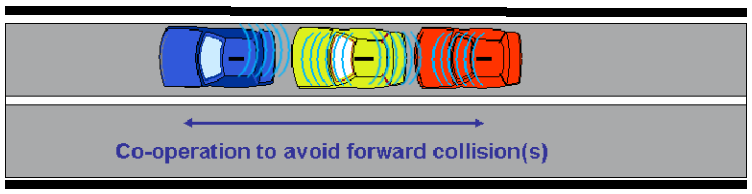
\includegraphics[width=0.99\textwidth]{content/images/06_use_cases/colissionwarning.png}
\caption{Cooperative Forward Collision Warning Use Case\cite{etsi102638}}
\label{fig:cfcw}
\end{figure}
\textbf{Main requirements}
\begin{itemize}
\item Capability for a vehicle to broadcast V2X co-operative awareness messages.
\item Capability for this vehicle to establish unicast Peer to Peer sessions to co-operate with other vehicles closely
\item Maximum latency time: 100 ms.
\item Minimum frequency of V2V co-operation awareness messages: 10 Hz.
\item Authenticity of V2X co-operative awareness messages.
\item Vehicles relative positioning accuracy: < 1 m.
following the same path to reduce the risk of accident.
\end{itemize}

\subsubsection{Pre-Crash Sensing/Warning}
Natürlich können nicht alle Unfälle durch die Cooperative Forward Collision Warning vermieden werden. Daher ist davon auszugehen das dennoch Auffahrunfälle geschehen werden. Dafür hat man sich das Pre-Crash Sensing/Warning Szenario ausgedacht, bei dem man von einem Unvermeidbaren Unfall ausgeht. Dies soll durch die \acl{C2C} erkannt und Vorbereitungen für den Unfall getroffen werden. Damit dieses System funktioniert muss wie bei dem vorherigen Szenario dauerhaft Informationen der Fahrzeuge ausgetauscht werden. Dabei geht man davon aus das die Informationen der Fahrzeuge die sich im Umkreis von 20 bis 100 meter befinden überwacht werden müssen. Entdeckt das System einen unvermeidbaren Unfall muss sichergestellt sein das diese Fahrzeuge die Kollidieren werden sicher miteinander kommunizieren können um Daten wie die, Fahrzeuggröße und genaue Position bekannt zu geben. Über diese Informationen können dann Sicherheitsmaßnahmen wie Airbar, Gurtstraffer oder erweiterbare Stoßstangen gesteuert werden und effektiv genutzt werden. 
\begin{figure}[htbp]
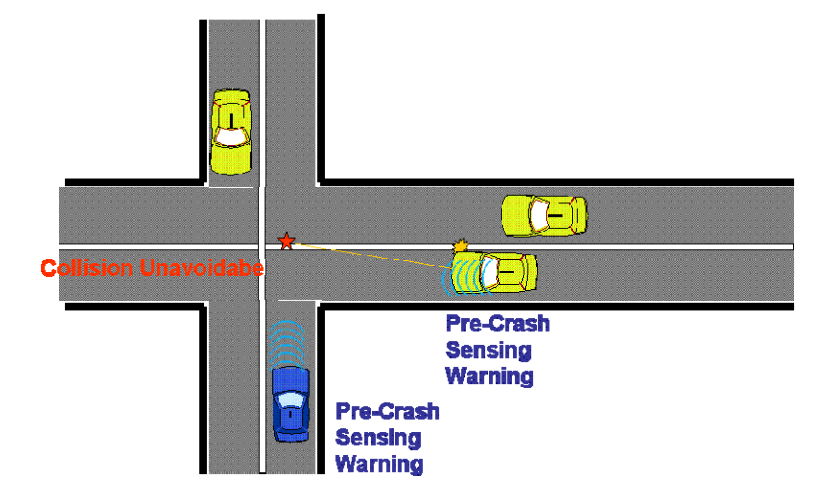
\includegraphics[width=0.99\textwidth]{content/images/06_use_cases/pre_crash_sensing.png}
\caption{Pre-Crash Sensing/Warning Use Case\cite{etsi102638}}
\label{fig:pcs}
\end{figure}
\subsubsection{Hazardous Location C2C Notification}
Die Hazardous Location C2C Notification soll dafür sorgen das gefährliche Fahrpassagen weitergegeben werden. Das heisst das System warnt nachkommende Fahrzeuge vor glatten Straßen oder Schlaglöchern. Die Schwierigkeit hierbei ist die Gewinnung der Informationen. Als Beispiel wird genannt das ein Fahrzeug das auf einer glatten Straße fährt und das ESP einsetzt, speichert an welcher stelle, Geschwindigkeit etc. eingetreten ist und diese Nachricht dann weiter sendet. Fahrzeuge die diese Warnnachricht erhalten können dann auf den Umstand mit Verbesserung der Sicherheitsmaßnahmen reagieren oder zumindest dem Fahrer darüber Informieren. 
\begin{figure}[htbp]
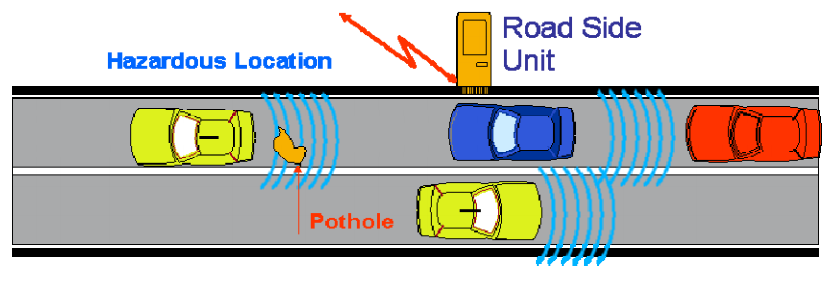
\includegraphics[width=0.99\textwidth]{content/images/06_use_cases/hln.png}
\caption{Hazardous Location C2C Notification Use Case\cite{etsi102638}}
\label{fig:hln}
\end{figure}

\subsection{Verkehrseffizienz}
Die Effizienz zu des Verkehrs zu steuern ist der ursprüngliche Sinn der \acl{C2C}. Durch die bessere Leitung des Verkehrs entstehen weniger Staus auf den Straßen, was zu verminderten Stresssituationen für Fahrer führt. Dadurch entstehen verkürzte Wartezeiten für die Teilnehmer am Verkehr und geringere Wartungskosten für die Straßen. Ausserdem kann dadurch die Umwelt mehr geschont werden und die Energiekosten sinken. 

\subsubsection{Enhanced Route Guidance and Navigation}
Navigation ist ein großes Thema das bereits über Navigationssysteme stark verbessert wurde. Enhanced Route Guidance and Navigation soll die Navigation noch einmal verbessern. Dies soll erreicht werden in dem die Fahrdaten von den Roadside Stations gesammelt und ausgewertet werden. Dadurch können Verkehrsaufkommnisse vorhergesagt werden und Fahrzeuge auf ihrem Weg an einer solche Station vorbeikommen können über die aktuellen Verkehrsinformationen aufgeklärt werden und den effektivsten Weg berrechnen um die Verkehrsdichte zu verbessern. Damit dieses Szenario funktioniert müssen die Roadside Stations die Möglichkeit besitzen vorbeifahrende Fahrzeuge zu erkennen und zu Informieren. 
\begin{figure}[htbp]
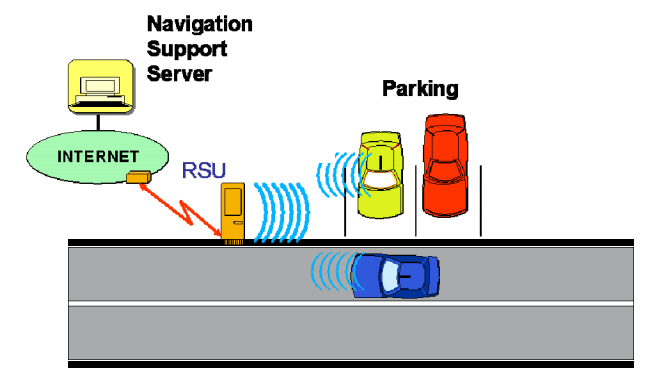
\includegraphics[width=0.99\textwidth]{content/images/06_use_cases/ergn.png}
\caption{Enhanced Route Guidance and Navigation Use Case\cite{etsi102638}}
\label{fig:ergn}
\end{figure}
\subsubsection{Green Light Optimal Speed Advisory}
Green Light Optimal Speed Advisory beschäftigt sich mit der optimalen Geschwindigkeit zwischen Ampeln. Damit Fahrzeuge zwischen Ampelabschnitten nicht die Geschwindigkeit reduzieren und nach Möglichkeit nicht immer wieder neu Anfahren müssen, kann durch eine Kreuzung die an der \acl{C2C} teilnimmt Informationen über die Rot-Grün Schaltzeit eingeholt werden. Über den bekannten Abstand zum vorherfahrenden Auto kann die optimale Geschwindigkeit berechnet werden, die das Fahrzeug sich vorwärts bewegen sollte um während einer Grünphase der Ampel dort einzutreffen. Dadurch wird der Verkehrsfluss verbessert und schont die Tankfüllung eines Autos.
\begin{figure}[htbp]
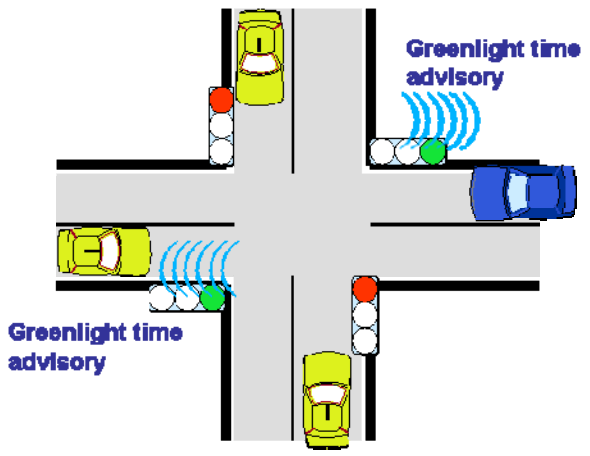
\includegraphics[width=0.99\textwidth]{content/images/06_use_cases/greenlight_opimalspeed.png}
\caption{Green Light Optimal Speed Advisory Use Case\cite{etsi102638}}
\label{fig:glos}
\end{figure}
\subsubsection{C2C Merging Assistance}
Bei einfahren in den Verkehr von kann es vorkommen das ein Fahrzeug den fliesenden Verkehr stört. Dadurch entstehen nicht selten Rückstaus die im schlimmsten Fall zu Auffahrunfällen führen. Dies soll über C2C Merging Assistance bereits beim einfahren in den fliesenden Verkehr verhindert werden, in dem das Fahrzeug das in den Verkehr einfliesen möchte die betroffenen Fahrzeuge darüber informiert. Die Fahrzeuge die betroffen sind sollen ihre ihre Geschwindigkeit automatisch reduzieren oder zumindest sollen die Fahrer darüber Informiert werden wie sie sich am besten Verhalten sollen. Dadurch kann der Verkehr weiter sauber fliesen ohne das es im Nachhinein zu einem stillstand kommt. 
\begin{figure}[htbp]
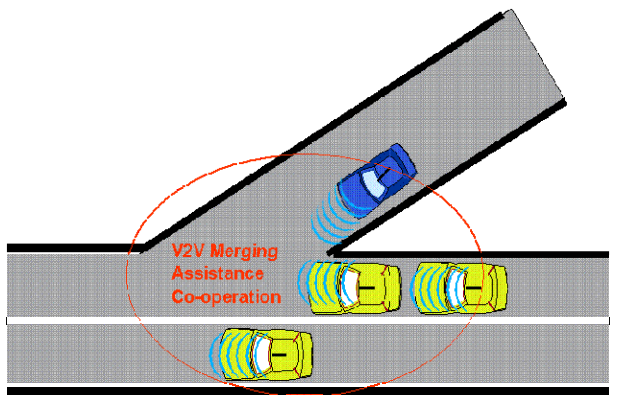
\includegraphics[width=0.99\textwidth]{content/images/06_use_cases/merging_assistance.png}
\caption{C2C Merging Assistance Use Case\cite{etsi102638}}
\label{fig:mergingassistance}
\end{figure}
\subsection{Infotainment und andere}
Hier werden die Anwendungsfälle aufgeführt die nicht zur Sicherheit oder Verkehrseffizienz beitragen aber dennoch über die \acl{C2C} realisiert werden. Dazu gehören allgemeine Informationen, Entertainment oder Fahrzeugdaten wie der Verbrauch reduziert werden kann. 
\subsubsection{Point of Interest Notification}
Dieser Anwendungsfall ist besonders für Kommerzielle Werbezwecke interessant. Hier werden durch eine Roadside Station Informationen über für den Fahrer interessante Orte zu den Umliegenden Fahrzeugen gesendet. Die Masse an Informationen kann durch das Fahrzeug gefiltert werden und immer Situationsbedingt die passenden Orte vorgeschlagen werden. Zum Beispiel wenn der Benzinstand des Fahrzeuges niedrig ist können die in der nähe befindlichen Tankstellen mit Öffnungszeiten und preise dem Fahrer vorgeschlagen werden. Dadurch wird die Werbung deutlich effektiver da die Zielgruppe richtig gewählt wird und sich in der unmittelbaren Umgebung aufhält.
\begin{figure}[htbp]
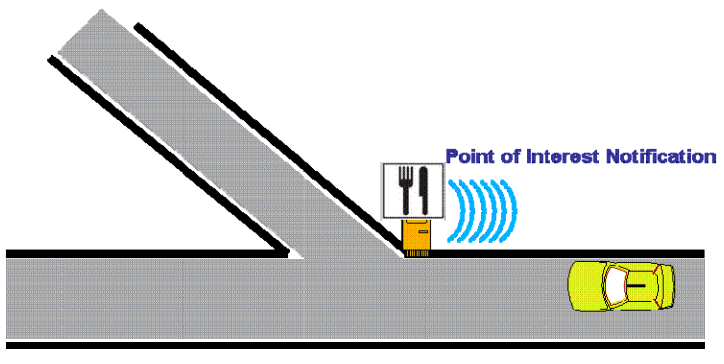
\includegraphics[width=0.99\textwidth]{content/images/06_use_cases/poin.png}
\caption{Point of Interest Notification Use Case\cite{etsi102638}}
\label{fig:poin}
\end{figure}
\subsubsection{Remote Diagnostics}
Der Remote Diagnostics Anwendungsfall beschreibt ein Szenario zum Warten des Autos ohne dafür in eine Werkstatt fahren zu müssen. Dadurch können Informationen über das Fahrzeug abgerufen werden und mit Hilfe der Problembeschreibung des Fahrers kann schnell festgestellt werden um was es sich handelt. Die Daten über Werkstattbesuche und was an dem Auto angefallen ist soll alles in eine Datenbank geschrieben werden sodass die Werkstatt die das Fahrzeug wartet immer weiss was gemacht worden ist. So wird die Zeit die für die Wartung eines Fahrzeuges reduziert und damit auch die Länge des Besuches in der Werkstatt für den Kunden. Um die Software eines Autos aktuell zu halten wird überhaupt kein Werkstattbesuch mehr benötigt, da das update direkt beispielsweise über das Internet geladen werden kann.
\begin{figure}[htbp]
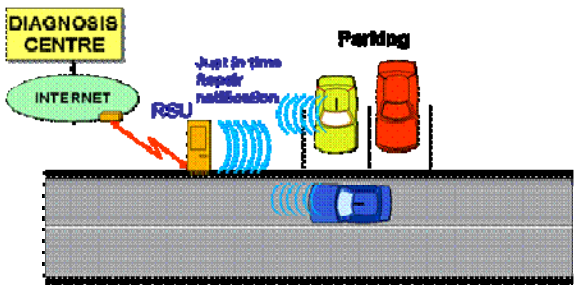
\includegraphics[width=0.99\textwidth]{content/images/06_use_cases/rds.png}
\caption{Remote Diagnostics\cite{etsi102638}}
\label{fig:redia}
\end{figure}

	



%Uebersicht über die Abkürzungen
\cleardoublepage
\addchap{Abkürzungsverzeichnis}
\label{abkuerzungsverzeichnis}
\begin{acronym}[LONGEST]
	
% In case that this file is empty and disabled in settings.tex, you can delete
% this file.
\acroplural{VBA}[VBA]{Verkehrsbeeinflussungsanlagen}
\acro{ABS} {Antiblockiersystem}
\acro{AKTIV} {Adaptive und Kooperative Technologien für den Intelligenten Verkehr}
\acro{ASN.1}{Abstract Syntax Notation One}
\acro{ASR} {Antriebsschlupfregelung}
\acro{AU}{Application Unit }
\acro{C2C-CC} {Car to Car Communication Consortium}
\acro{C2C} {Car-to-Car Kommunikation}
\acro{C2I} {Car-to-Infra\-structure Kommunikation}
\acro{C2X} {Car-to-X Kommunikation}
\acro{CABS} {Cooperative Awareness Basic Service}
\acro{CAM} {Cooperative Awareness Message}
\acro{CA}{Cooperative Awareness}
\acro{CCU}{Communication \& Control Unit}
\acro{CONVERGE} {COmmunication Network VEhicle Road Global Extension}
\acro{CS} {Central Server}
\acro{CTX}{Service Context Message}
\acro{CVIS} {Cooperative Vehicle-Infrastructure Systems}
\acro{DCC}{Decentralizied Congestion Control}
\acro{DENM} {Decentralized Environmental Notification Message}
\acro{DEN} {Decentralized Environmental Notification}
\acro{EDV}{Elektronische Datenverarbeitung}
\acro{EIRP} {Äquivalente isotrope Sendeleistung (engl. equivalent isotropically radiated power)}
\acro{ETSI-ITS} {European Telecommunications Standards Institute Intelligent Transportation Systems}
\acro{ETSI}{European Telecommunications Standards Institute}
\acro{FGVT} {Forschungsgruppe Verkehrstelematik}
\acro{FRAMES} {Frühwarnsystem zur Adaptiven Fahrzeug-Mensch-Erkennung und Sicherheitsförderung}
\acro{GAR}{GeoAdhoc router}
\acro{GBAS} {Ground-Based Augmentation System}
\acro{GNSS} {Global Navigation Satellite System}
\acro{GNW}{Geo Networking}
\acro{GPS} {Global Positioning System}
\acro{GSM} {Global System for Mobile Communications}
\acro{HTW} {Hochschule für Technik und Wirtschaft des Saarlandes}
\acro{ICS} {ITS Central Station}
\acro{ID} {Identifikator}
\acro{IEEE} {Institute of Electrical and Electronics Engineers}
\acro{IRS} {\ac{ITS} Roadside Station}
\acro{ISO}{International Organization for Standardization}
\acro{ITS-G5}{5 GHz wireless communication}
\acro{ITS-S}{\ac{ITS} Station}
\acro{ITS} {Intelligent Transportation Systems}
\acro{ITU-T}{International Telecommunication Union – Telecommunication Standardization Sector}
\acro{ITeM} {ITS Testfeld Merzig}
\acro{IVS} {ITS Vehicle Station}
\acro{KI} {Kommunikationsinformatik}
\acro{LDM}{Local Dynamic Map}
\acro{LKW} {Lastkraftwagen}
\acro{LSA} {Lichtsignalanlage}
\acro{LTE} {Long Term Evolution}
\acro{LWL} {Lichtwellenleiter}
\acro{LZA} {Lichtzeichenanlage}
\acro{Lidar} {Light detection and ranging}
\acro{Lidar}{Light detection and ranging}
\acro{MP}{Messpunkt}
\acro{NAVSTAR-GPS} {Navigational Satellite Timing and Ranging – Global Positioning System}
\acro{OBU} {On Board Unit}
\acro{OSGi} {Open Service Gateway initiative}
\acro{OSI}{Open System Interconnection}
\acro{PDA}{Personal Digital Assistant}
\acro{PLZ} {Postleitzahl}
\acro{PSS}{Personal Subsystem and Station}
\acro{PaaS} {Platform as a Service}
\acro{QGIS} {QuantumGIS}
\acro{RHW}{Road Hazard Warning}
\acro{RSU} {Roadside Unit}
\acro{RTK} {Real Time Kinematics}
\acro{Radar} {Radio Detection and Ranging}
\acro{Radar}{Radio Detection and Ranging}
\acro{SAM}{Service Advertisement Message}
\acro{SAP}{Service Access Point}
\acro{SBAS} {Satellite-Based Augmentation System}
\acro{SIMTD}[sim\textsuperscript{TD}]{Sichere Intelligente Mobilität Testfeld Deutschland}
\acro{SPaT} {Signal Phase and Time}
\acro{SPaT}{Signal Phase and Timing}
\acro{TMC} {Traffic Message Channel}
\acro{TOPO} {Topology Specification}
\acro{UMTS} {Universal Mobile Telecommunications System}
\acro{URBAN}[UR:BAN]{Urbaner Raum: Benutzergerechte Assistenzsysteme und Netzmanagement}
\acro{UTC}{Universal Time, Coordinated}
\acro{UUID} {Universally Unique Identifier}
\acro{V2I} {Vehicle to Infrastructure Communication}
\acro{V2V} {Vehicle to Vehicle Communication}
\acro{V2X} {Vehicle to X Communication}
\acro{VBA} {Verkehrsbeeinflussungsanlage}
\acro{VRU} {Vulnerable Road User}
\acro{VT} {Verkehrstelematik}
\acro{WILLWARN} {Wireless Local Danger Warning}
\acro{WLAN} {Wireless Local Area Network}

\end{acronym}   	 		

%indirekte Quellen einbinden
\nocite{*} 

%Quellenangabe auf eigener Seite
\cleardoublepage
\printbibliography[title={Literaturverzeichnis}] 

%Abbildungsverzeichnis auf eigener Seite
\cleardoublepage
\label{abbildungsverzeichnis}
\listoffigures

\end{document}